\section{Anhang}
\label{sec:Anhang}

\subsection{Weitere Plots zu den fundamentalen Verteilungen}
\label{sec:reste}

Die restlichen Plots des $t\bar{t}$-Prozesses dargestellt sind in den Abbildungen \ref{fig:Distributions2} - \ref{fig:Distributions4} zusammengefasst.
Die restlichen Vergleiche der konstruierten Variablen zwischen der $t\bar{t}$ Untergrund- und der $Z^\prime(1000)$ Signal- Simulation sind in den Abbildungen \ref{fig:Comparison1} - \ref{fig:Comparison3} aufgetragen.


\begin{figure}[H]
  \begin{subfigure}{0.5\textwidth}
    \centering
    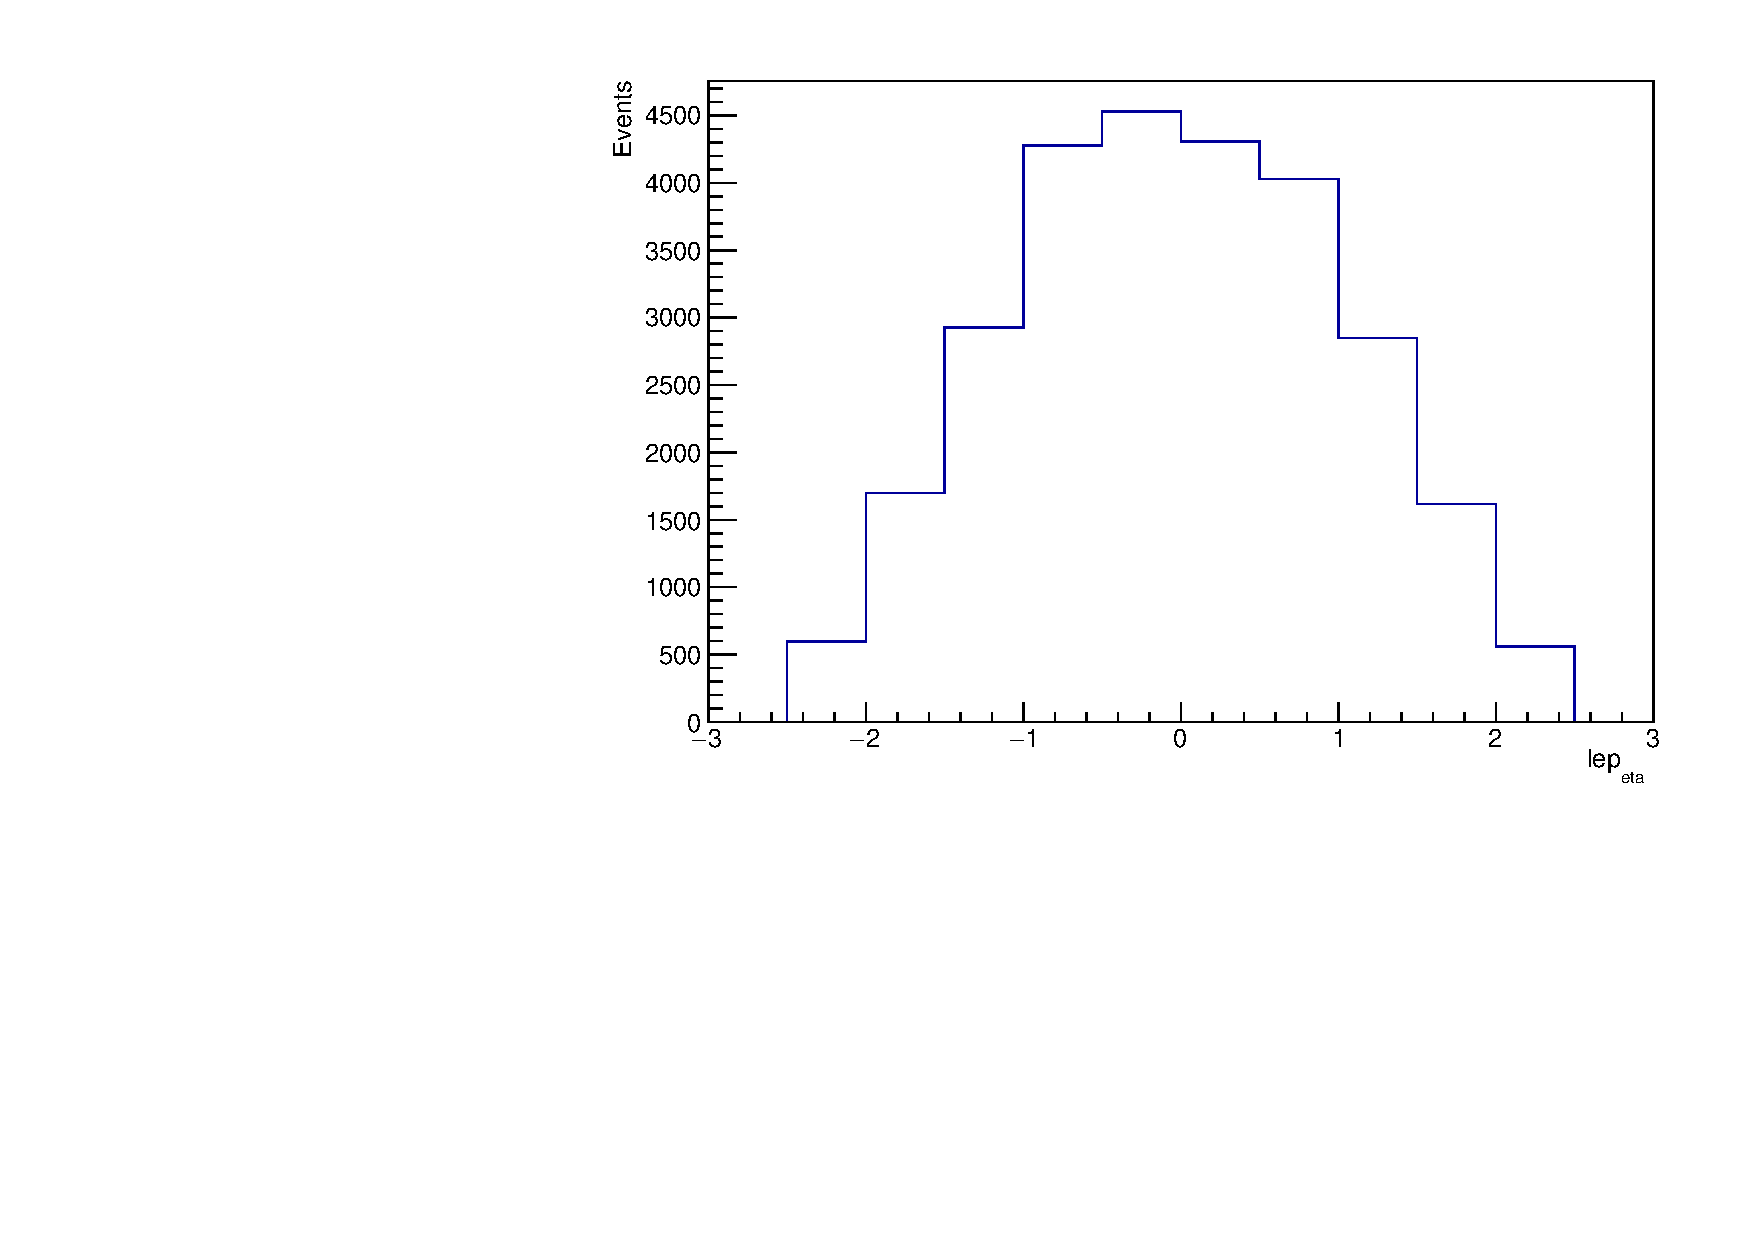
\includegraphics[width=\linewidth]{plots_and_txt/ttbar.mu_selected_/ttbar.mu_selected_lep_eta.pdf}
    \caption{}
    \label{fig:lep_pt2}
  \end{subfigure}%
  \begin{subfigure}{0.5\textwidth}
    \centering
    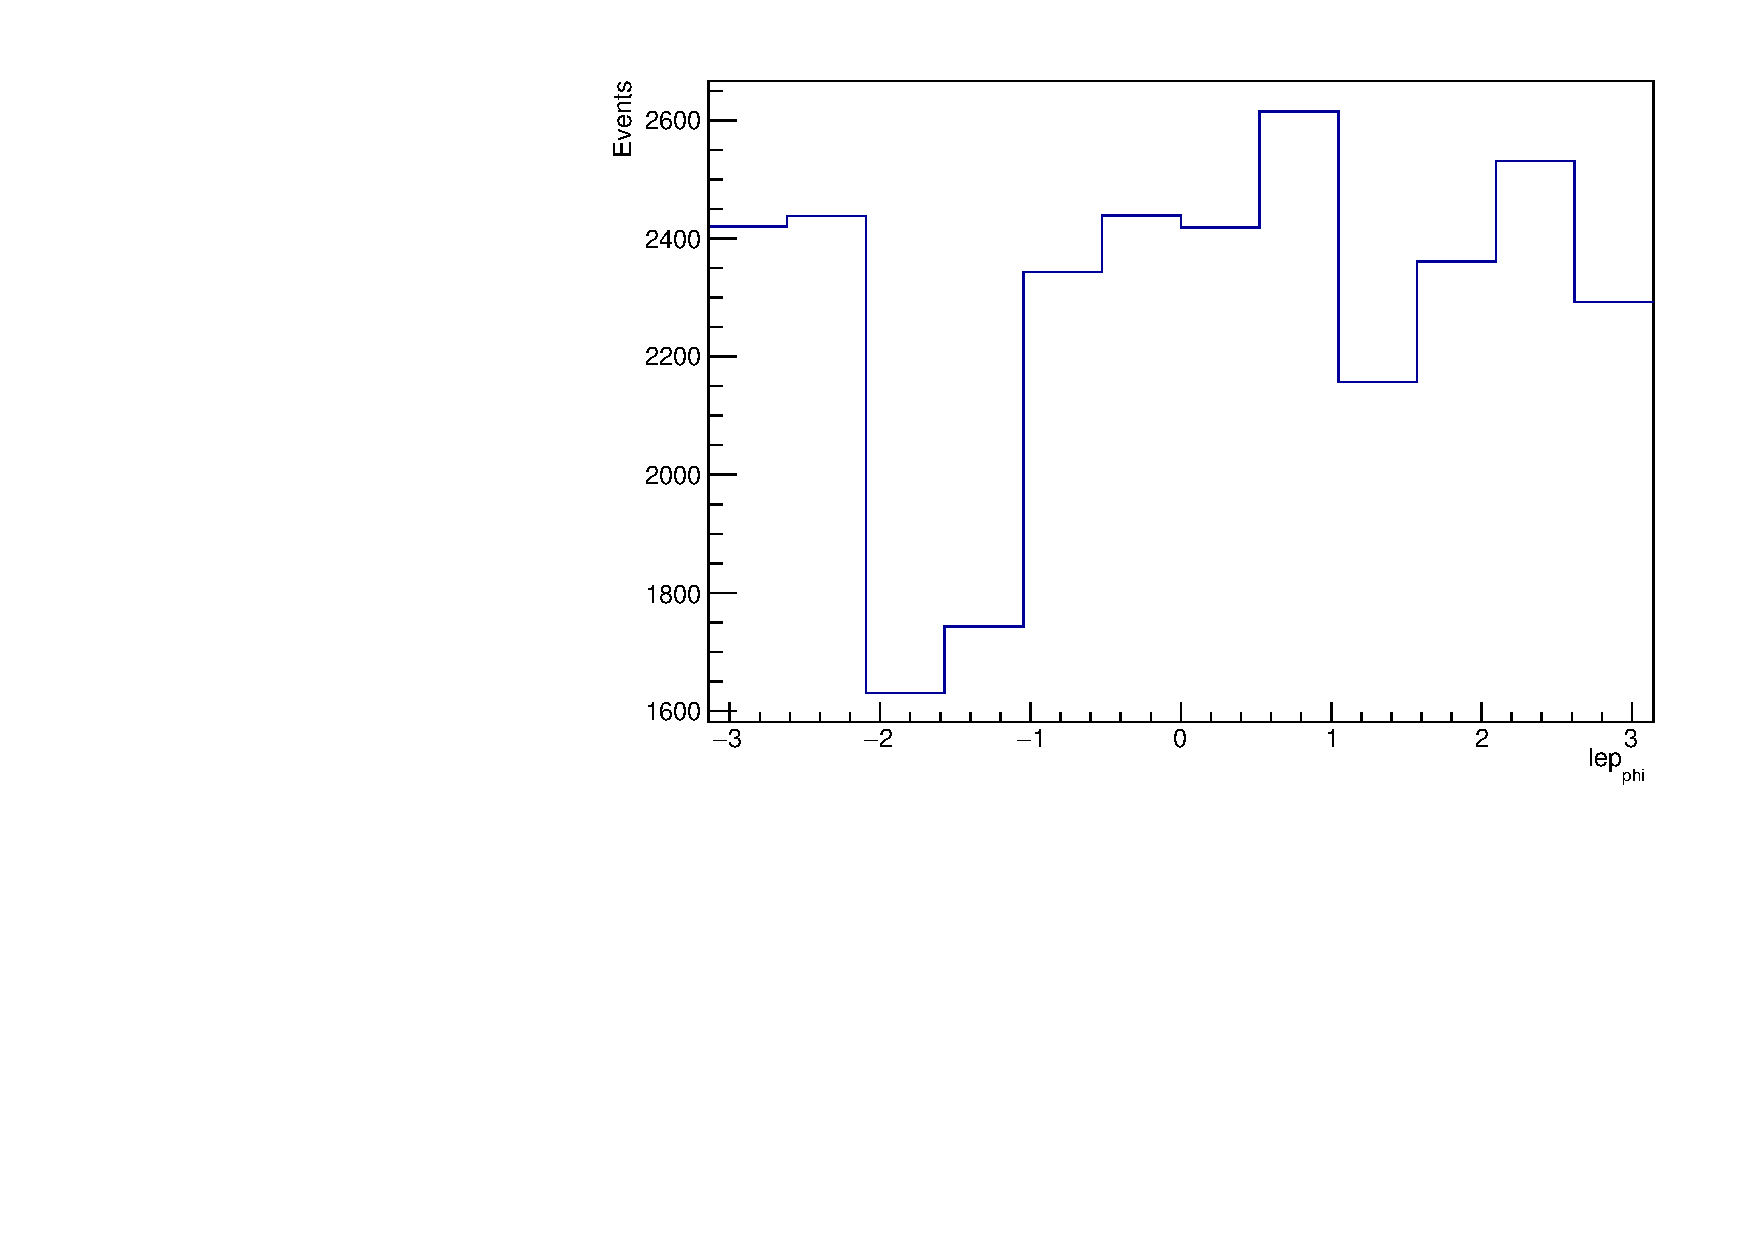
\includegraphics[width=\linewidth]{plots_and_txt/ttbar.mu_selected_/ttbar.mu_selected_lep_phi.pdf}
    \caption{}
    \label{fig:btagged2}
  \end{subfigure}%
  \newline
  \begin{subfigure}{0.5\textwidth}
    \centering
    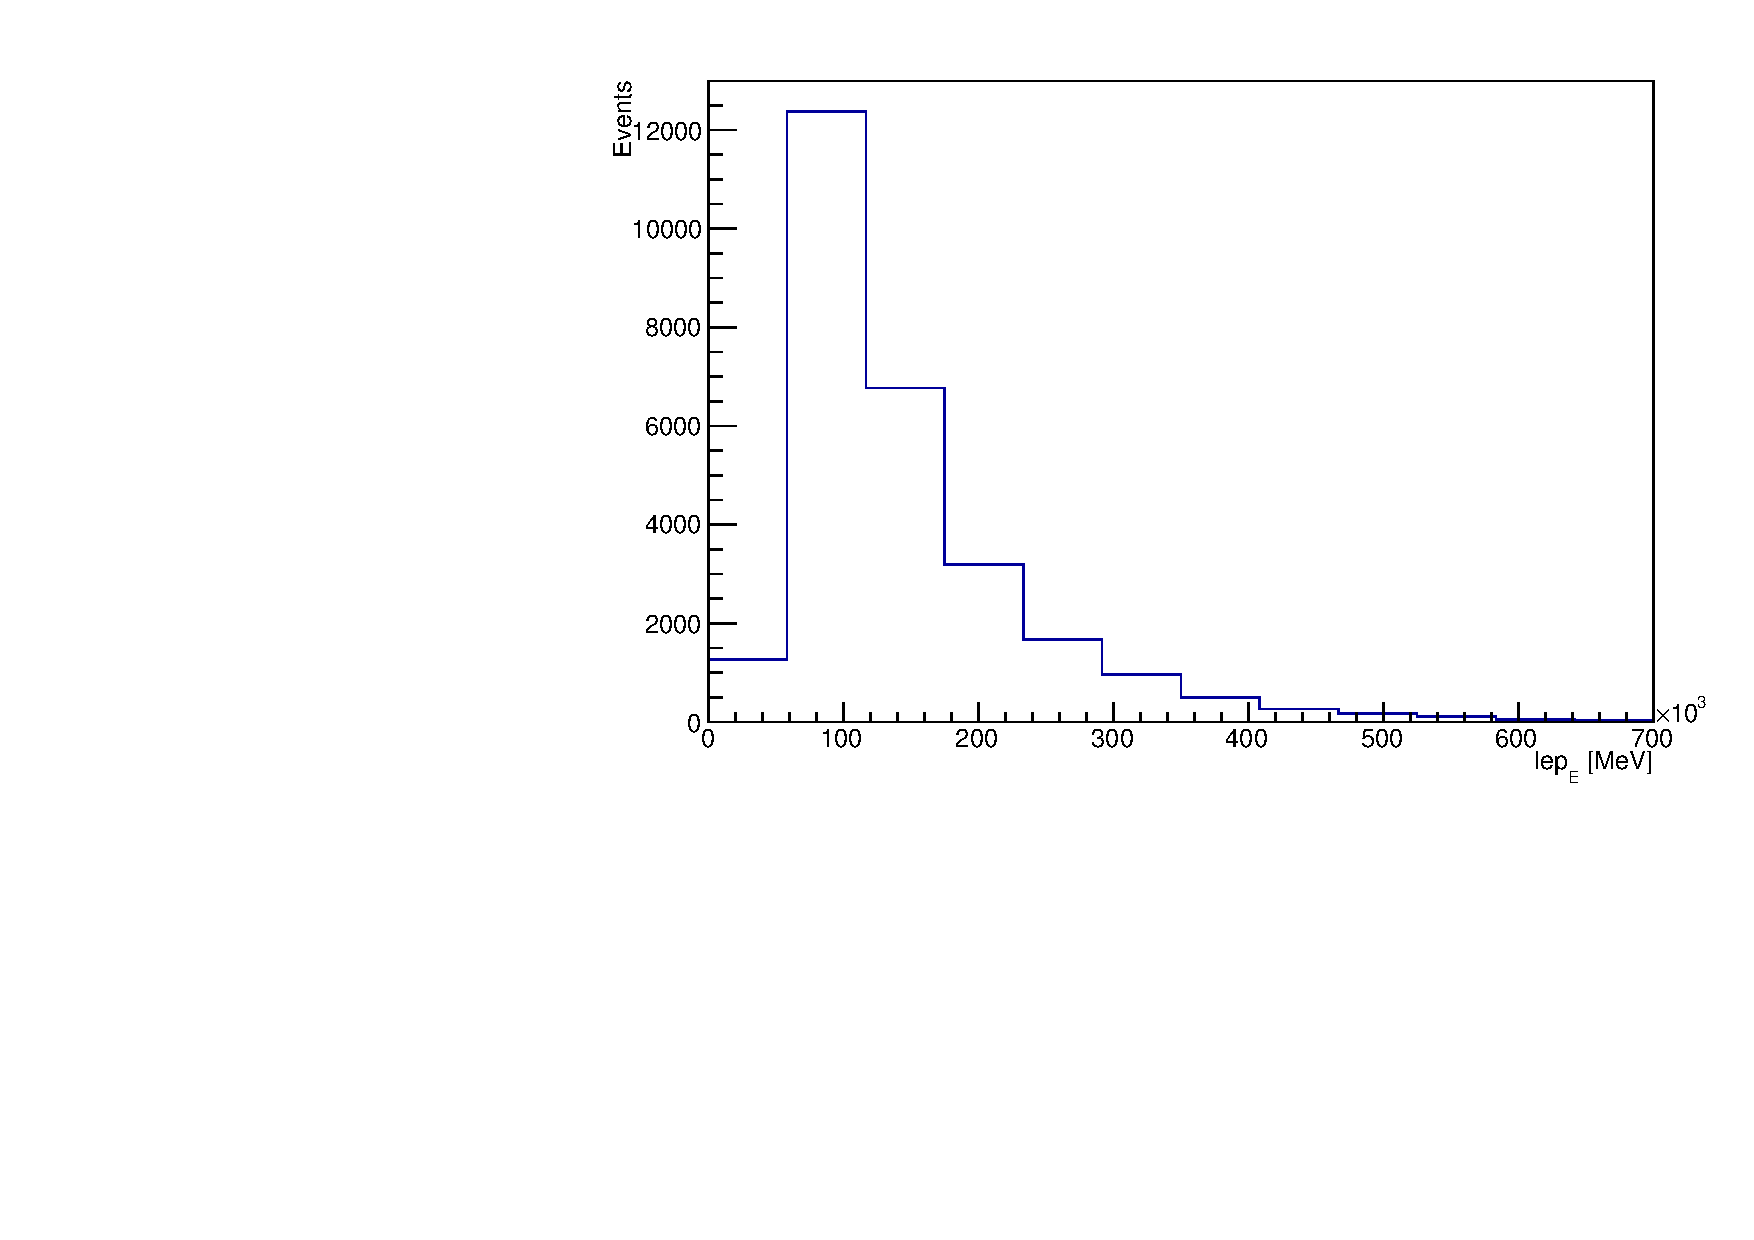
\includegraphics[width=\linewidth]{plots_and_txt/ttbar.mu_selected_/ttbar.mu_selected_lep_E.pdf}
    \caption{}
    \label{fig:jet_pt_good2}
  \end{subfigure}%
  \begin{subfigure}{0.5\textwidth}
    \centering
    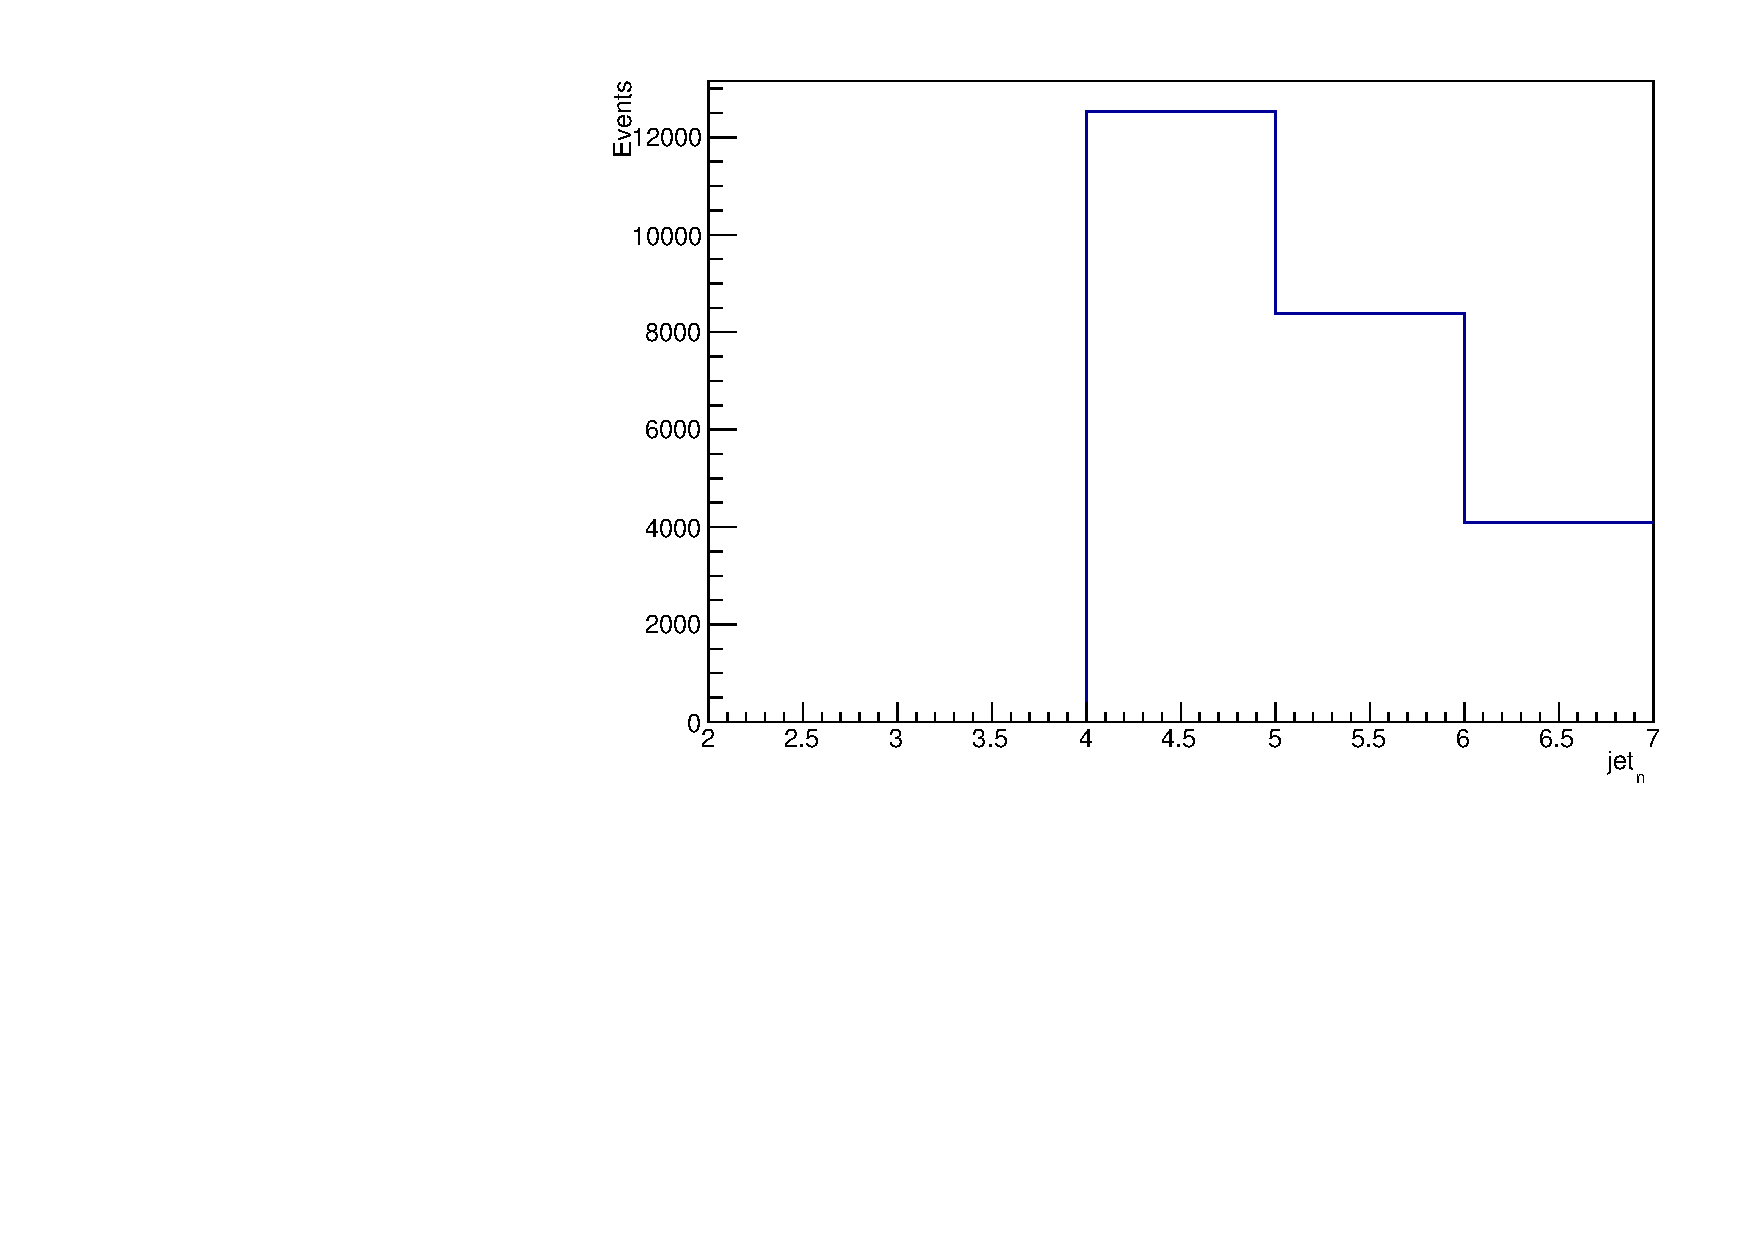
\includegraphics[width=\linewidth]{plots_and_txt/ttbar.mu_selected_/ttbar.mu_selected_jet_n.pdf}
    \caption{}
    \label{fig:met_et2}
  \end{subfigure}%
  \caption{Darstellung verschiedener Verteilungen der Größen der $t\bar{t}$ Monte-Carlo Simulation.
  Zusehen sind die Pseudorapidität der Myonen (\subref{fig:lep_pt2}), der Azimuthalwinkel der Leptonen (\subref{fig:btagged2}), der Energie der Myonen (\subref{fig:jet_pt_good2}) und die Anzahl an nutzbaren Jets (\subref{fig:met_et2}).
  }
  \label{fig:Distributions2}
\end{figure}

\begin{figure}[H]
  \begin{subfigure}{0.5\textwidth}
    \centering
    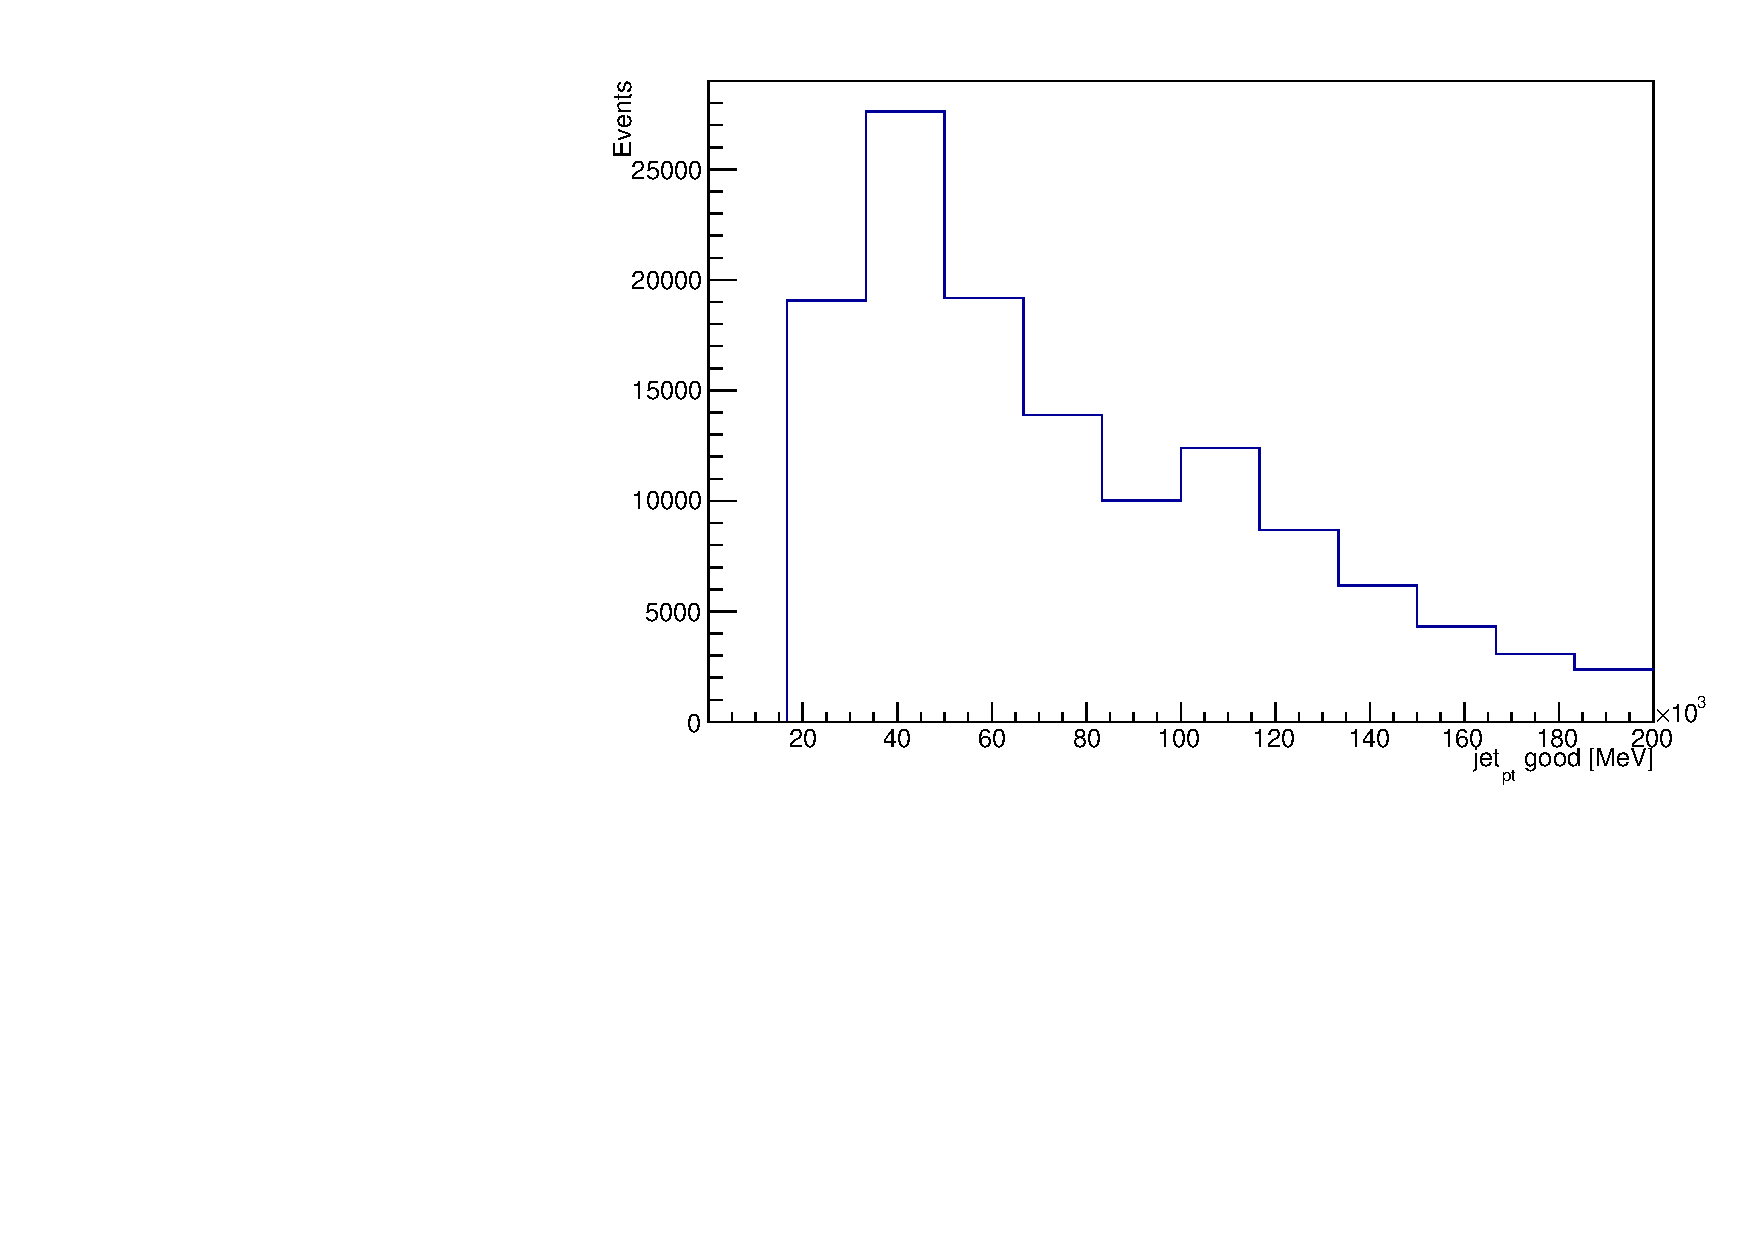
\includegraphics[width=\linewidth]{plots_and_txt/ttbar.mu_selected_/ttbar.mu_selected_jet_pt_good.pdf}
    \caption{}
    \label{fig:lep_pt3}
  \end{subfigure}%
  \begin{subfigure}{0.5\textwidth}
    \centering
    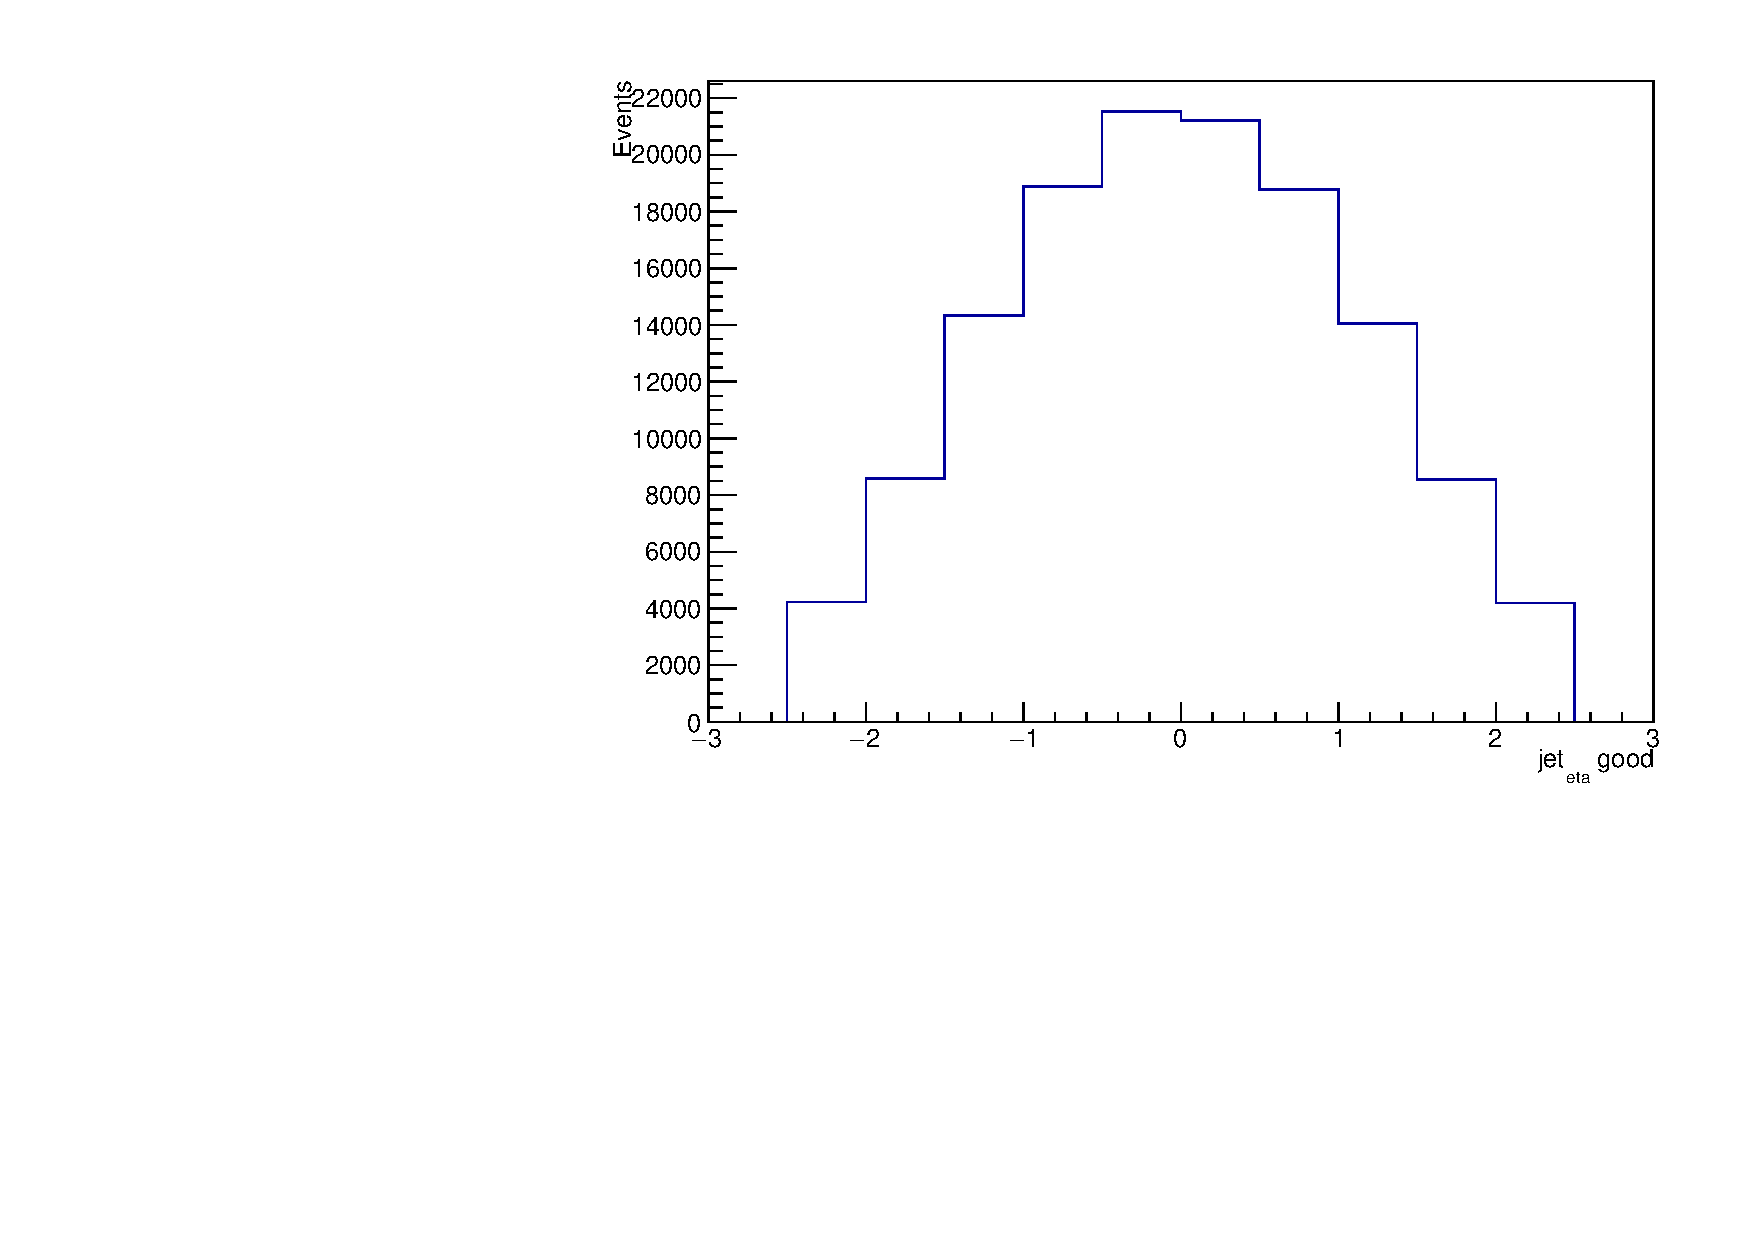
\includegraphics[width=\linewidth]{plots_and_txt/ttbar.mu_selected_/ttbar.mu_selected_jet_eta_good.pdf}
    \caption{}
    \label{fig:btagged3}
  \end{subfigure}%
  \newline
  \begin{subfigure}{0.5\textwidth}
    \centering
    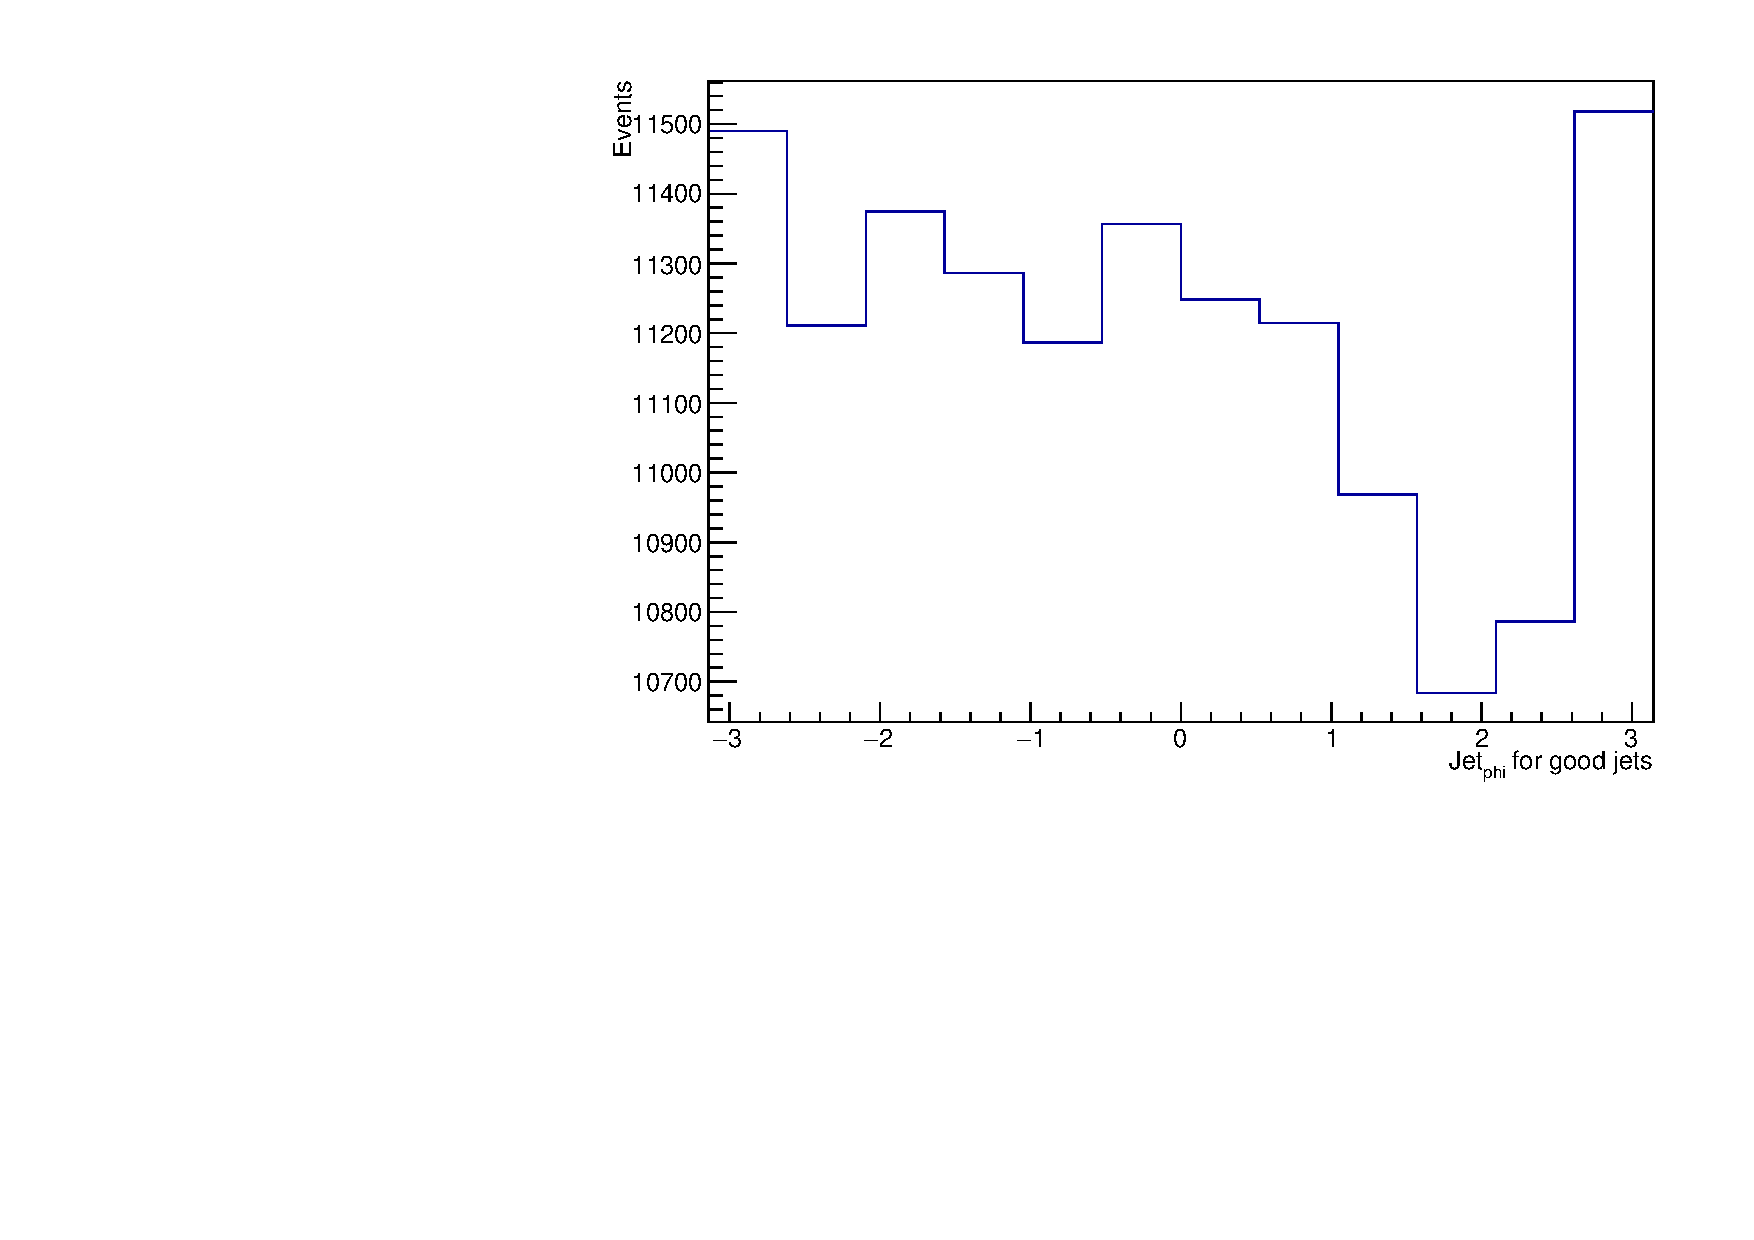
\includegraphics[width=\linewidth]{plots_and_txt/ttbar.mu_selected_/ttbar.mu_selected_jet_phi_good.pdf}
    \caption{}
    \label{fig:jet_pt_good3}
  \end{subfigure}%
  \begin{subfigure}{0.5\textwidth}
    \centering
    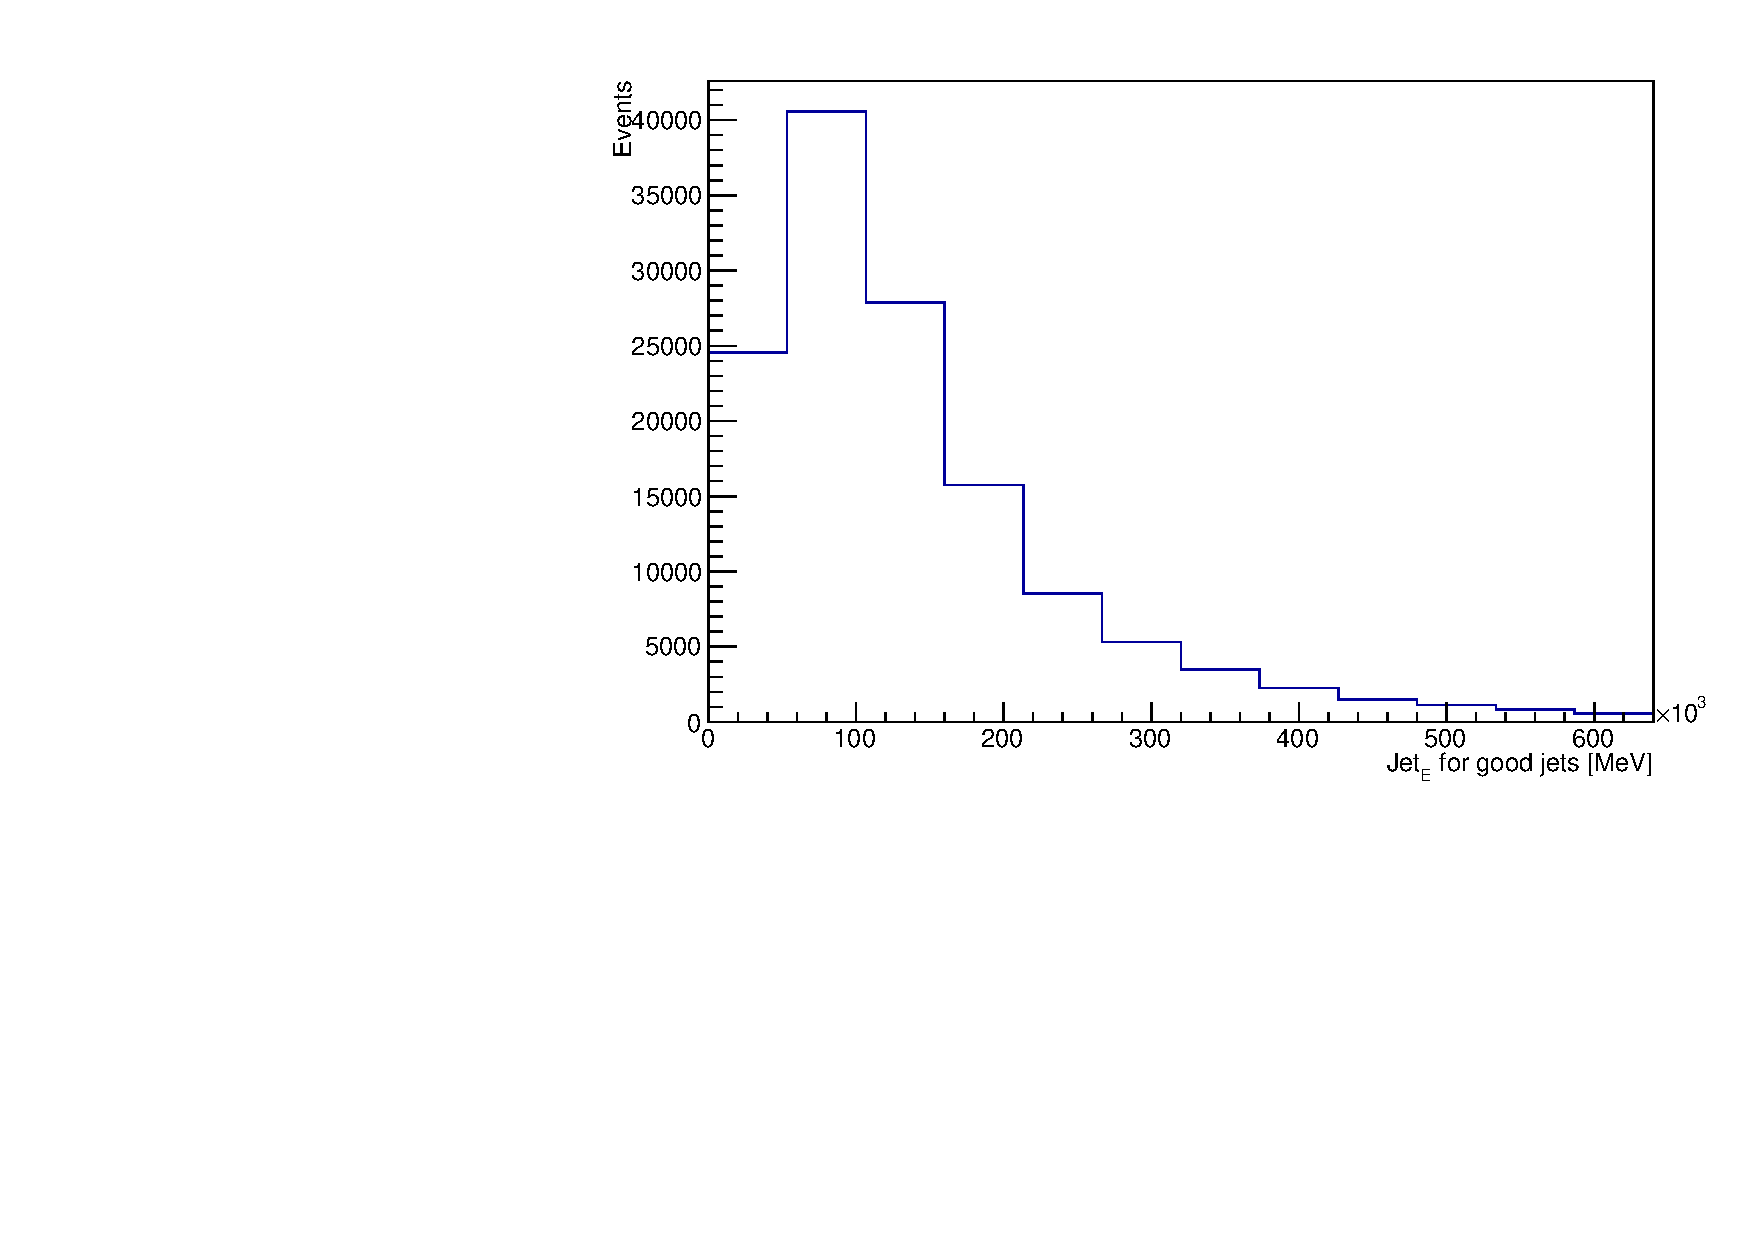
\includegraphics[width=\linewidth]{plots_and_txt/ttbar.mu_selected_/ttbar.mu_selected_jet_E_good.pdf}
    \caption{}
    \label{fig:met_et3}
  \end{subfigure}%
  \caption{Darstellung verschiedener Verteilungen der Größen der $t\bar{t}$ Monte-Carlo Simulation.
  Zusehen sind der transverale Impuls der nutzbaren Jets (\subref{fig:lep_pt3}), die Pseudorapidität der nutzbaren Jets (\subref{fig:btagged3}), der Azimuthalwinkel der nutzbaren Jets (\subref{fig:jet_pt_good3}) und die Energie der nutzbaren Jets (\subref{fig:met_et3}).
  }
  \label{fig:Distributions3}
\end{figure}

\begin{figure}[H]
  \begin{subfigure}{0.5\textwidth}
    \centering
    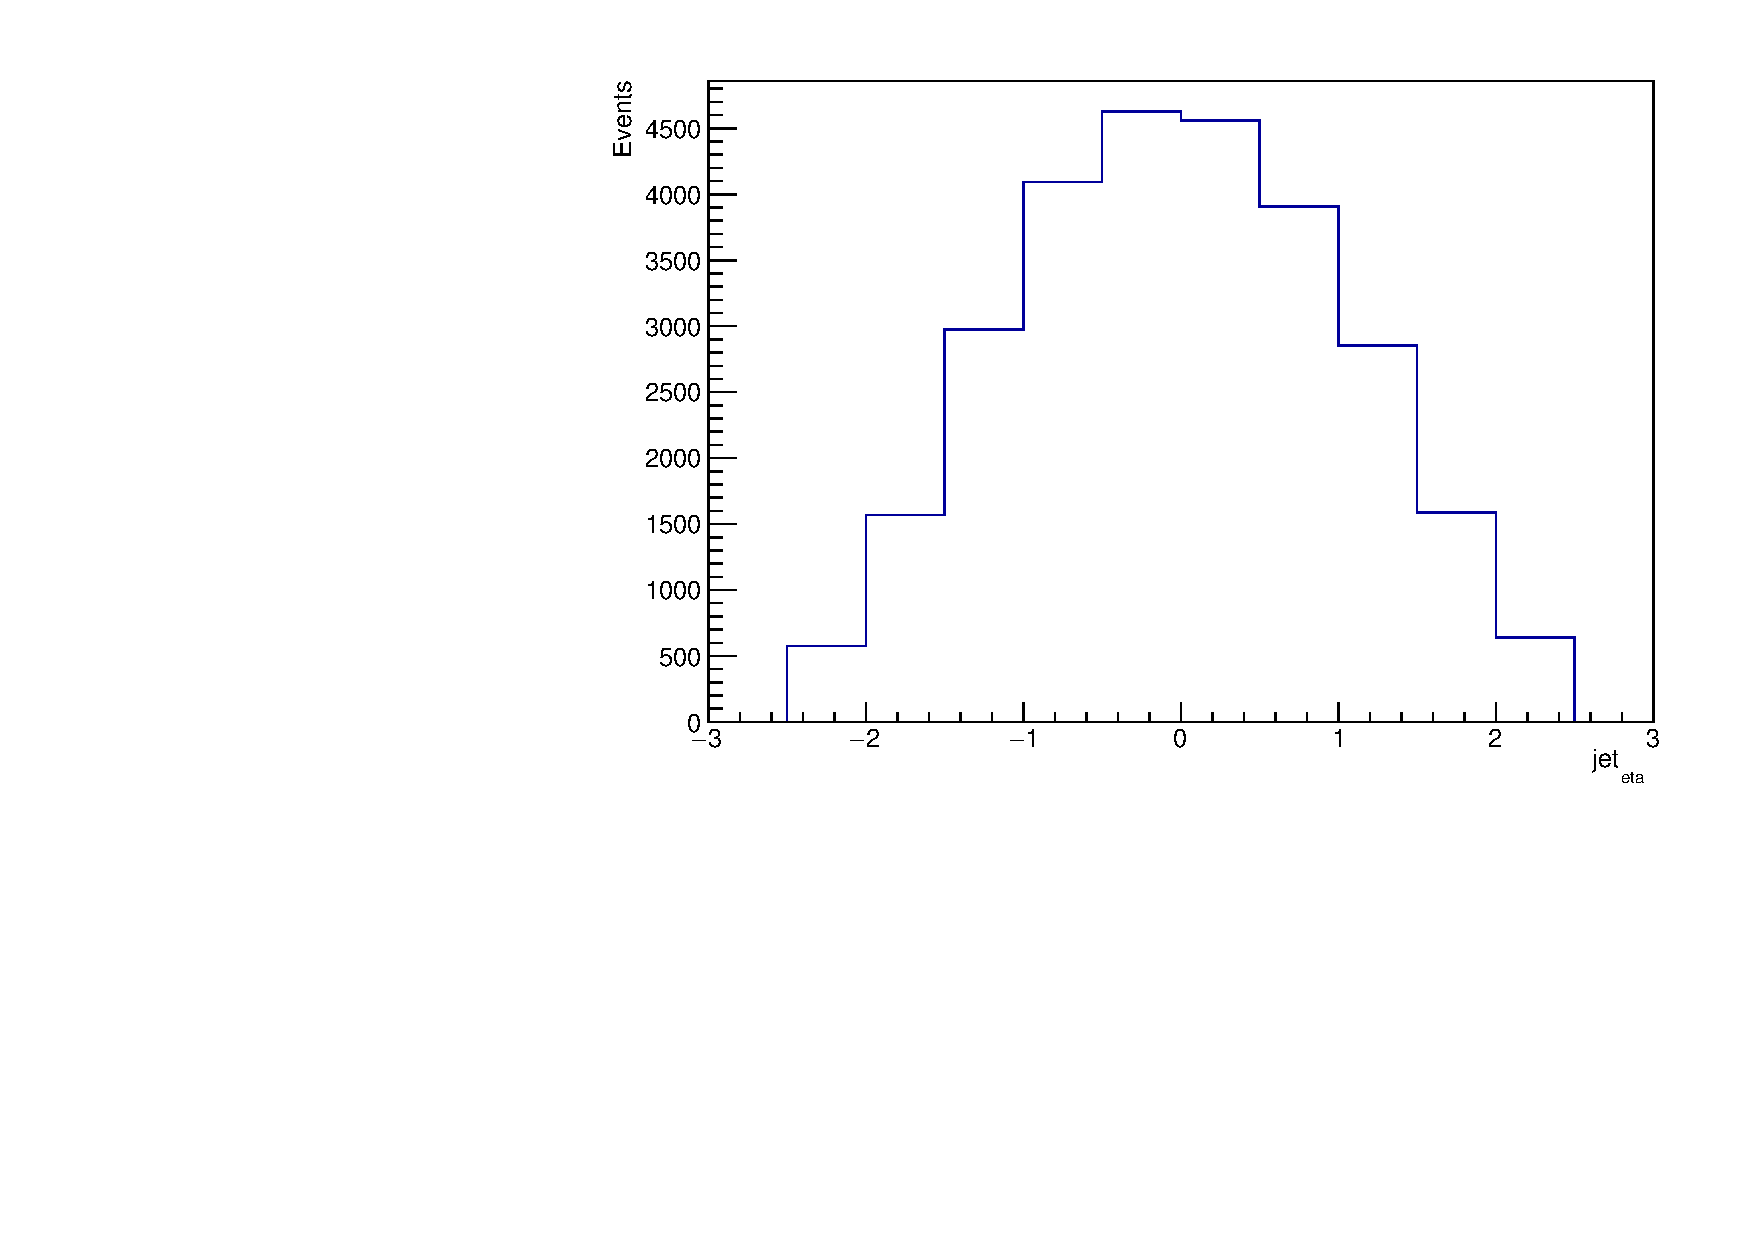
\includegraphics[width=\linewidth]{plots_and_txt/ttbar.mu_selected_/ttbar.mu_selected_jet_eta.pdf}
    \caption{}
    \label{fig:lep_pt4}
  \end{subfigure}%
  \begin{subfigure}{0.5\textwidth}
    \centering
    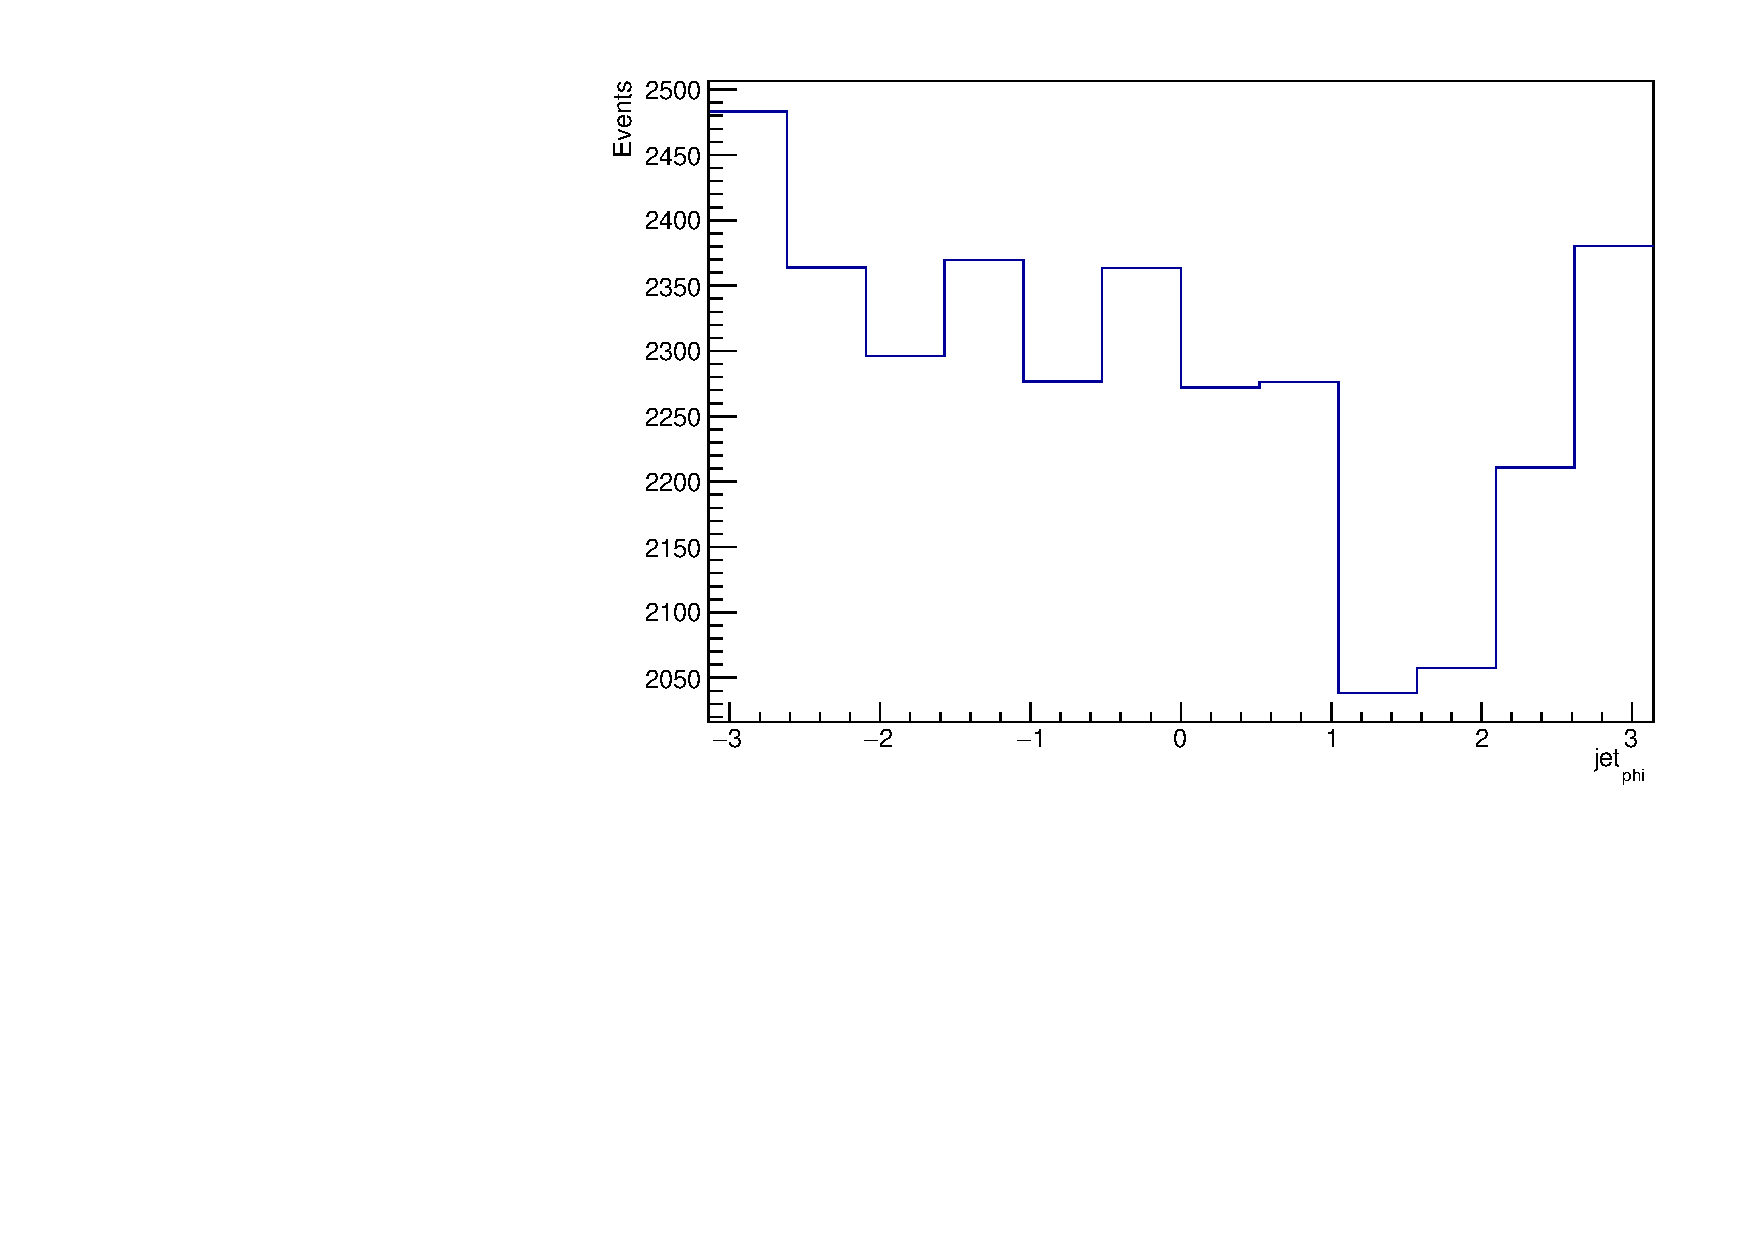
\includegraphics[width=\linewidth]{plots_and_txt/ttbar.mu_selected_/ttbar.mu_selected_jet_phi.pdf}
    \caption{}
    \label{fig:btagged4}
  \end{subfigure}%
  \newline
  \begin{subfigure}{0.5\textwidth}
    \centering
    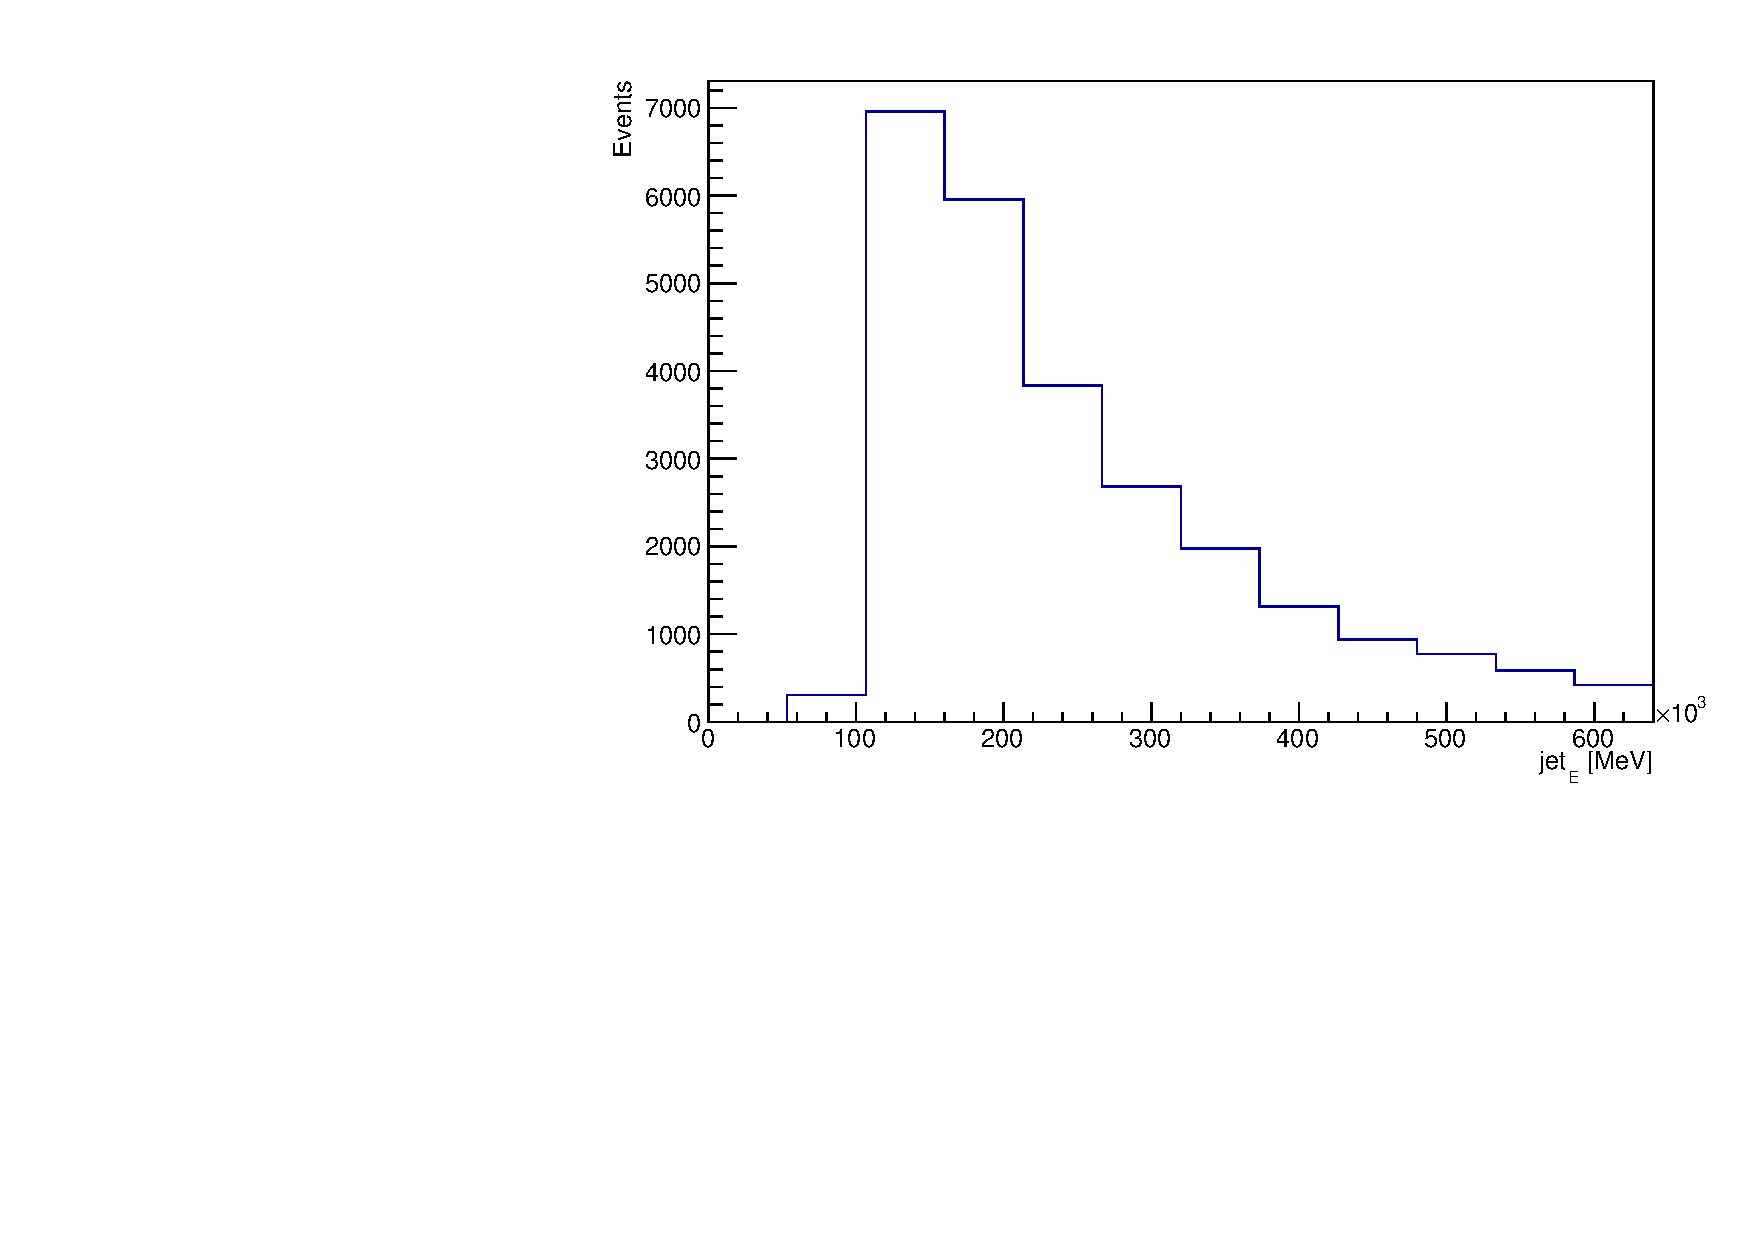
\includegraphics[width=\linewidth]{plots_and_txt/ttbar.mu_selected_/ttbar.mu_selected_jet_E.pdf}
    \caption{}
    \label{fig:jet_pt_good4}
  \end{subfigure}%
  \caption{Darstellung verschiedener Verteilungen der Größen der $t\bar{t}$ Monte-Carlo Simulation.
  Zusehen sind die Pseudorapidität des Jets mit dem höchsten $p_T$ (\subref{fig:lep_pt4}),  der Azimuthalwinkel des Jets mit dem höchsten $p_T$ (\subref{fig:btagged4}) und die Energie des Jets mit dem höchsten $p_T$ (\subref{fig:jet_pt_good4}).
  }
  \label{fig:Distributions4}
\end{figure}

\begin{figure}[H]
  \begin{subfigure}{0.5\textwidth}
    \centering
    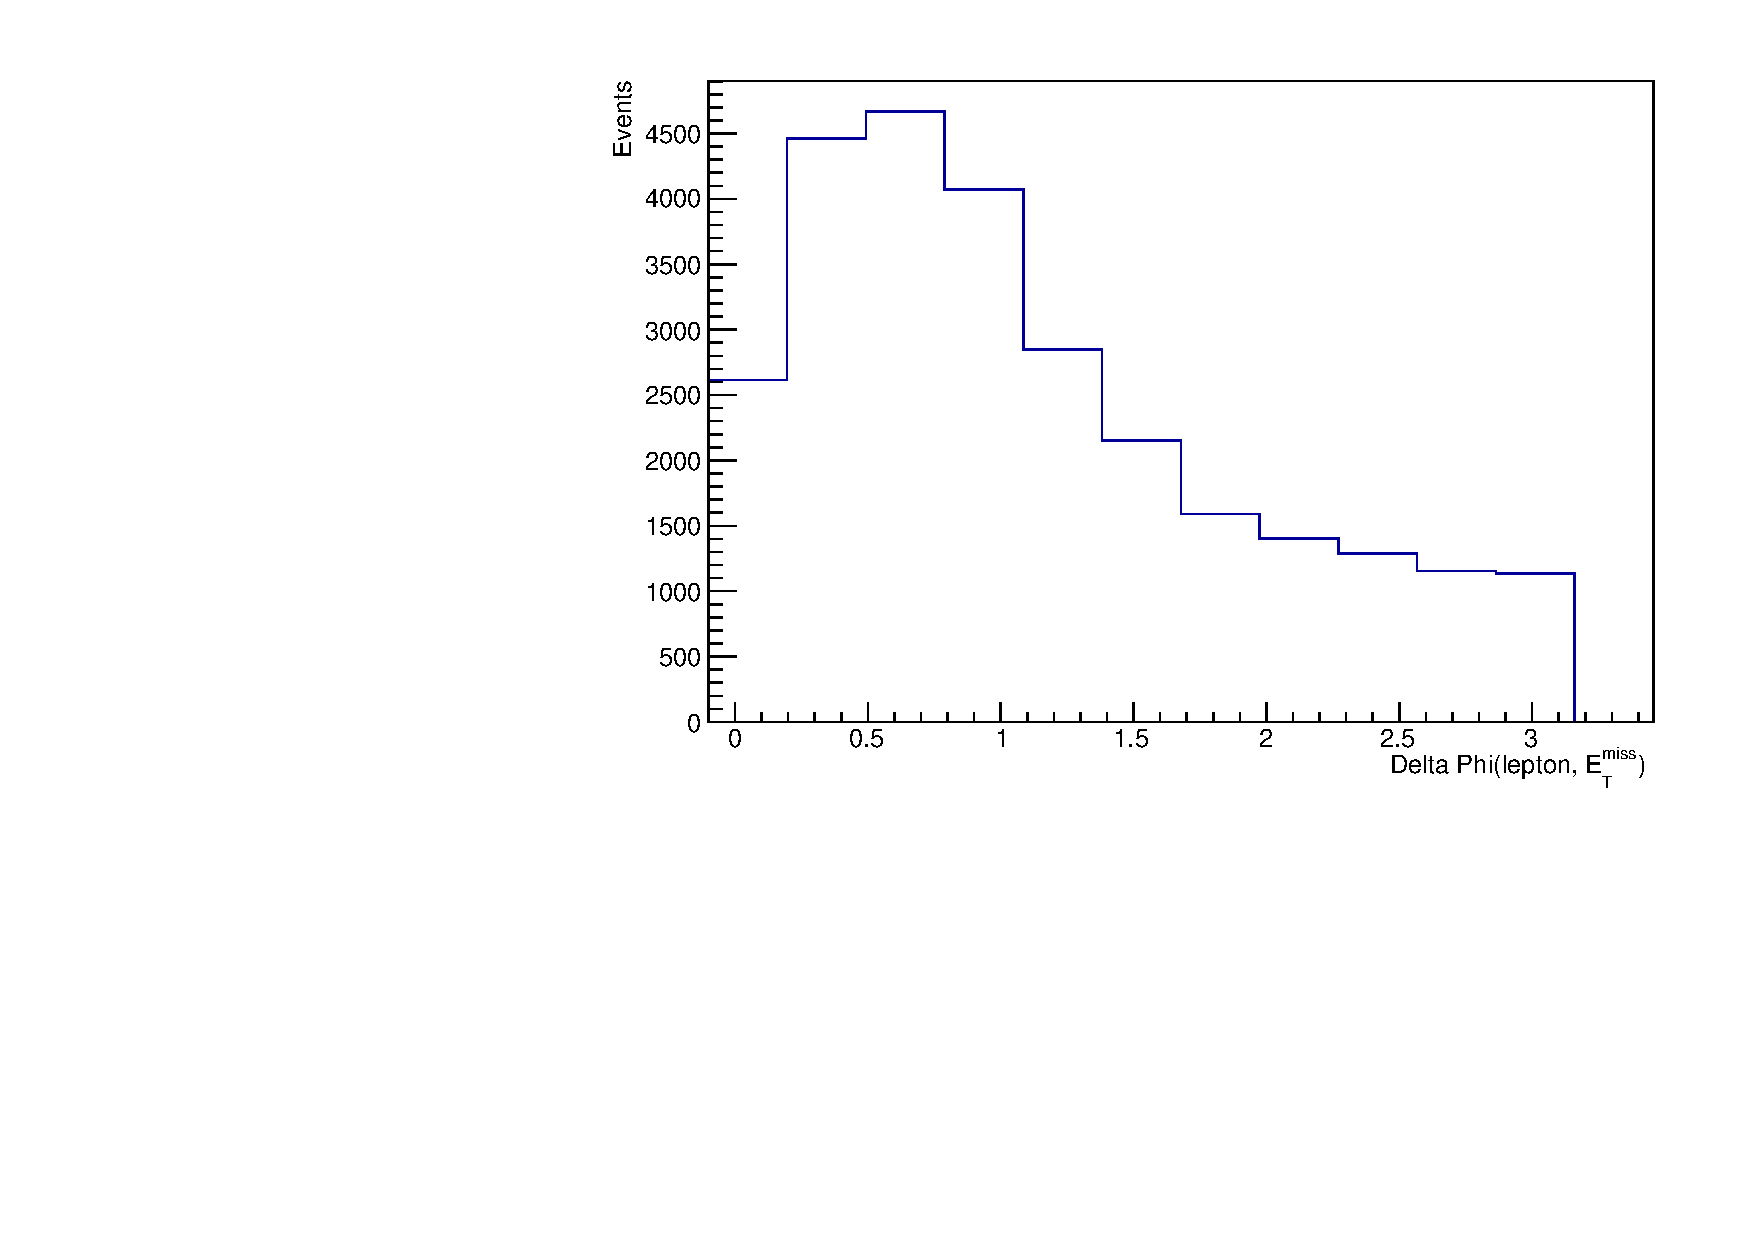
\includegraphics[width=\linewidth]{plots_and_txt/ttbar.mu_selected_/ttbar.mu_selected_DeltaPhi.pdf}
    \caption{}
    \label{fig:ttbar_sys1}
  \end{subfigure}%
  \begin{subfigure}{0.5\textwidth}
    \centering
    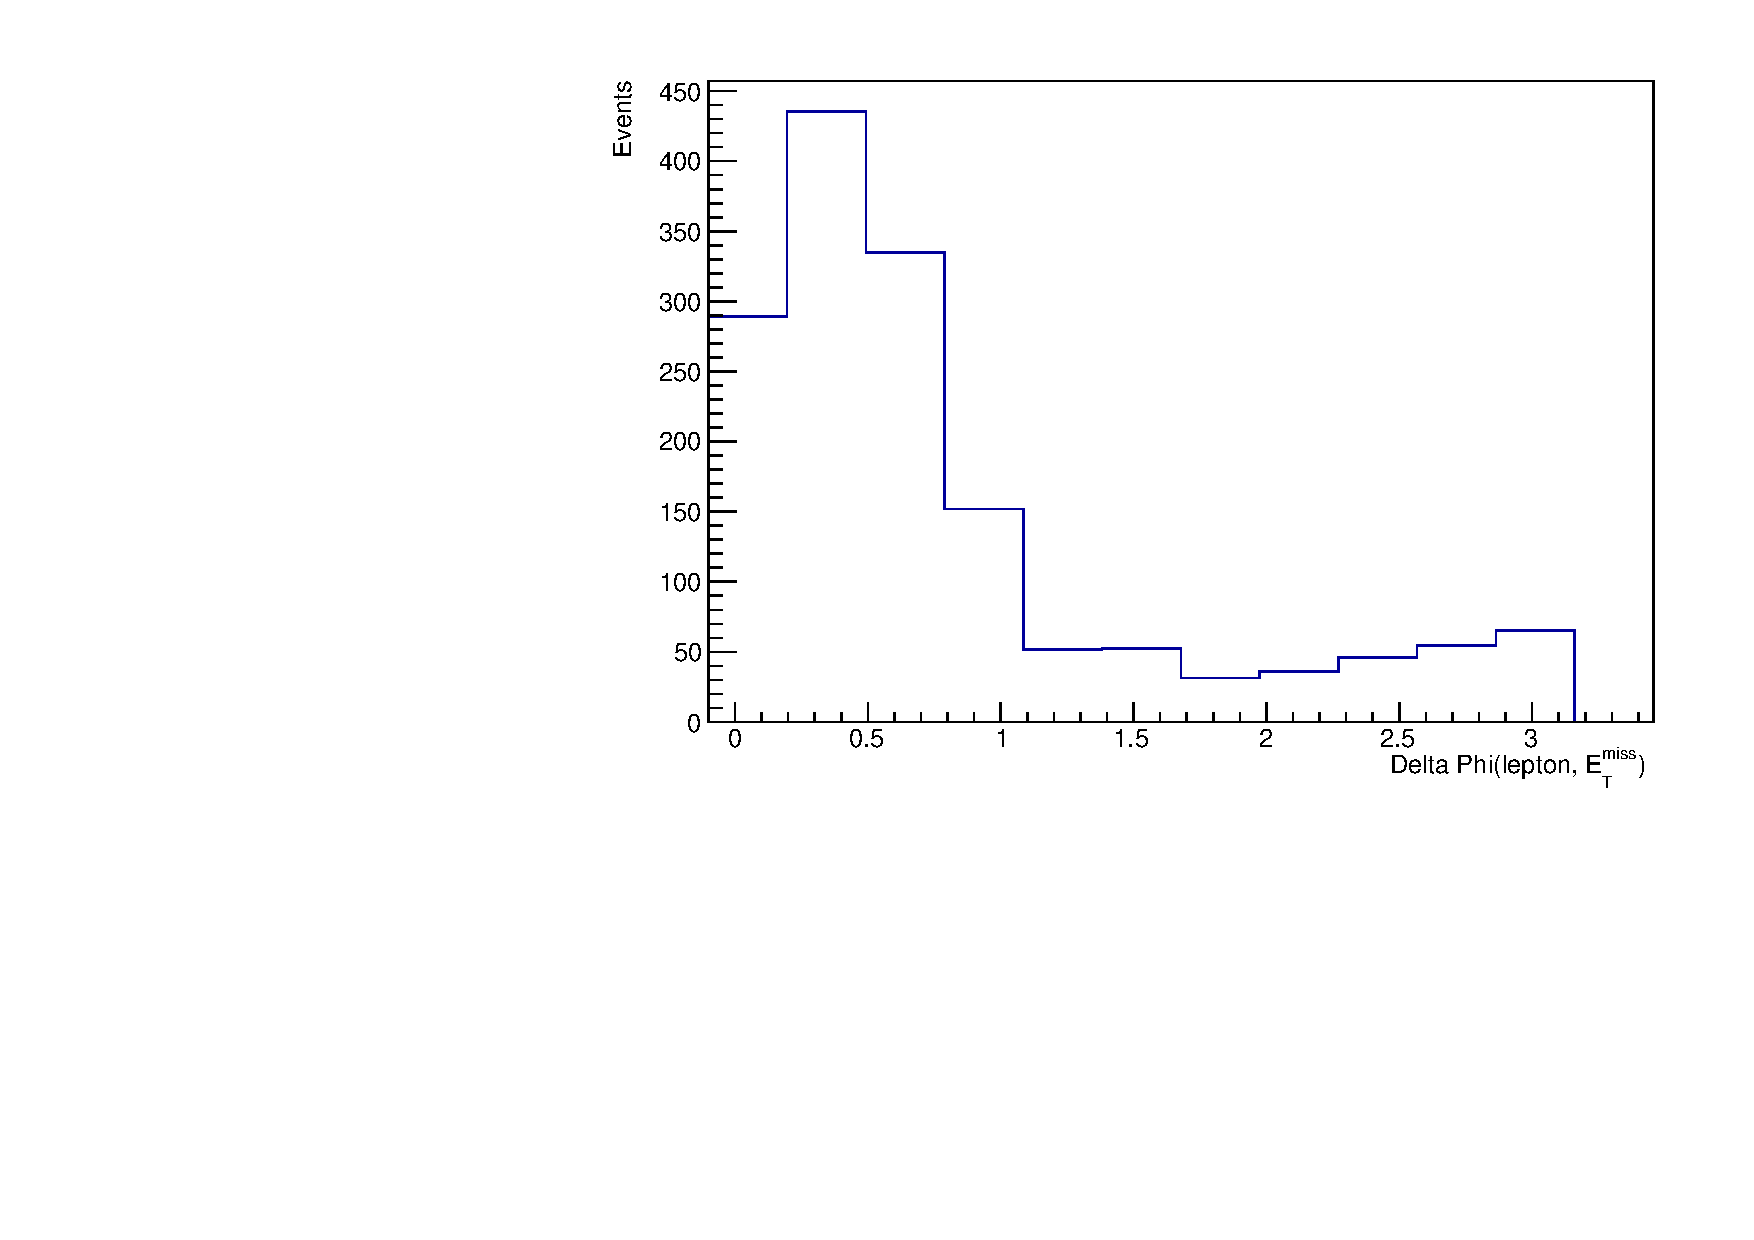
\includegraphics[width=\linewidth]{plots_and_txt/zprime1000.mu_selected_/zprime1000.mu_selected_DeltaPhi.pdf}
    \caption{}
    \label{fig:zprime_sys1}
  \end{subfigure}%
  \caption{Vergleich der Verteilung der Differenz zwischen dem Azimuthalwinkel der fehlenden Transversalenergie und der Leptonflugrichtung.
  Dies ist für die $t\bar{t}$-Untergrundsimulation \subref{fig:ttbar_sys} und der Signalsimulation des $Z^\prime(1000)$ \subref{fig:zprime_sys} dargestellt.
  }
  \label{fig:Comparison1}
\end{figure}

\begin{figure}[H]
  \begin{subfigure}{0.5\textwidth}
    \centering
    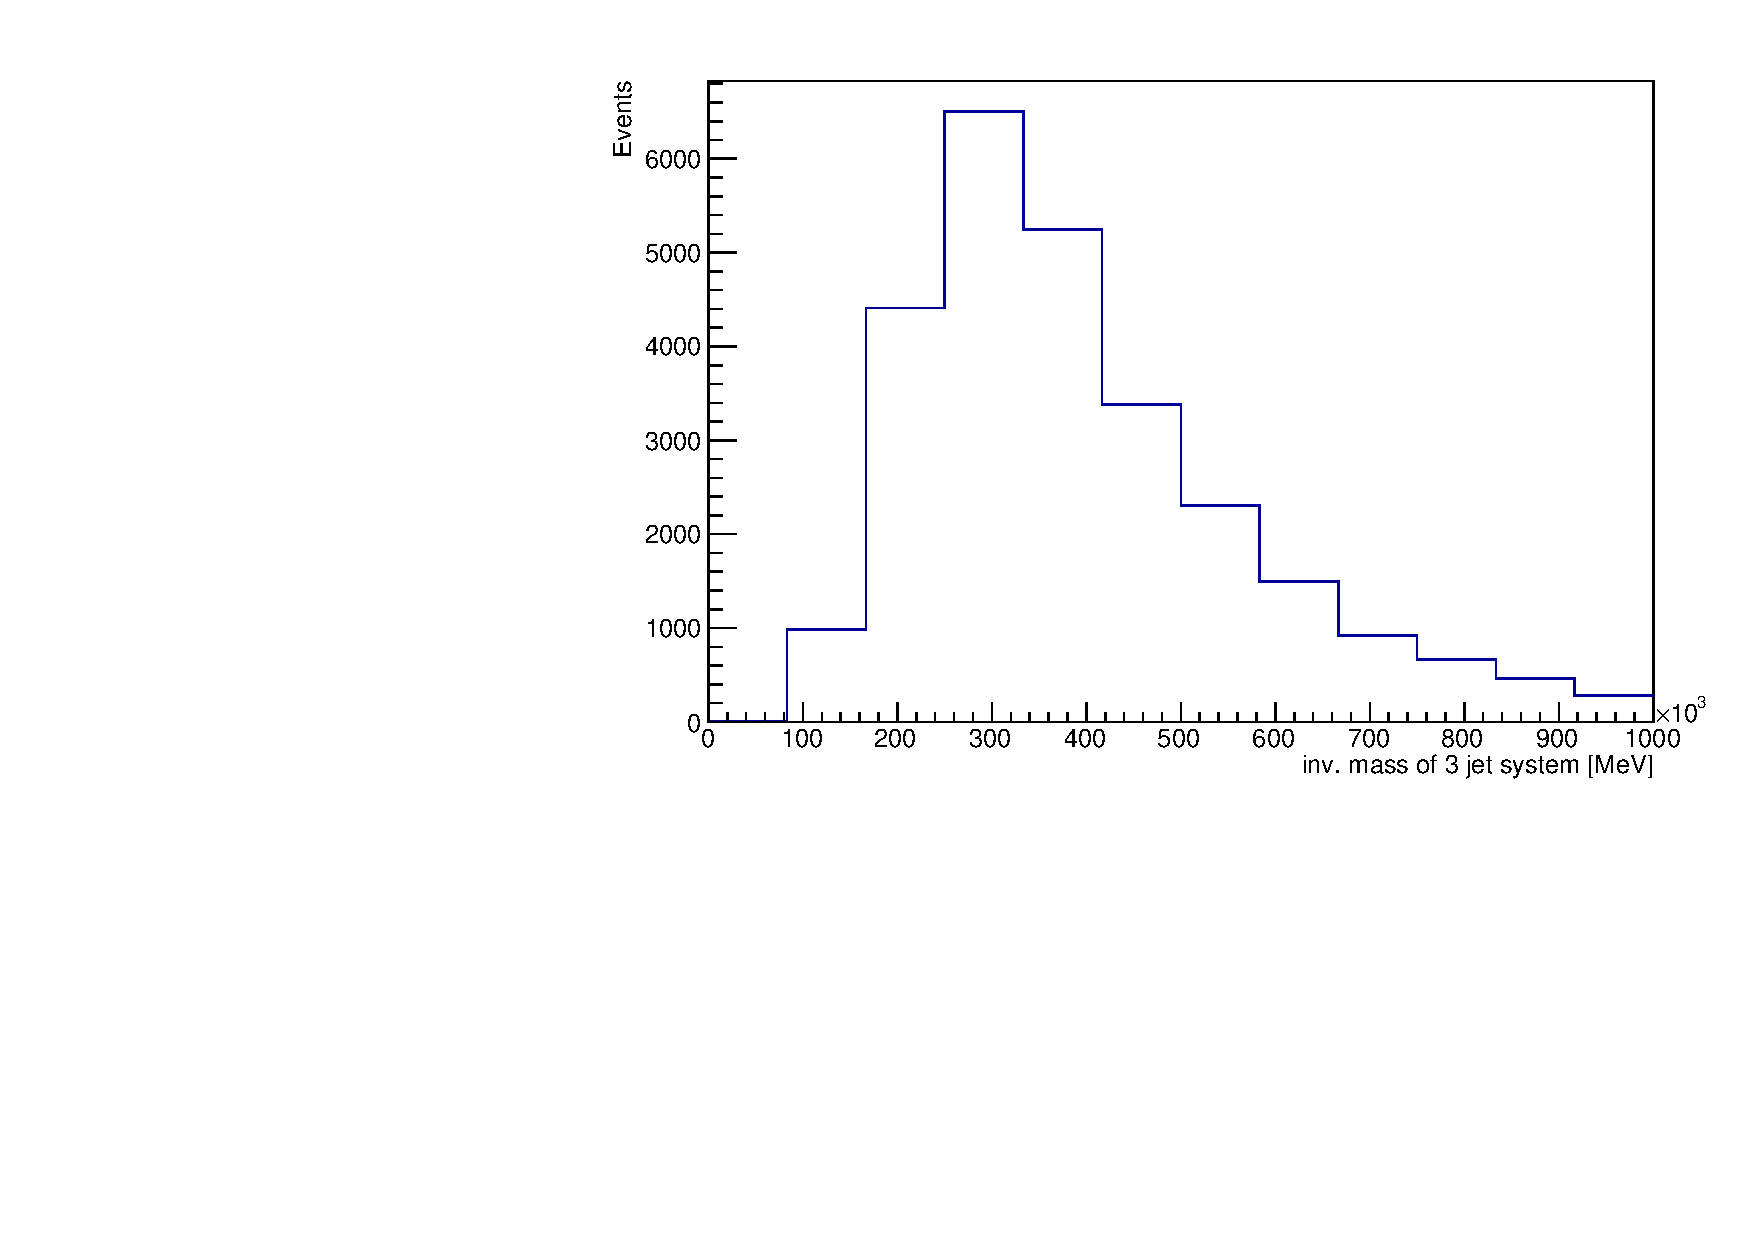
\includegraphics[width=\linewidth]{plots_and_txt/ttbar.mu_selected_/ttbar.mu_selected_InvJetMass.pdf}
    \caption{}
    \label{fig:ttbar_sys2}
  \end{subfigure}%
  \begin{subfigure}{0.5\textwidth}
    \centering
    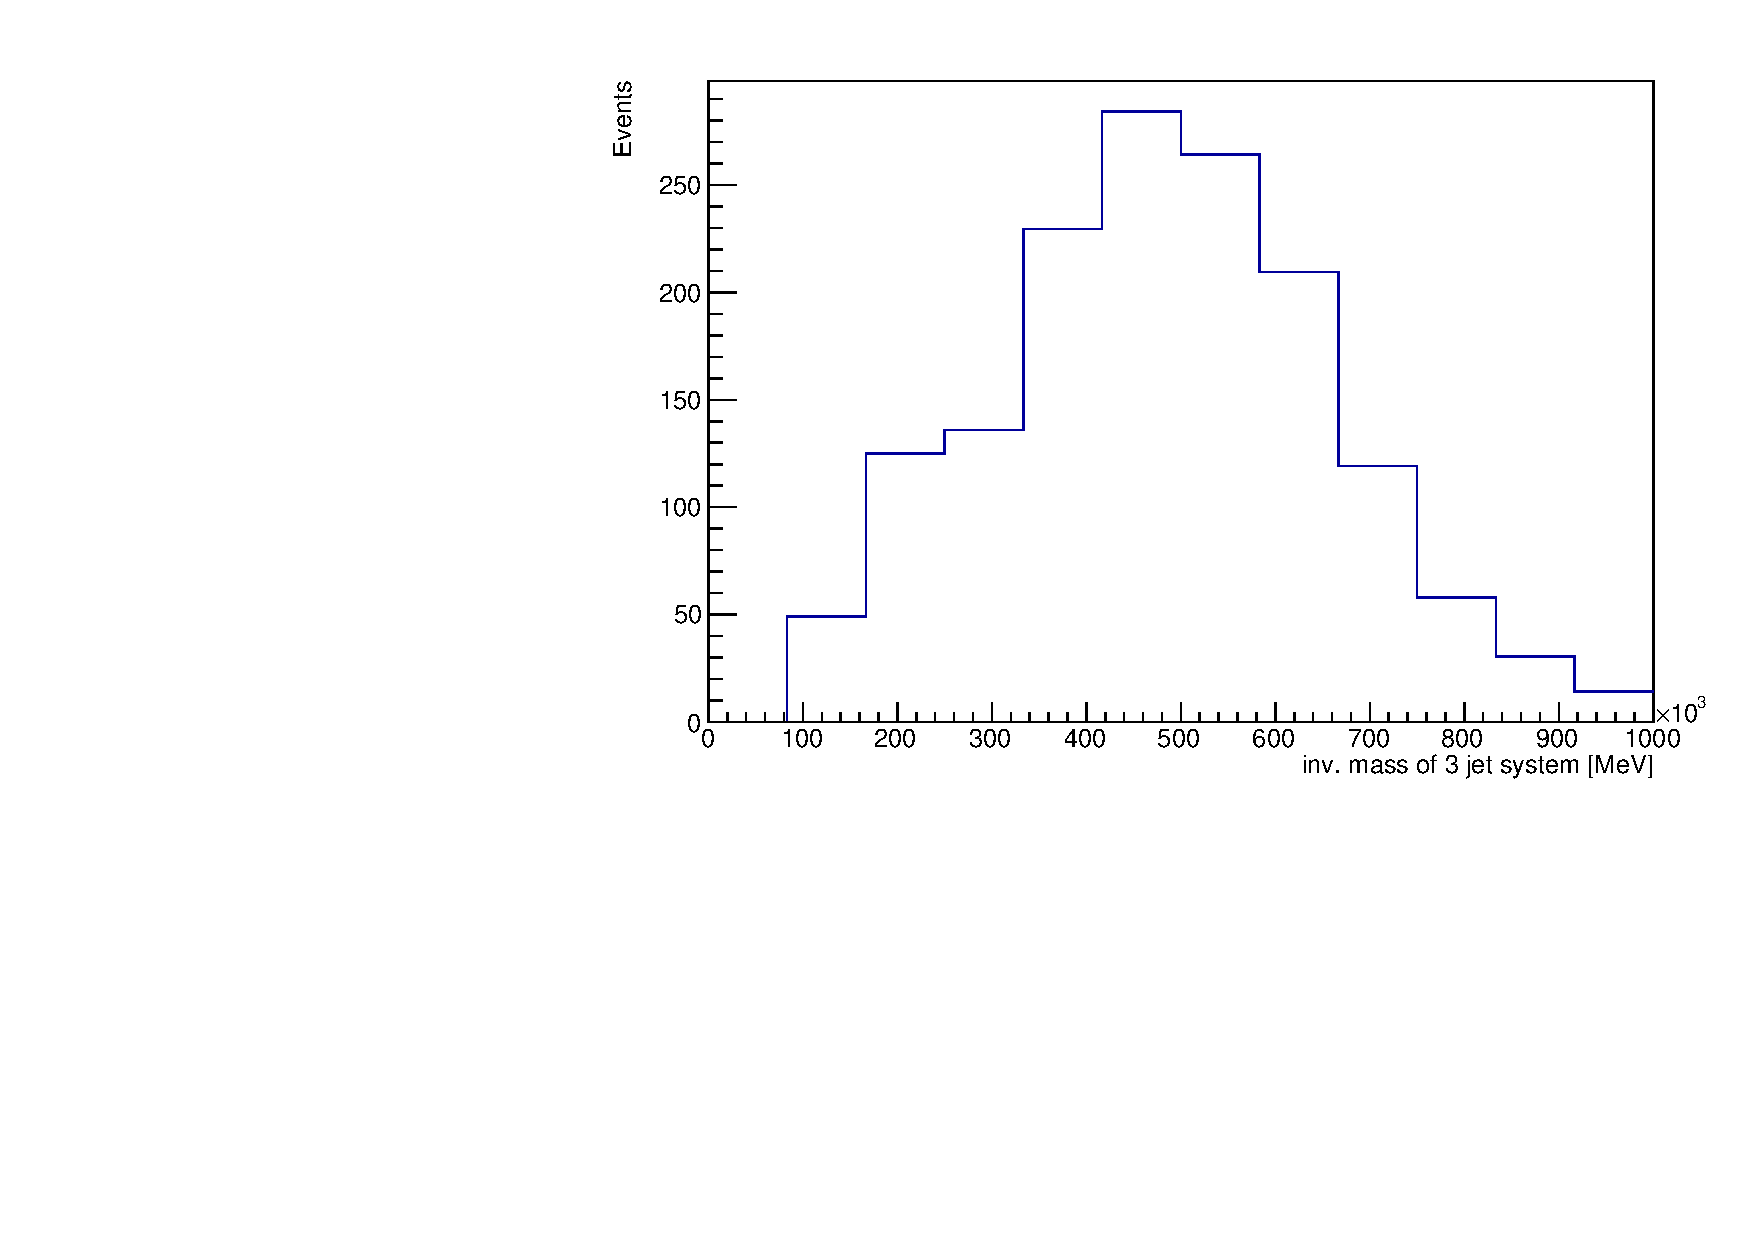
\includegraphics[width=\linewidth]{plots_and_txt/zprime1000.mu_selected_/zprime1000.mu_selected_InvJetMass.pdf}
    \caption{}
    \label{fig:zprime_sys2}
  \end{subfigure}%
  \caption{Vergleich der Verteilung der invarianten Masse des Systems, die durch die drei Jets mit dem größten $p_T$ gebildet wird.
  Dies ist für die $t\bar{t}$-Untergrundsimulation \subref{fig:ttbar_sys2} und der Signalsimulation des $Z^\prime(1000)$ \subref{fig:zprime_sys2} dargestellt.
  }
  \label{fig:Comparison2}
\end{figure}

\begin{figure}[H]
  \begin{subfigure}{0.5\textwidth}
    \centering
    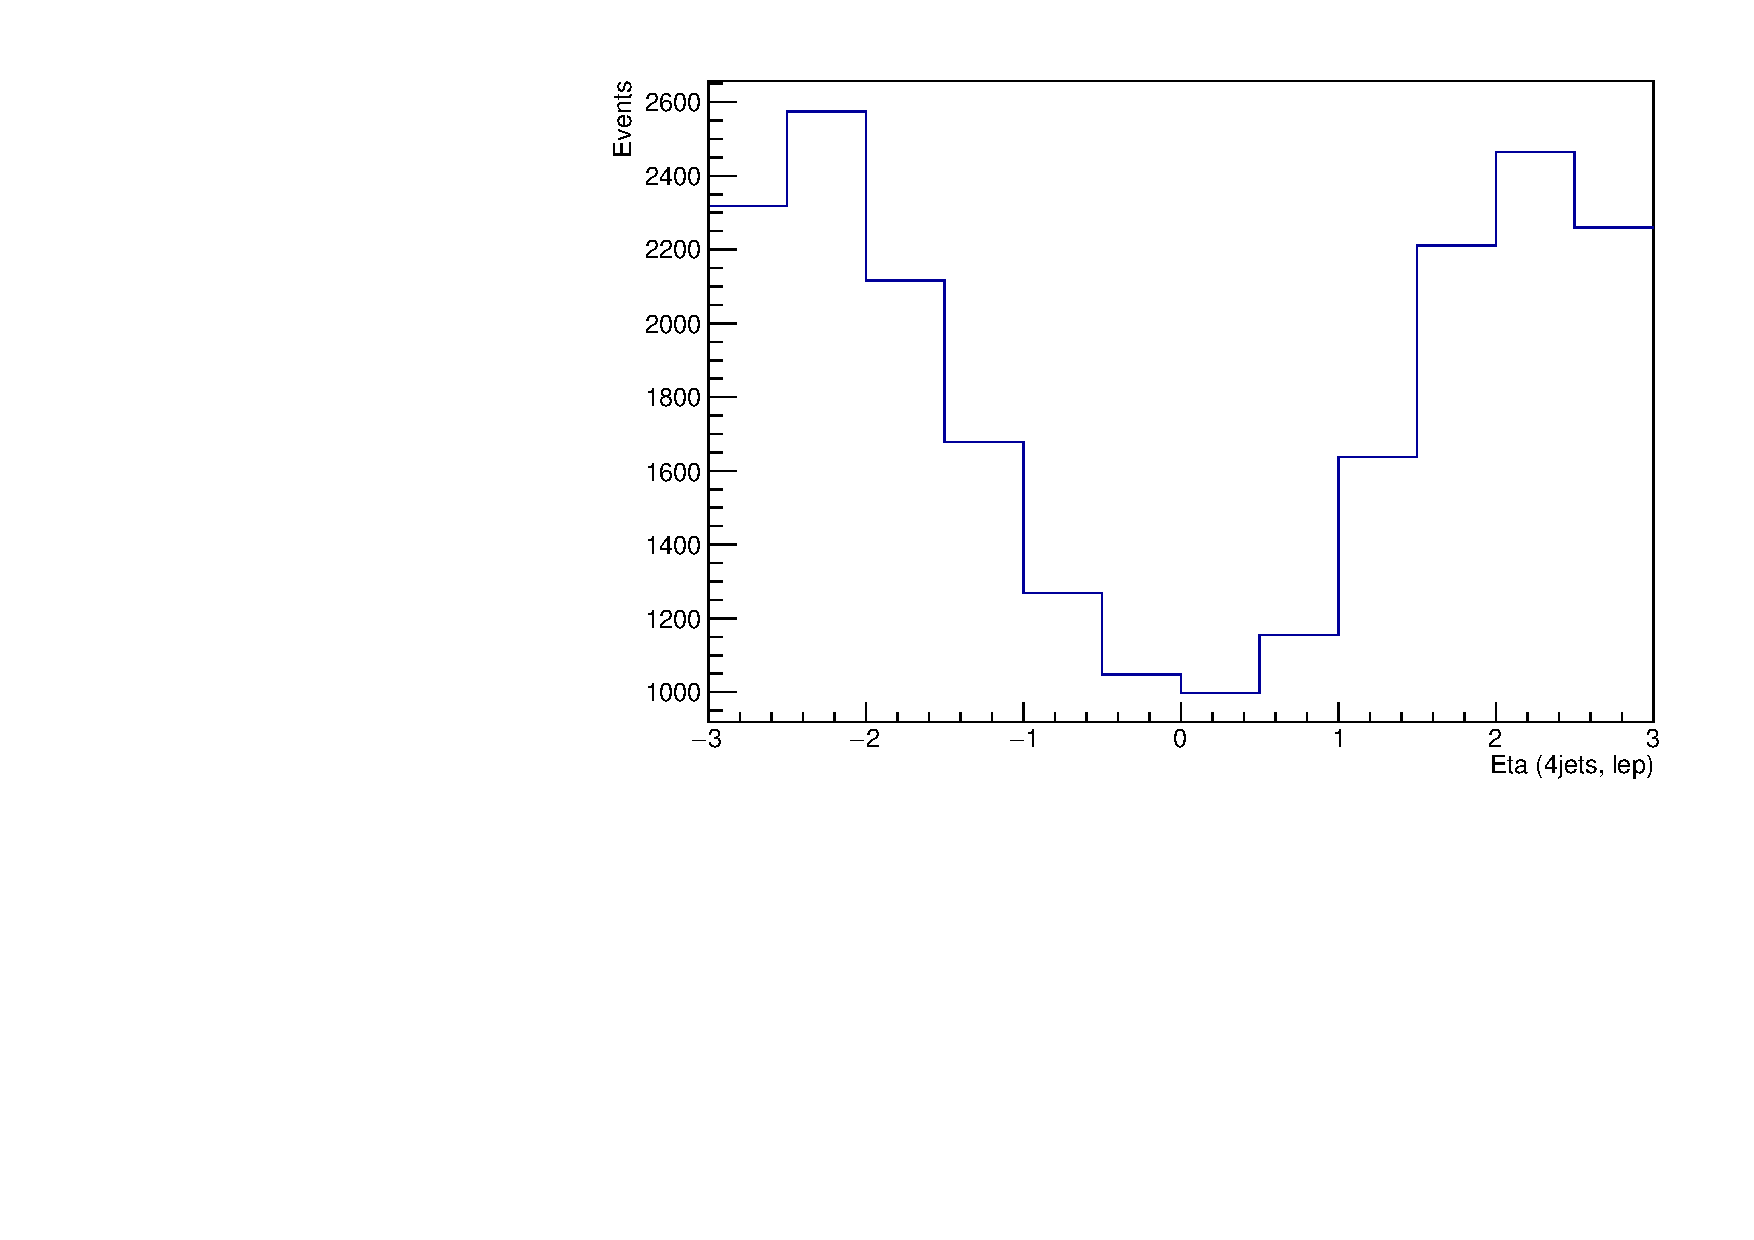
\includegraphics[width=\linewidth]{plots_and_txt/ttbar.mu_selected_/ttbar.mu_selected_FullSysEta.pdf}
    \caption{}
    \label{fig:ttbar_sys3}
  \end{subfigure}%
  \begin{subfigure}{0.5\textwidth}
    \centering
    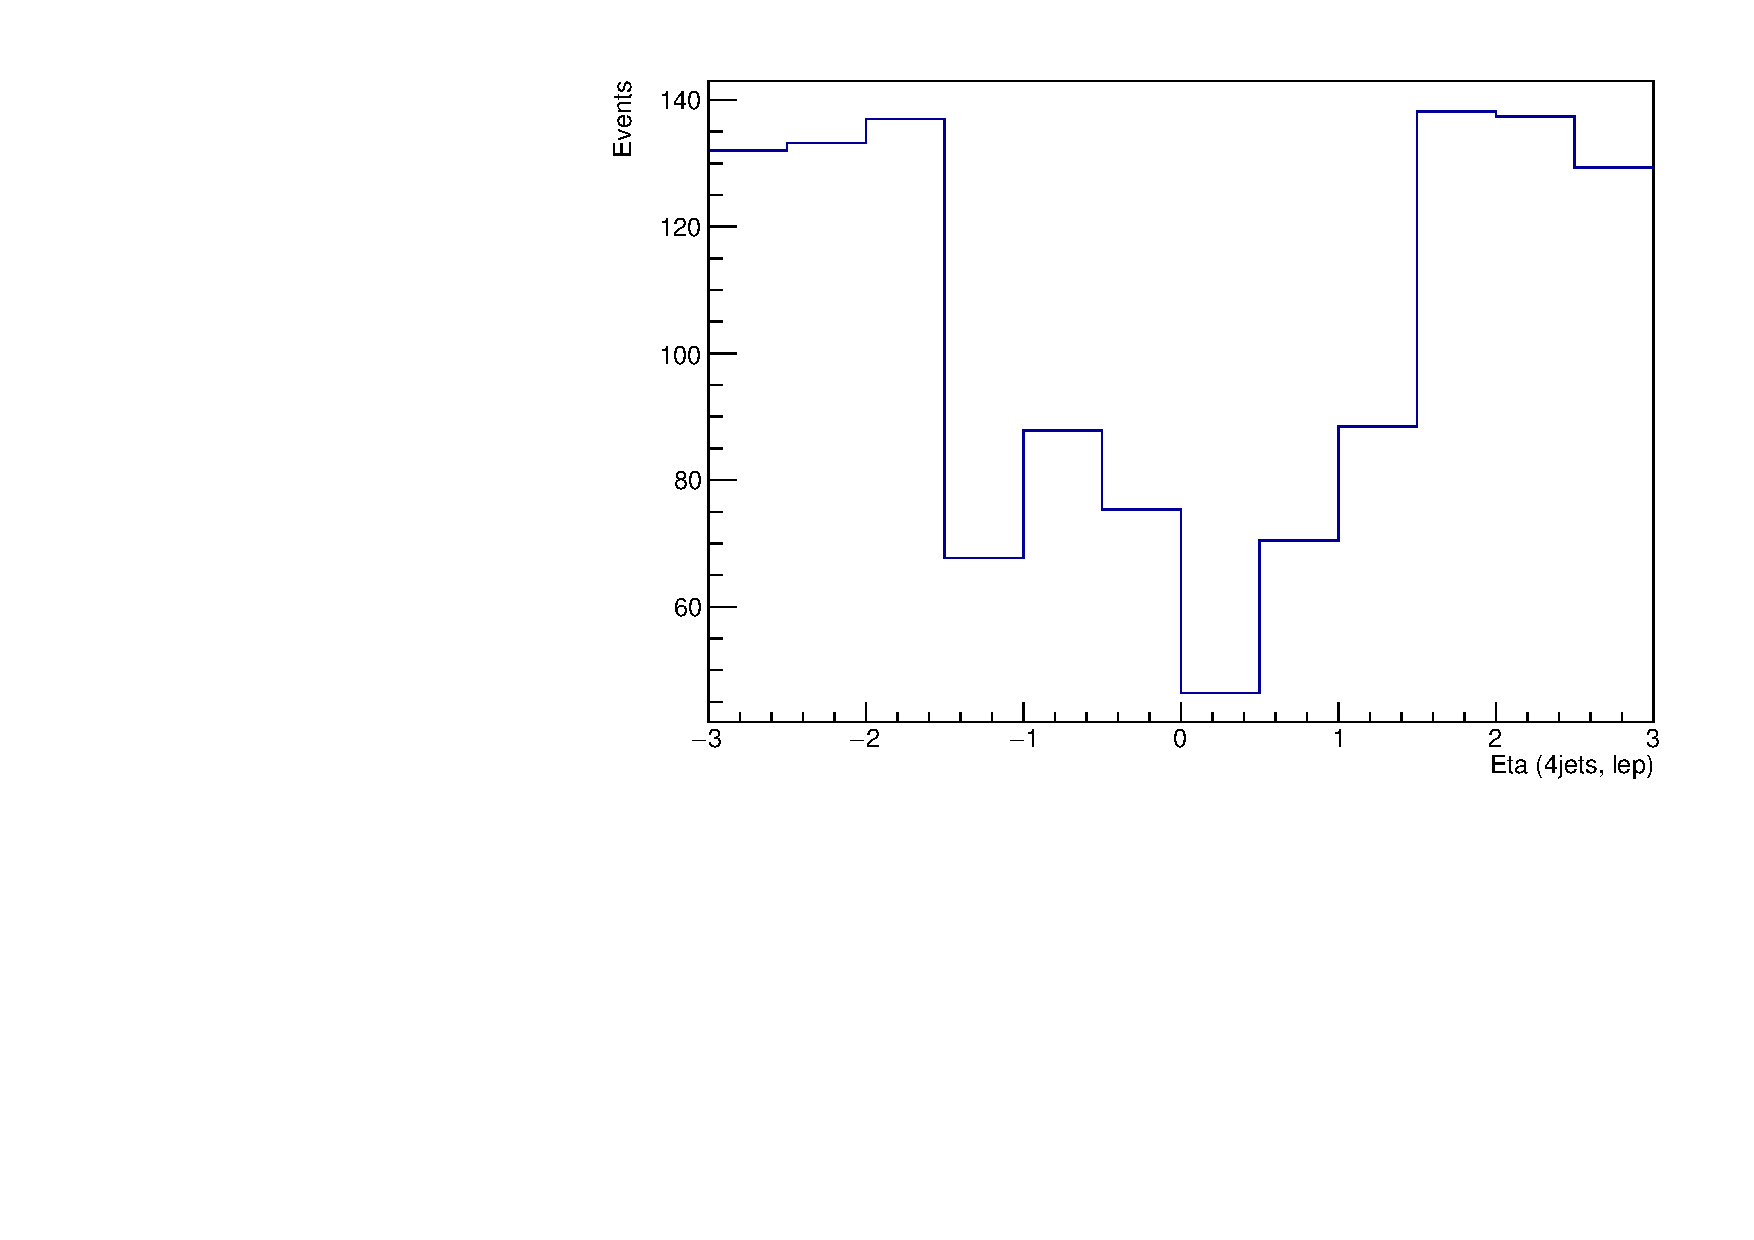
\includegraphics[width=\linewidth]{plots_and_txt/zprime1000.mu_selected_/zprime1000.mu_selected_FullSysEta.pdf}
    \caption{}
    \label{fig:zprime_sys3}
  \end{subfigure}%
  \caption{Vergleich der Verteilung der Pseudorapidität des Systems, die durch die vier Jets mit dem größten $p_T$, dem Lepton und dem Neutrino gebildet wird.
  Dies ist für die $t\bar{t}$-Untergrundsimulation \subref{fig:ttbar_sys3} und der Signalsimulation des $Z^\prime(1000)$ \subref{fig:zprime_sys3} dargestellt.
  }
  \label{fig:Comparison3}
\end{figure}



\subsection{Weitere Plots zur Überprüfung der Monte Carlo Übereinstimmung mit den 
Daten}
\label{sec:stackedrest}


\begin{figure}[H]
  \begin{subfigure}{0.5\textwidth}
    \centering
    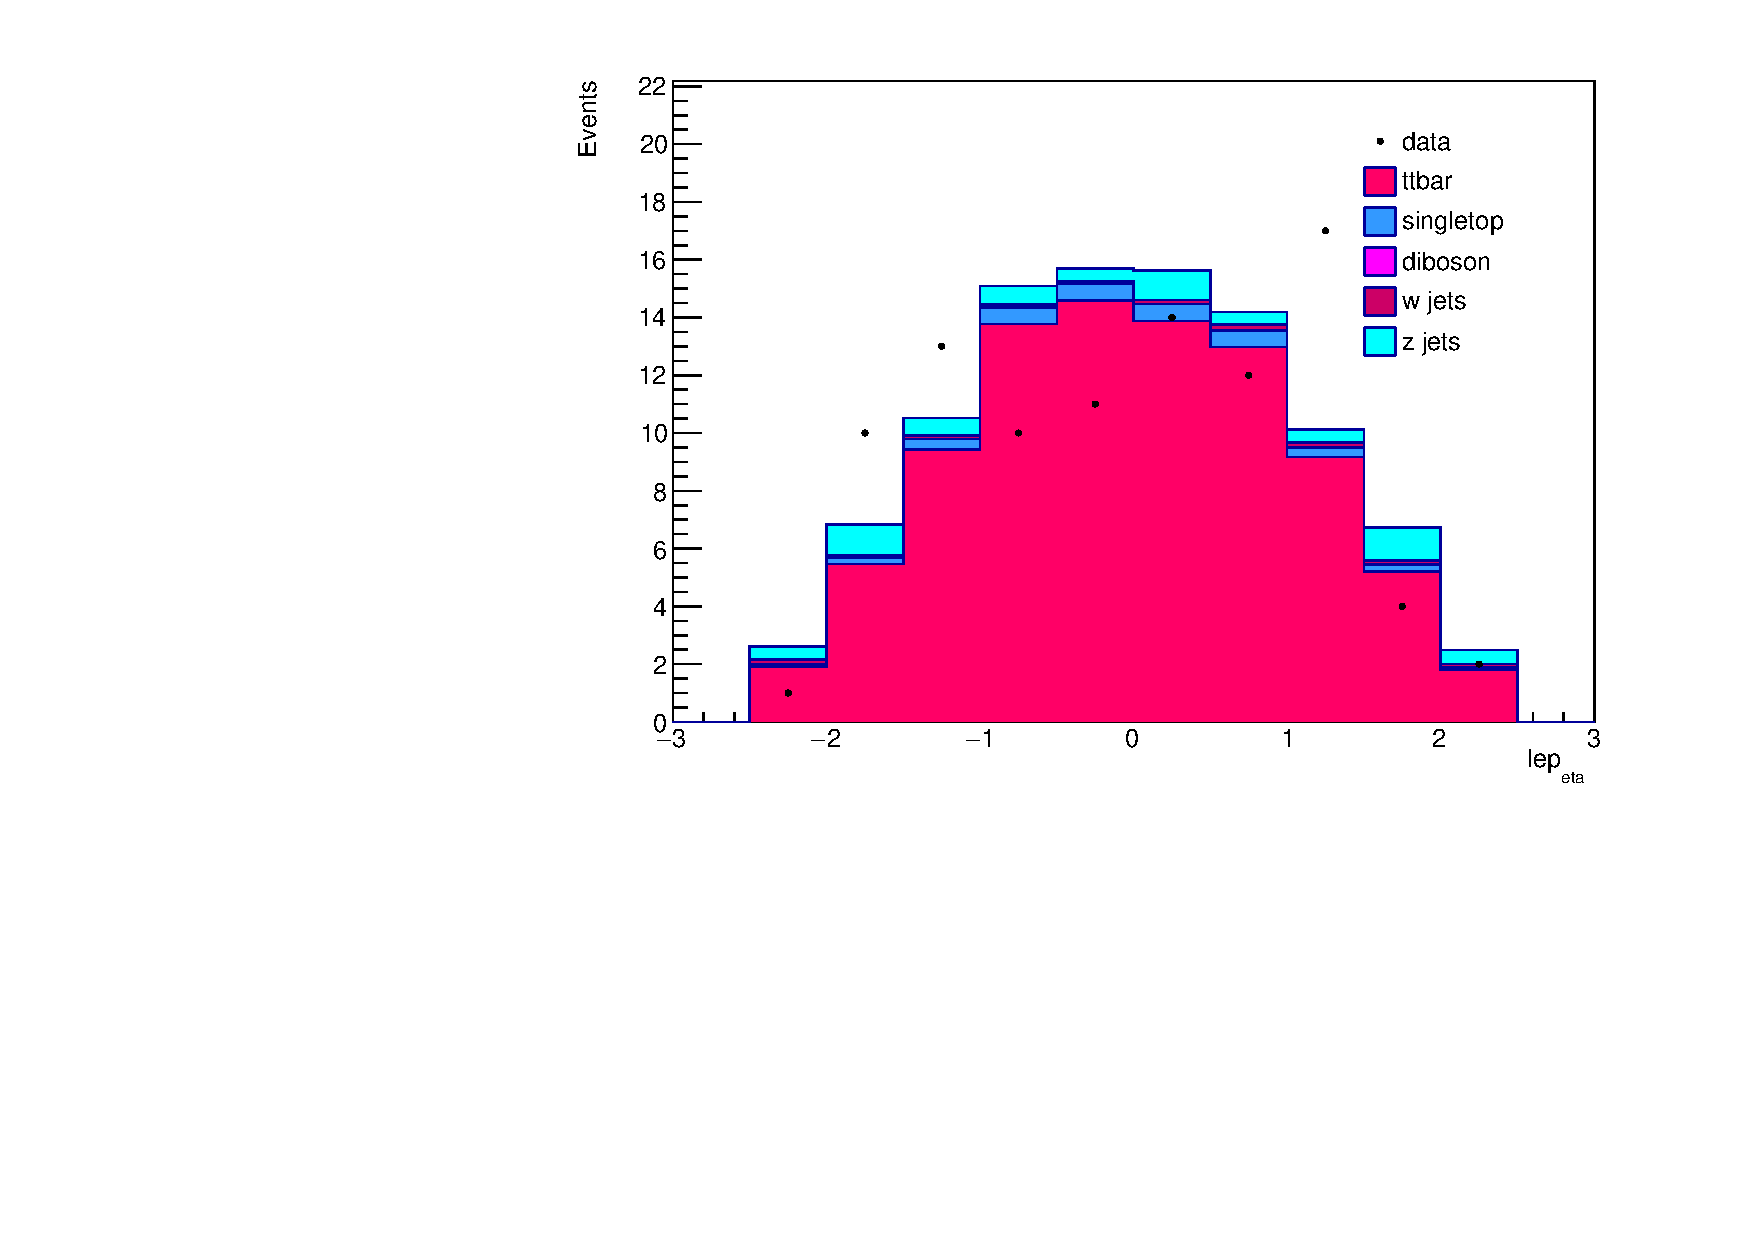
\includegraphics[width=\linewidth]{plots_and_txt/stacked_plots/stacked_lep_eta.pdf}
    \caption{}
    \label{fig:stacked_lep_pt2}
  \end{subfigure}%
  \begin{subfigure}{0.5\textwidth}
    \centering
    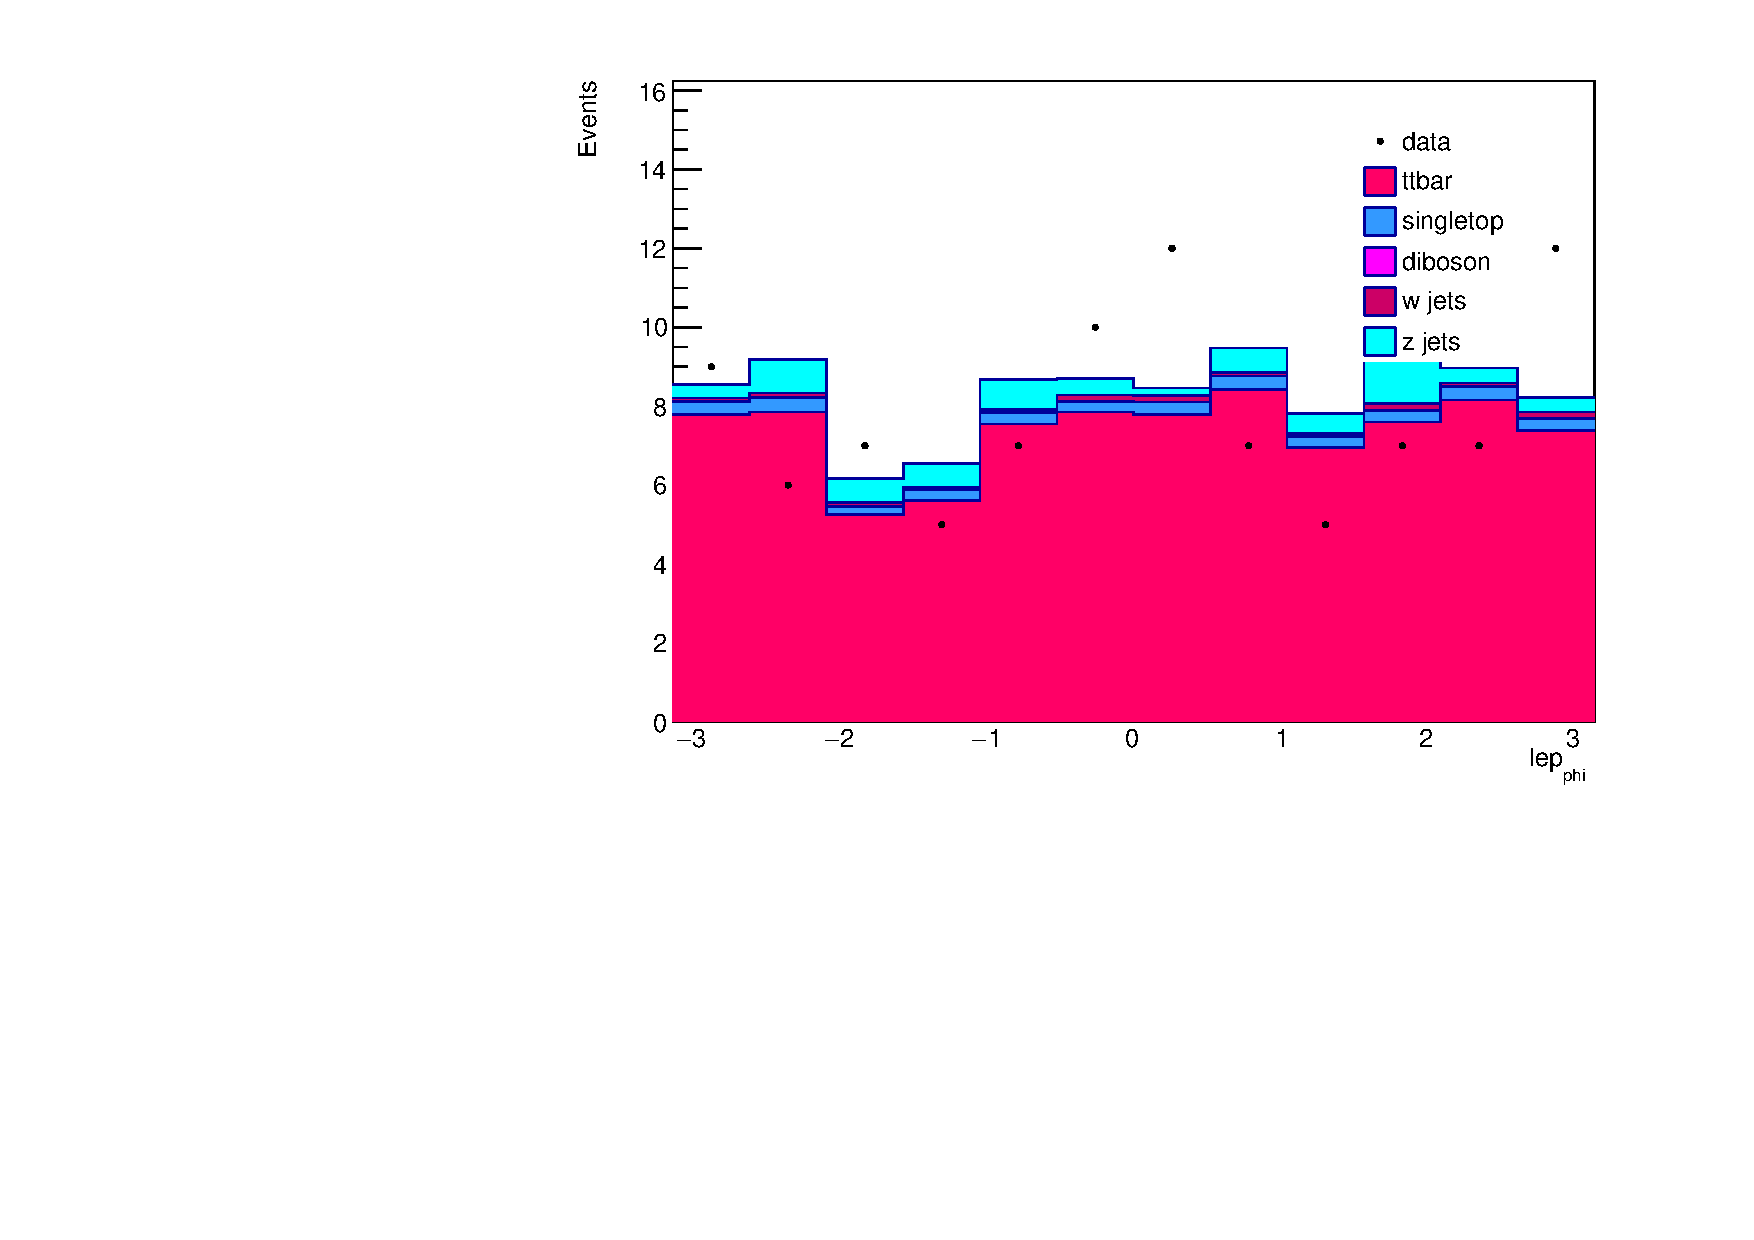
\includegraphics[width=\linewidth]{plots_and_txt/stacked_plots/stacked_lep_phi.pdf}
    \caption{}
    \label{fig:stacked_btagged2}
  \end{subfigure}%
  \newline
  \begin{subfigure}{0.5\textwidth}
    \centering
    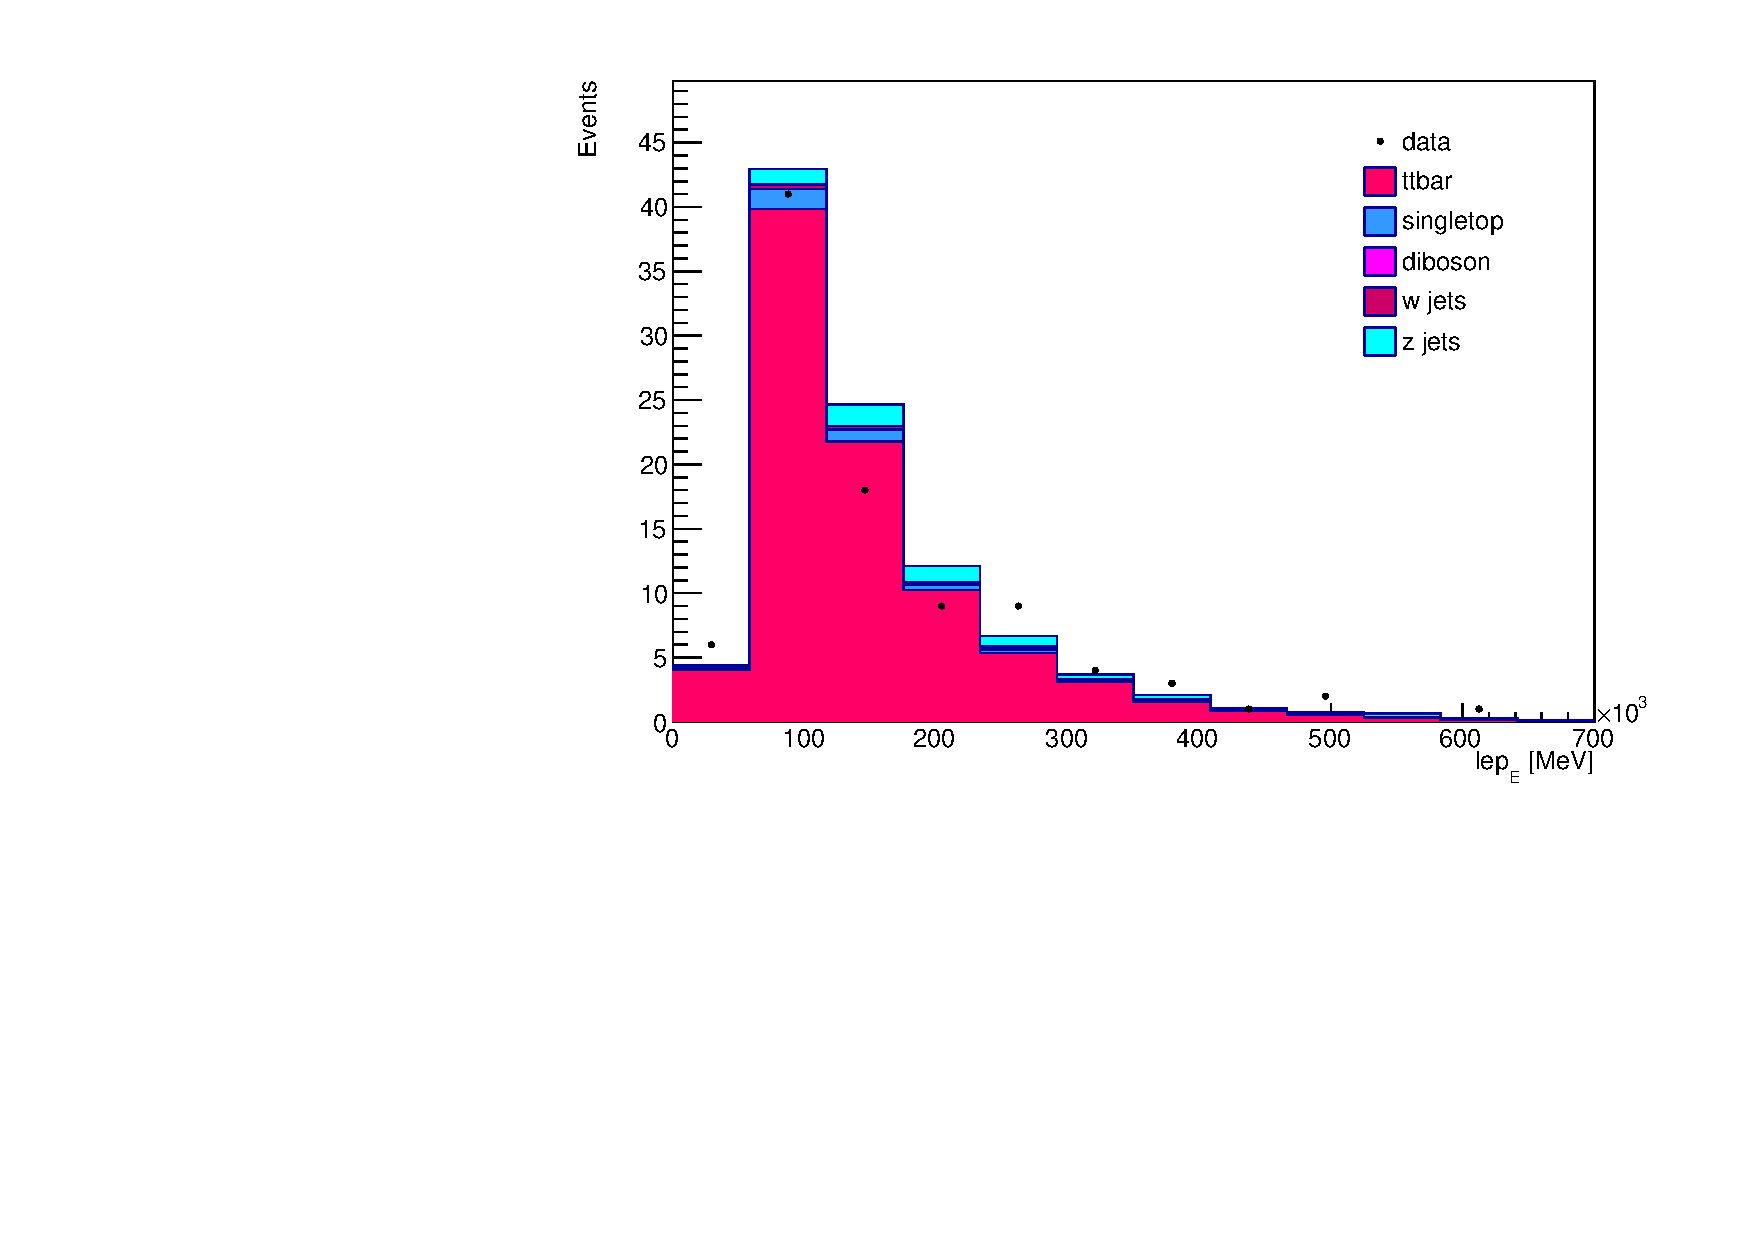
\includegraphics[width=\linewidth]{plots_and_txt/stacked_plots/stacked_lep_E.pdf}
    \caption{}
    \label{fig:stacked_jet_pt_good2}
  \end{subfigure}%
  \begin{subfigure}{0.5\textwidth}
    \centering
    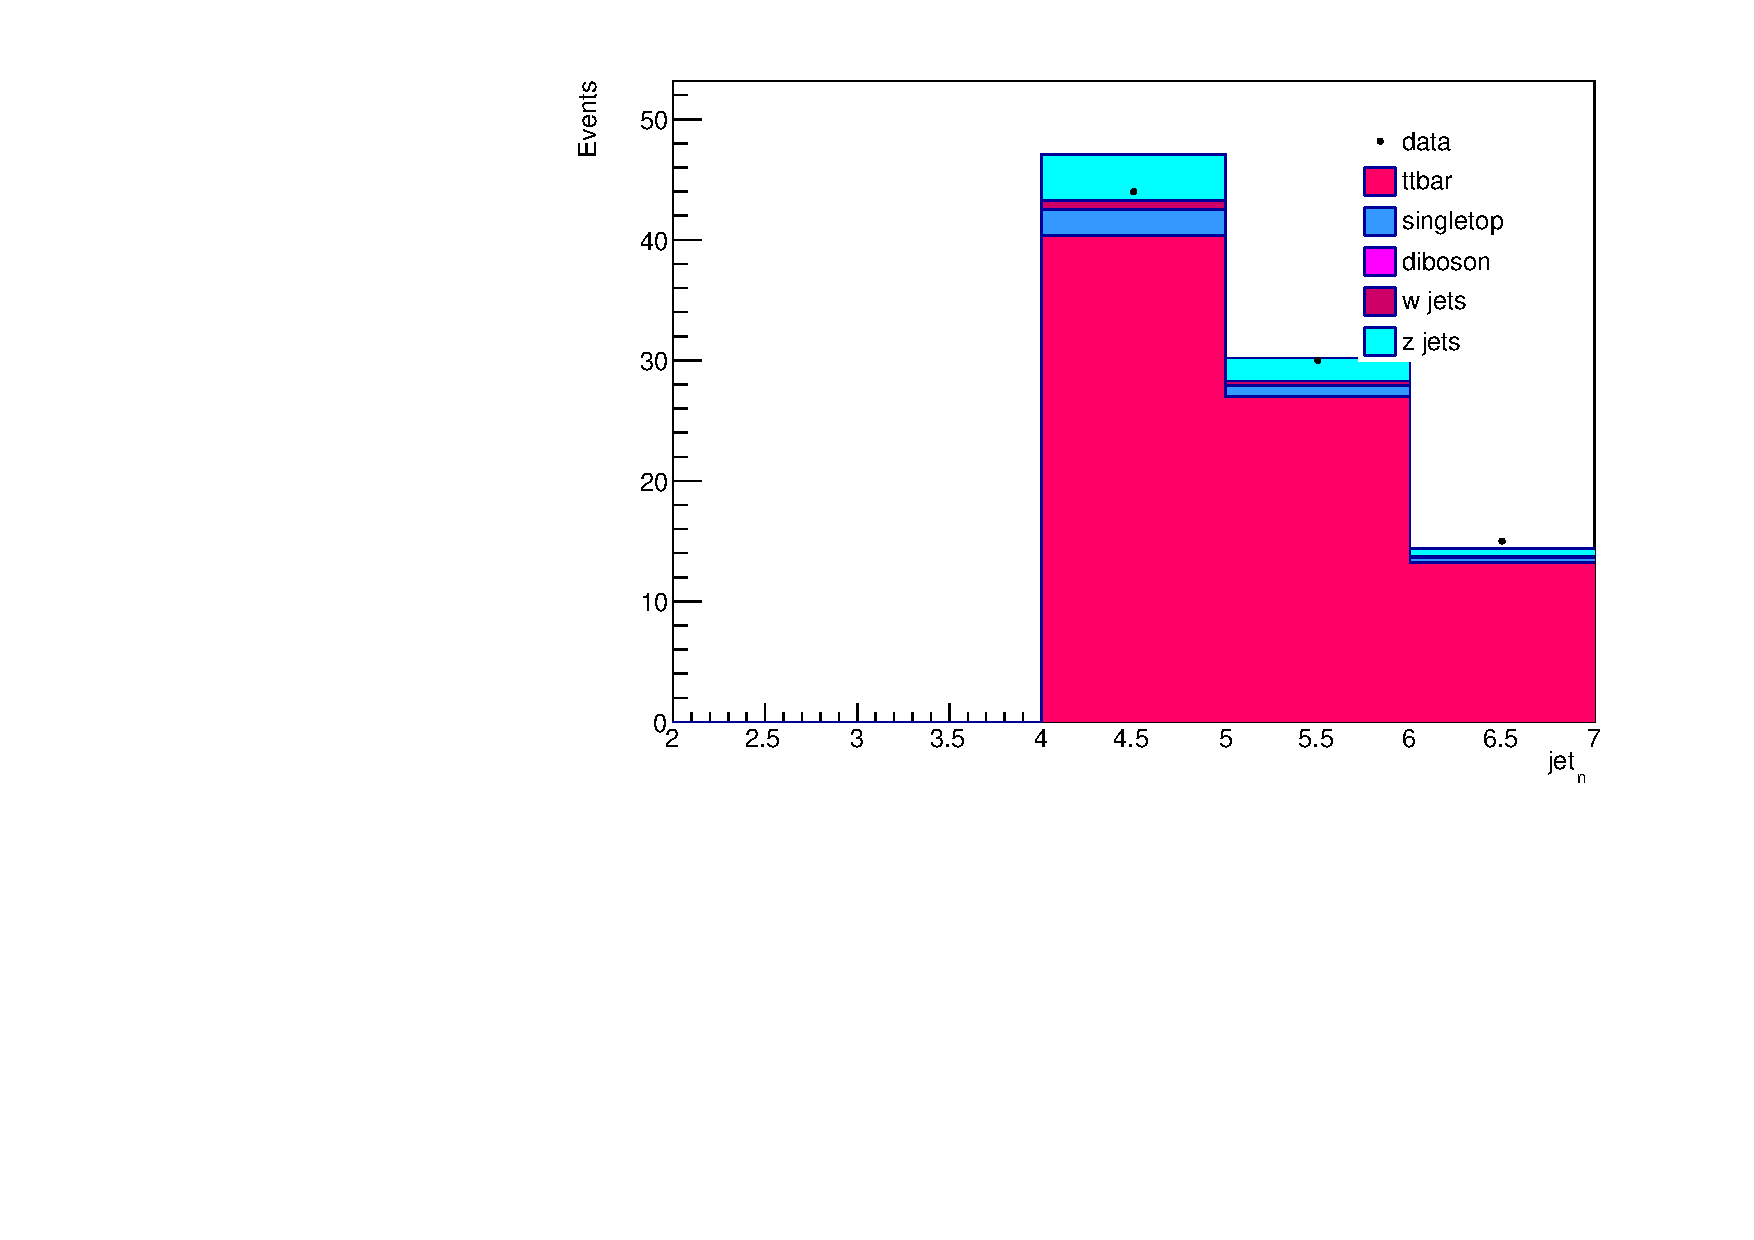
\includegraphics[width=\linewidth]{plots_and_txt/stacked_plots/stacked_jet_n.pdf}
    \caption{}
    \label{fig:stacked_met_et2}
  \end{subfigure}%
  \caption{Darstellung verschiedener Verteilungen der Größen der $t\bar{t}$ Monte-Carlo Simulation.
  Zusehen sind die Pseudorapidität der Myonen (\subref{fig:stacked_lep_pt2}), 
  der Azimuthalwinkel der Leptonen (\subref{fig:stacked_btagged2}), 
  der Energie der Myonen (\subref{fig:stacked_jet_pt_good2}) und die Anzahl an nutzbaren Jets (\subref{fig:stacked_met_et2}).
  }
  \label{fig:stacked_Distributions2}
\end{figure}

\begin{figure}[H]
  \begin{subfigure}{0.5\textwidth}
    \centering
    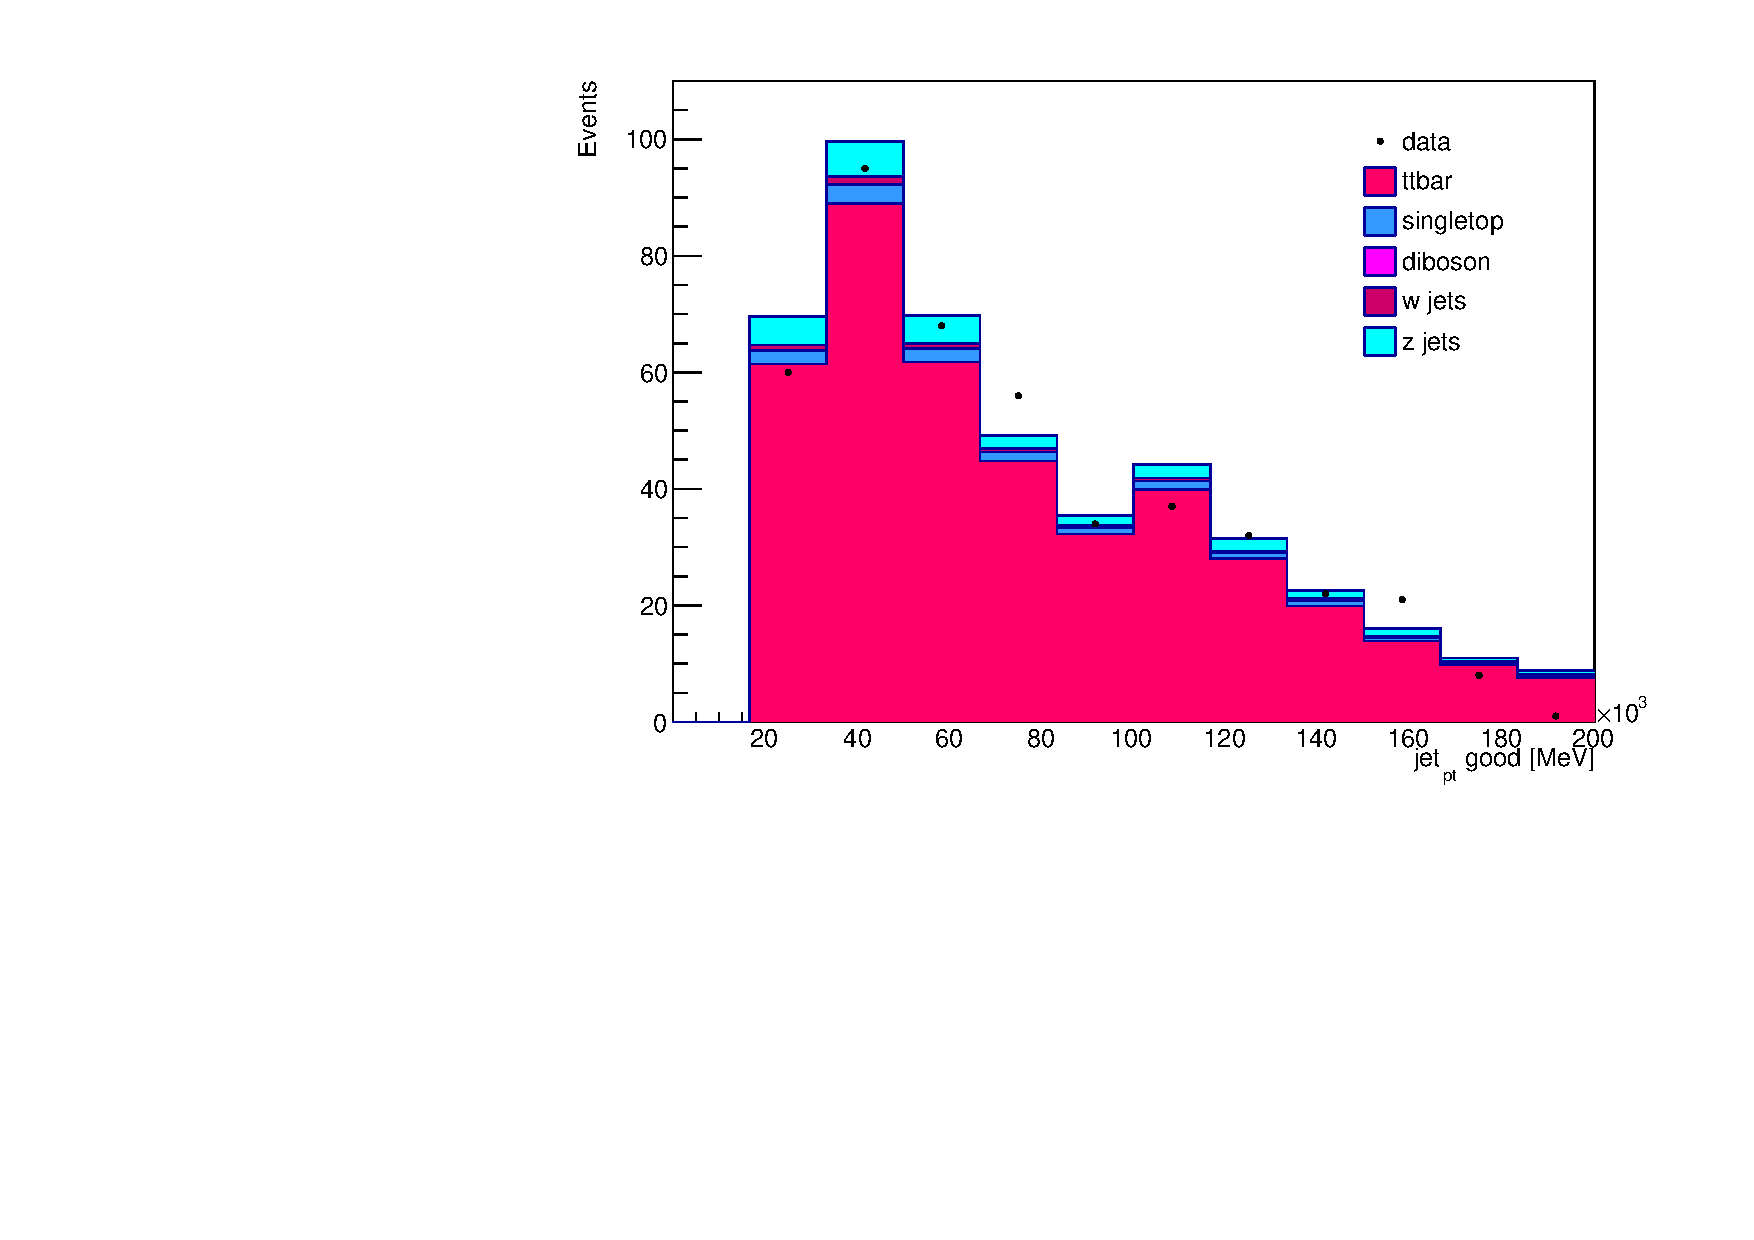
\includegraphics[width=\linewidth]{plots_and_txt/stacked_plots/stacked_jet_pt_good.pdf}
    \caption{}
    \label{fig:stacked_lep_pt3}
  \end{subfigure}%
  \begin{subfigure}{0.5\textwidth}
    \centering
    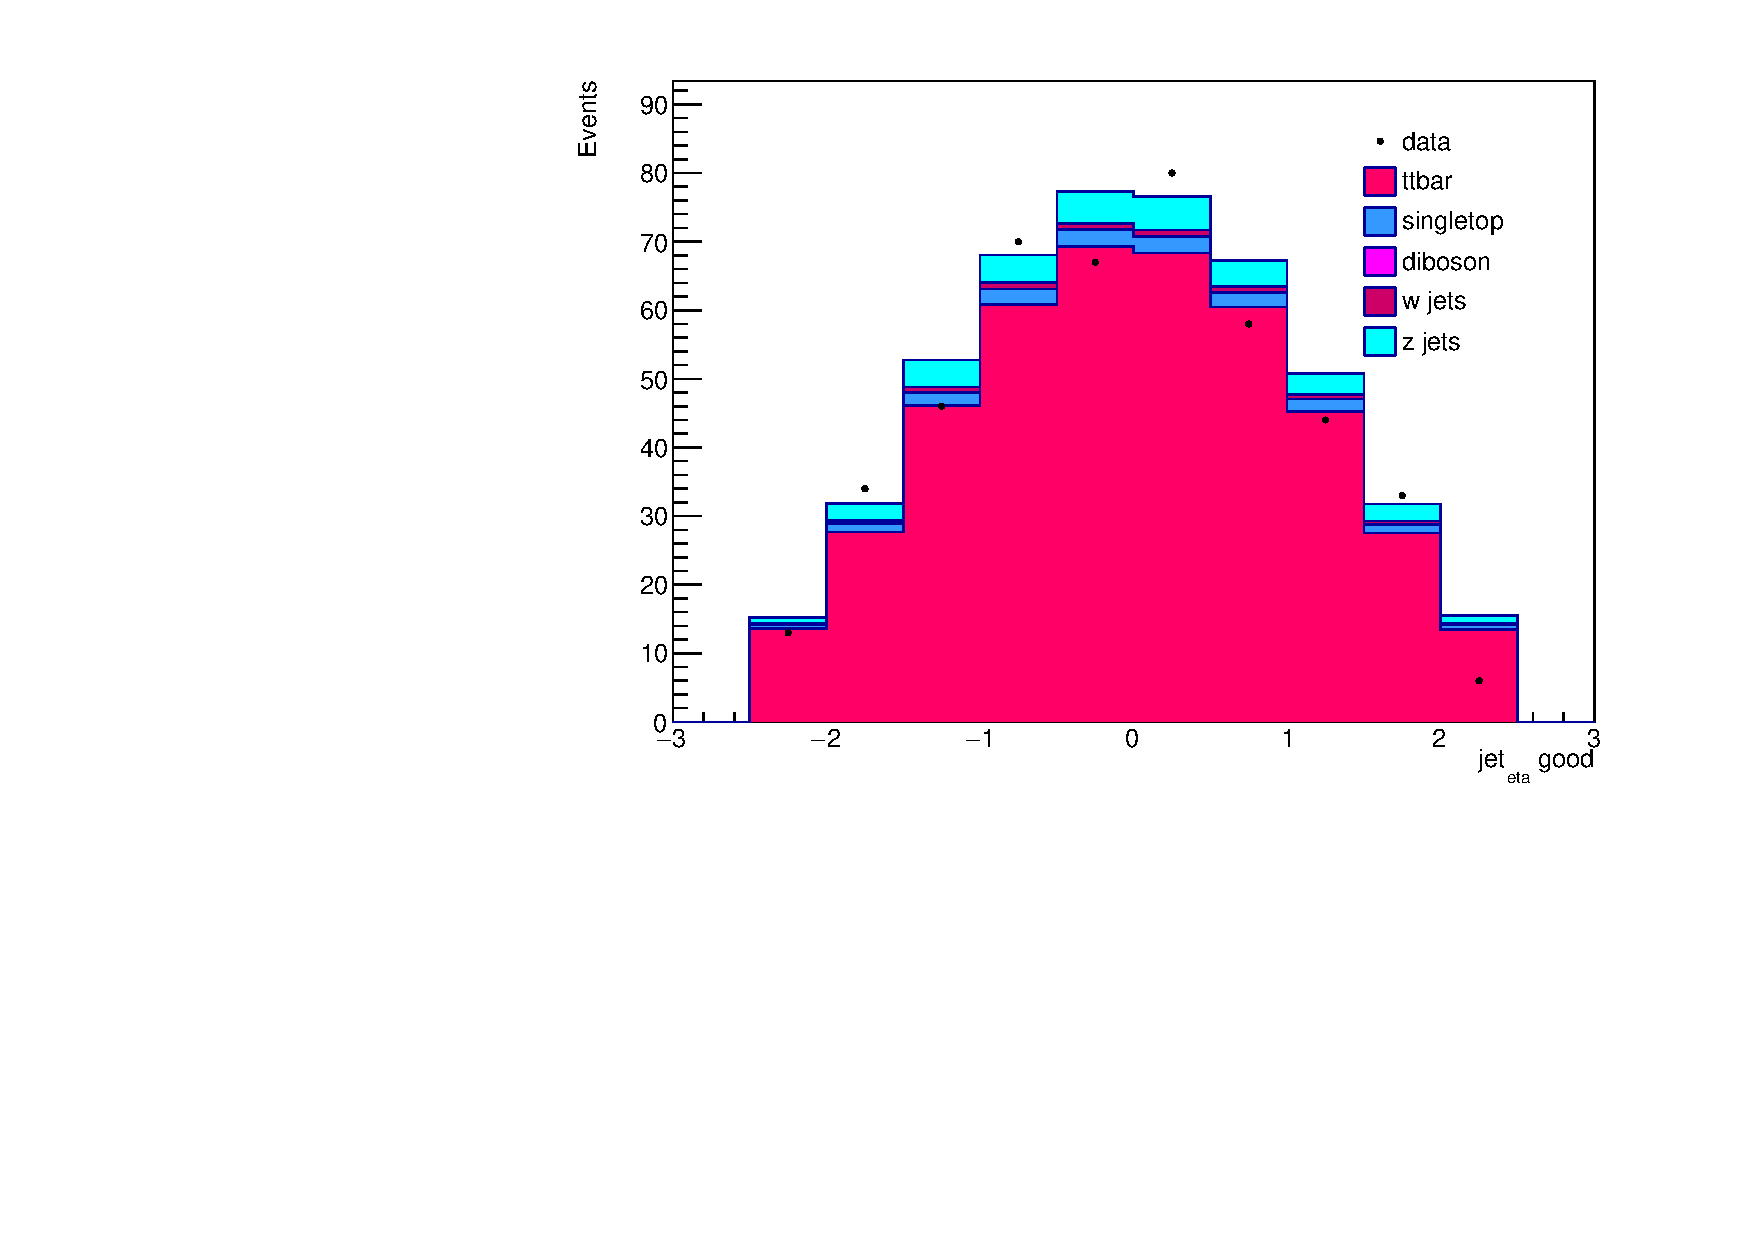
\includegraphics[width=\linewidth]{plots_and_txt/stacked_plots/stacked_jet_eta_good.pdf}
    \caption{}
    \label{fig:stacked_btagged3}
  \end{subfigure}%
  \newline
  \begin{subfigure}{0.5\textwidth}
    \centering
    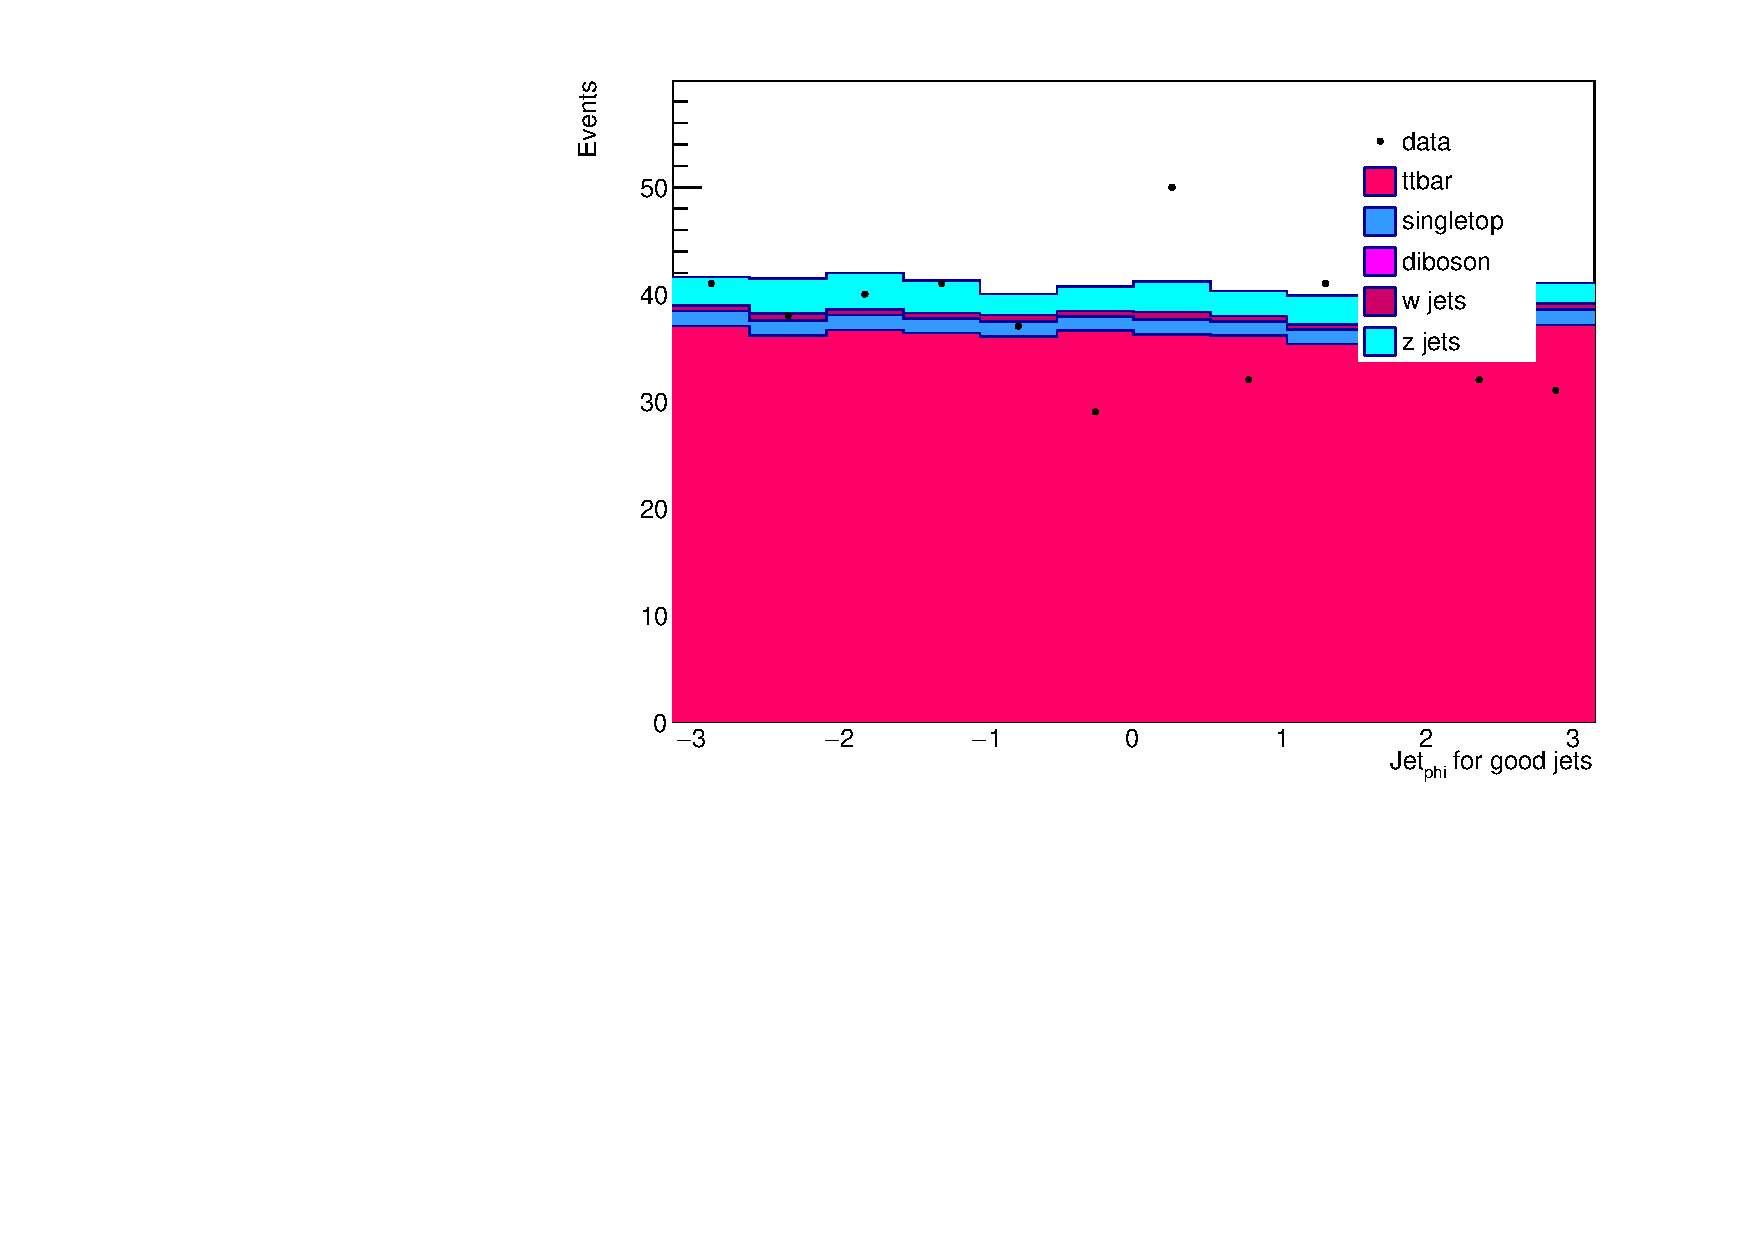
\includegraphics[width=\linewidth]{plots_and_txt/stacked_plots/stacked_jet_phi_good.pdf}
    \caption{}
    \label{fig:stacked_jet_pt_good3}
  \end{subfigure}%
  \begin{subfigure}{0.5\textwidth}
    \centering
    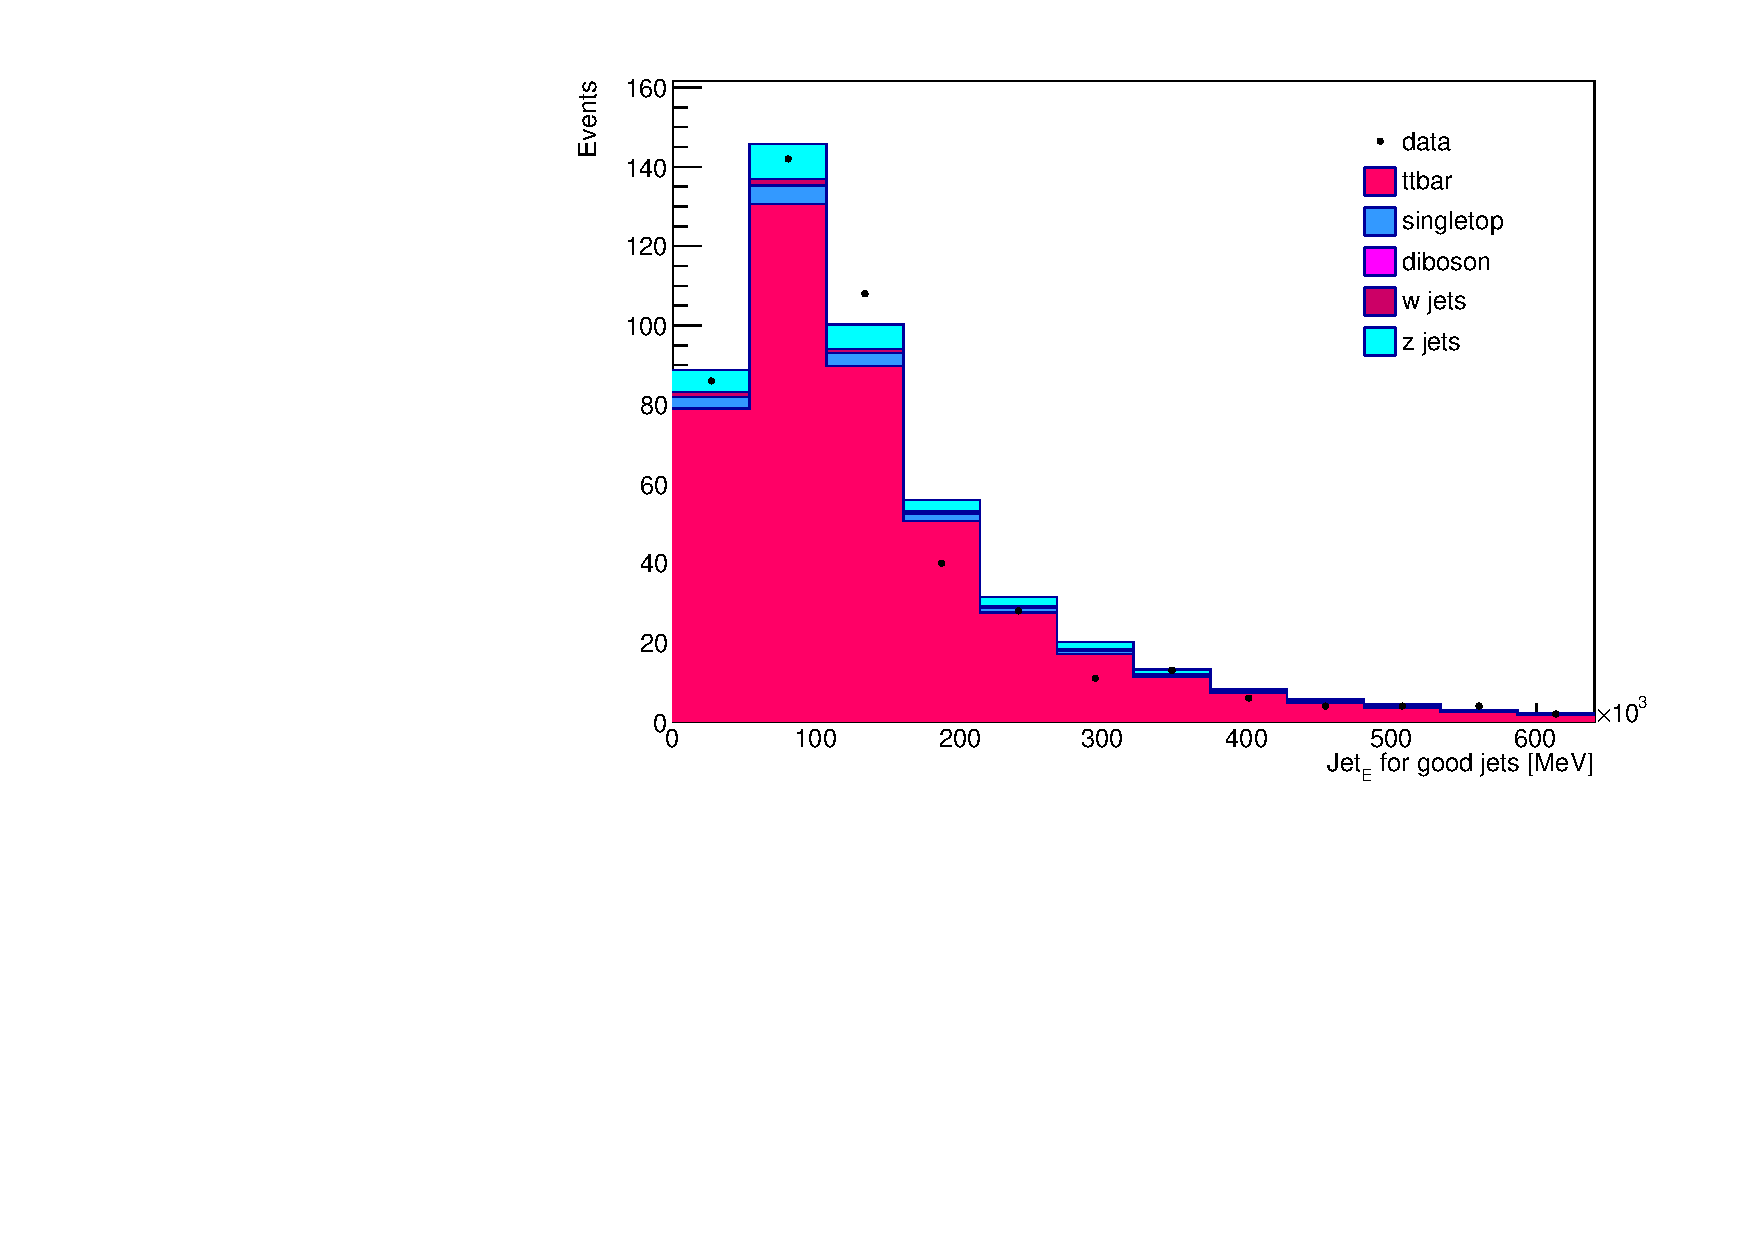
\includegraphics[width=\linewidth]{plots_and_txt/stacked_plots/stacked_jet_E_good.pdf}
    \caption{}
    \label{fig:stacked_met_et3}
  \end{subfigure}%
  \caption{Darstellung verschiedener Verteilungen der Größen der $t\bar{t}$ Monte-Carlo Simulation.
  Zusehen sind der transverale Impuls der nutzbaren Jets (\subref{fig:stacked_lep_pt3}), 
  die Pseudorapidität der nutzbaren Jets (\subref{fig:stacked_btagged3}), der Azimuthalwinkel der nutzbaren Jets (\subref{fig:stacked_jet_pt_good3}) 
  und die Energie der nutzbaren Jets (\subref{fig:stacked_met_et3}).
  }
  \label{fig:stacked_Distributions3}
\end{figure}

\begin{figure}[H]
  \begin{subfigure}{0.5\textwidth}
    \centering
    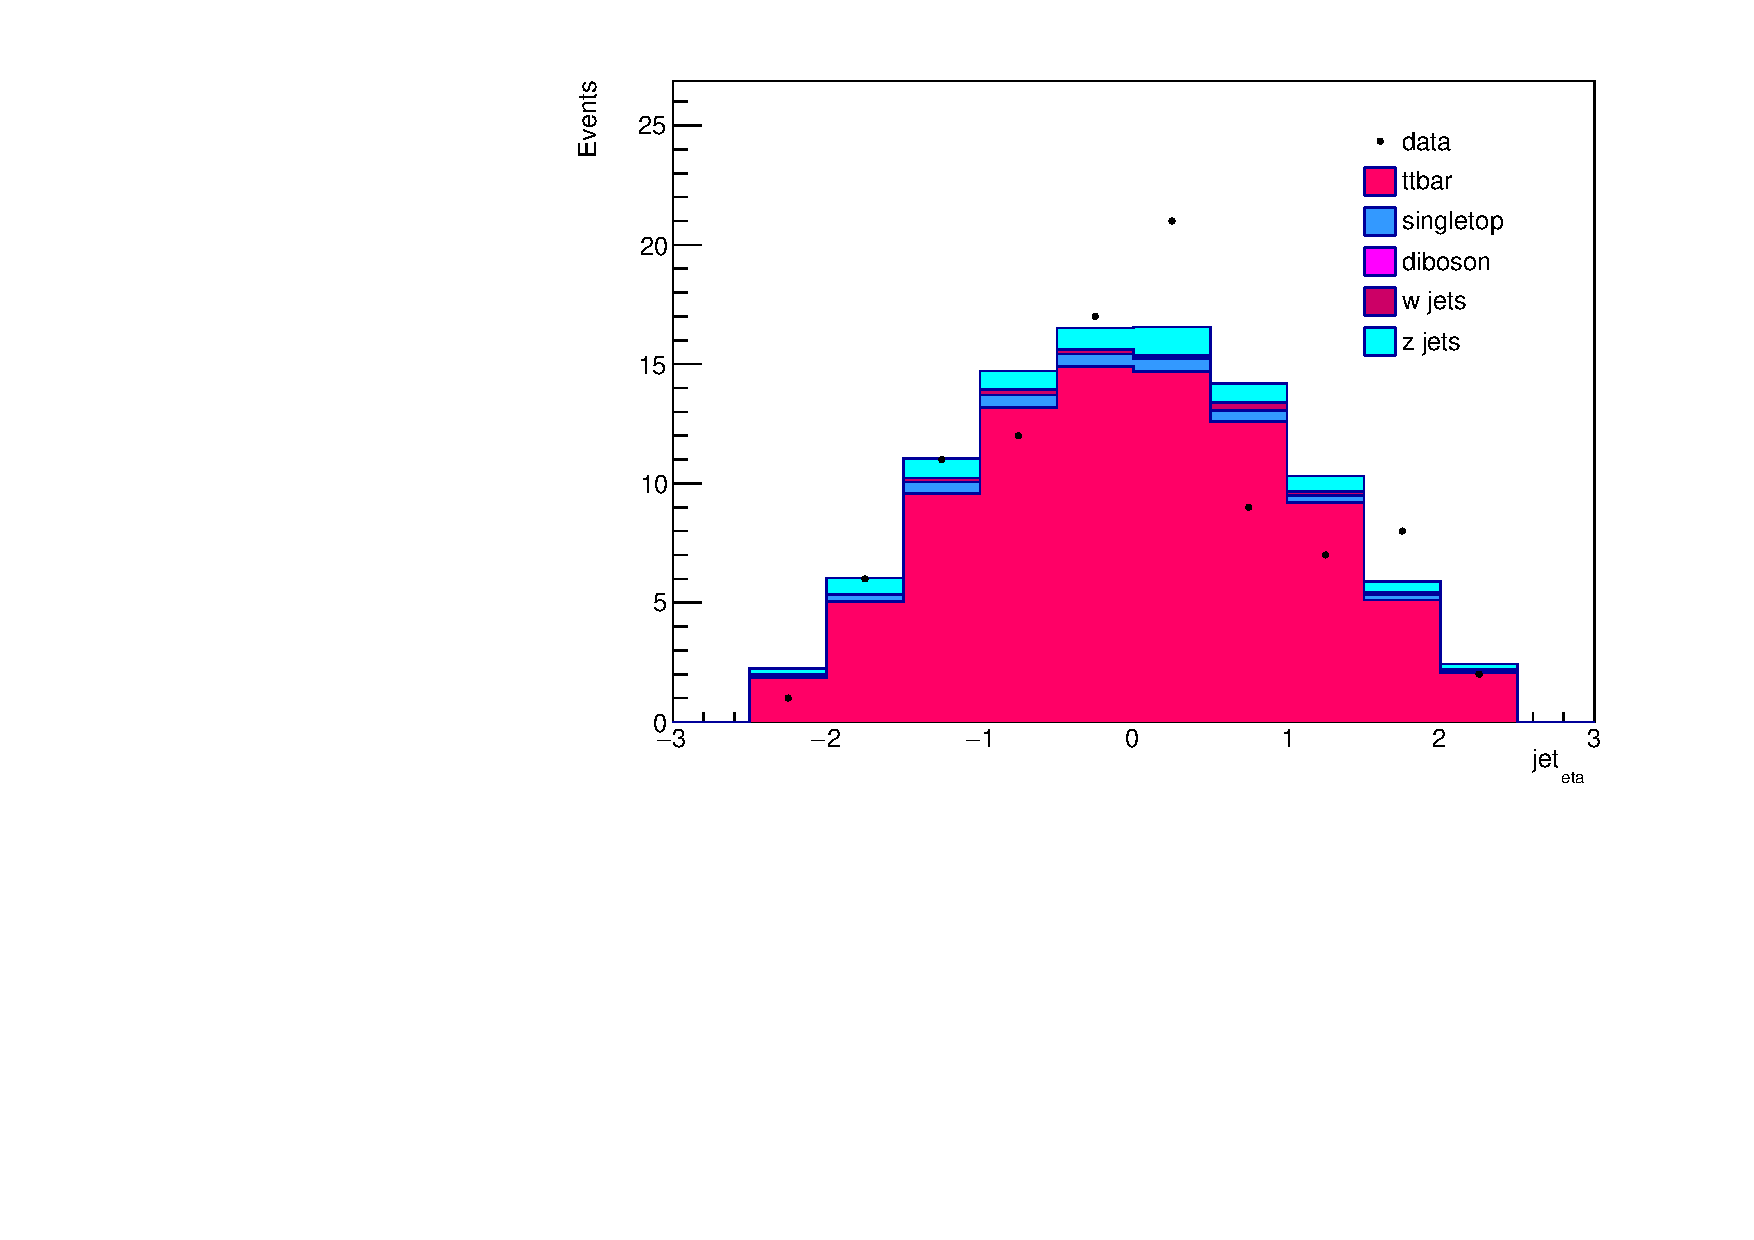
\includegraphics[width=\linewidth]{plots_and_txt/stacked_plots/stacked_jet_eta.pdf}
    \caption{}
    \label{fig:stacked_lep_pt4}
  \end{subfigure}%
  \begin{subfigure}{0.5\textwidth}
    \centering
    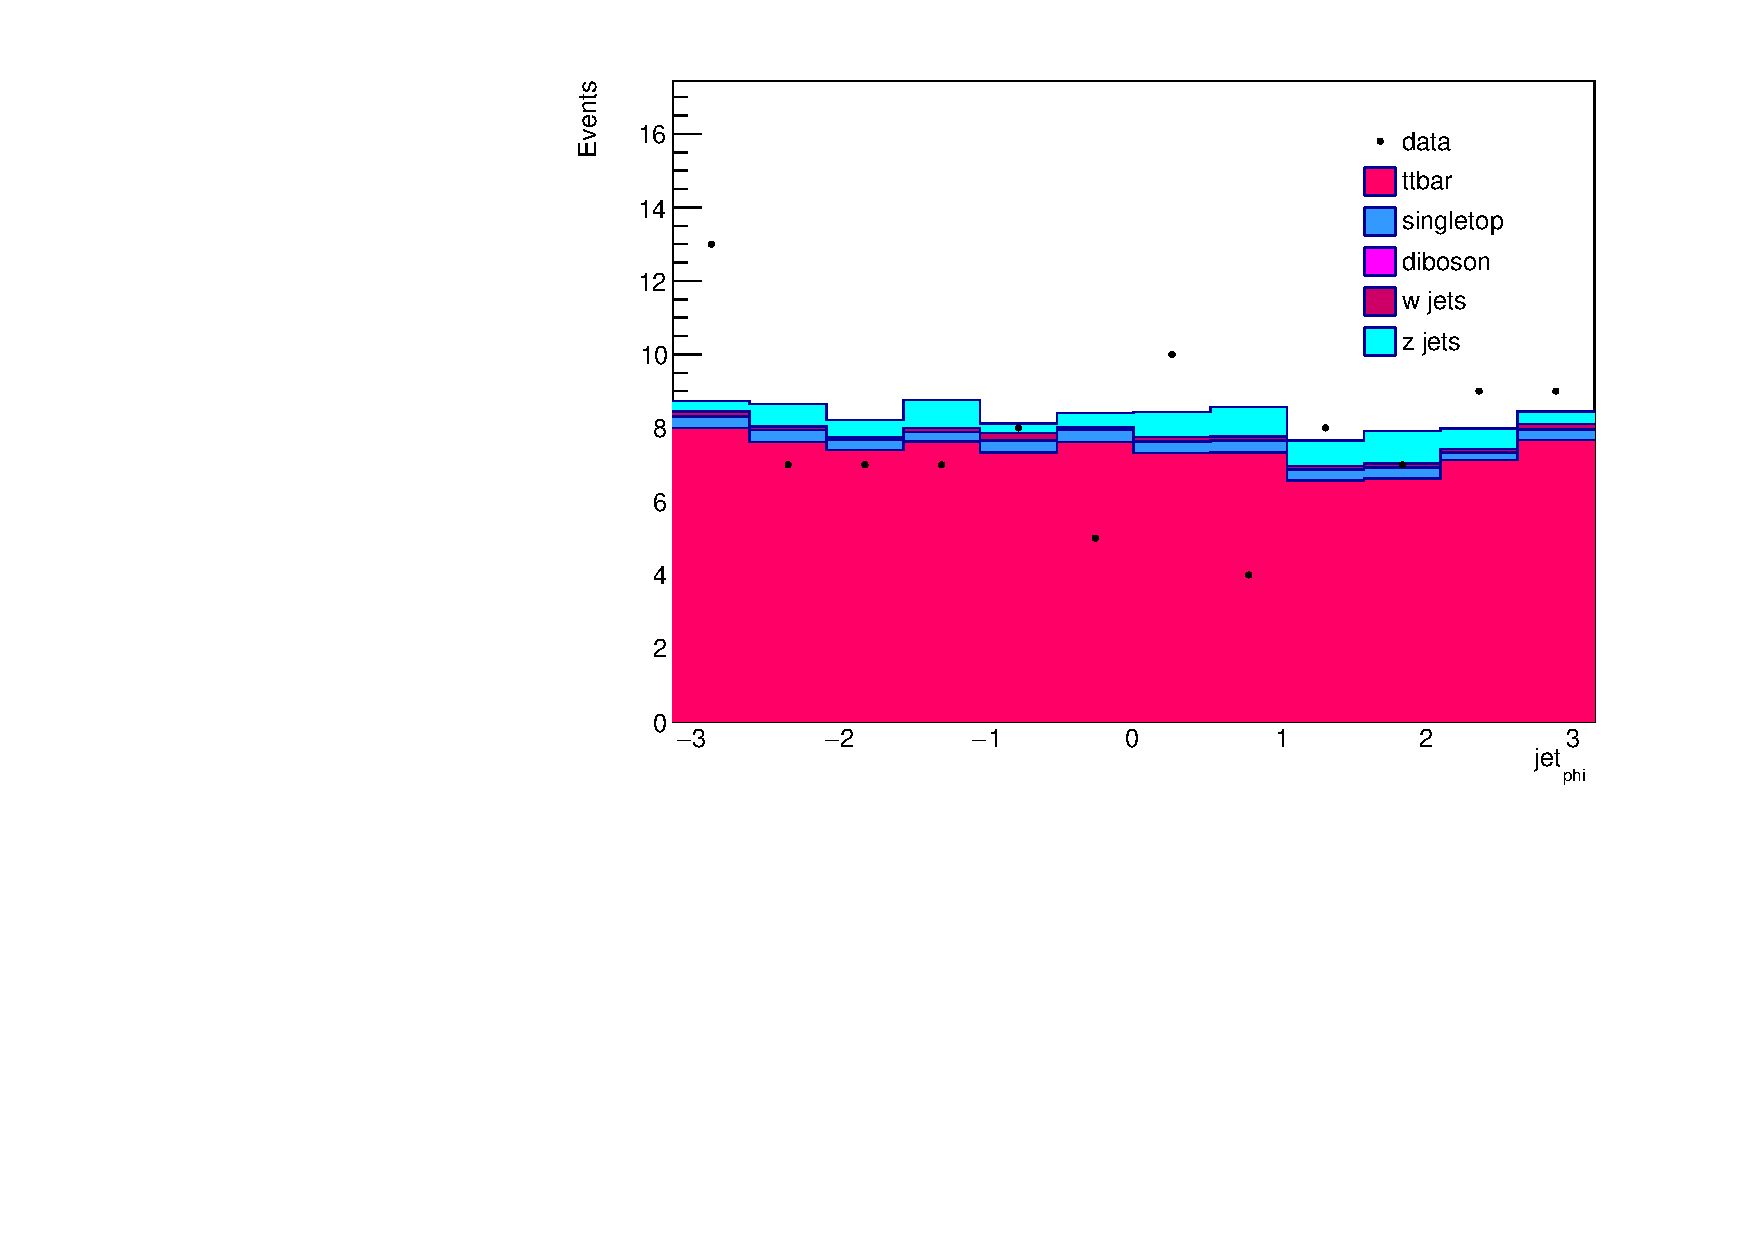
\includegraphics[width=\linewidth]{plots_and_txt/stacked_plots/stacked_jet_phi.pdf}
    \caption{}
    \label{fig:stacked_btagged4}
  \end{subfigure}%
  \newline
  \begin{subfigure}{0.5\textwidth}
    \centering
    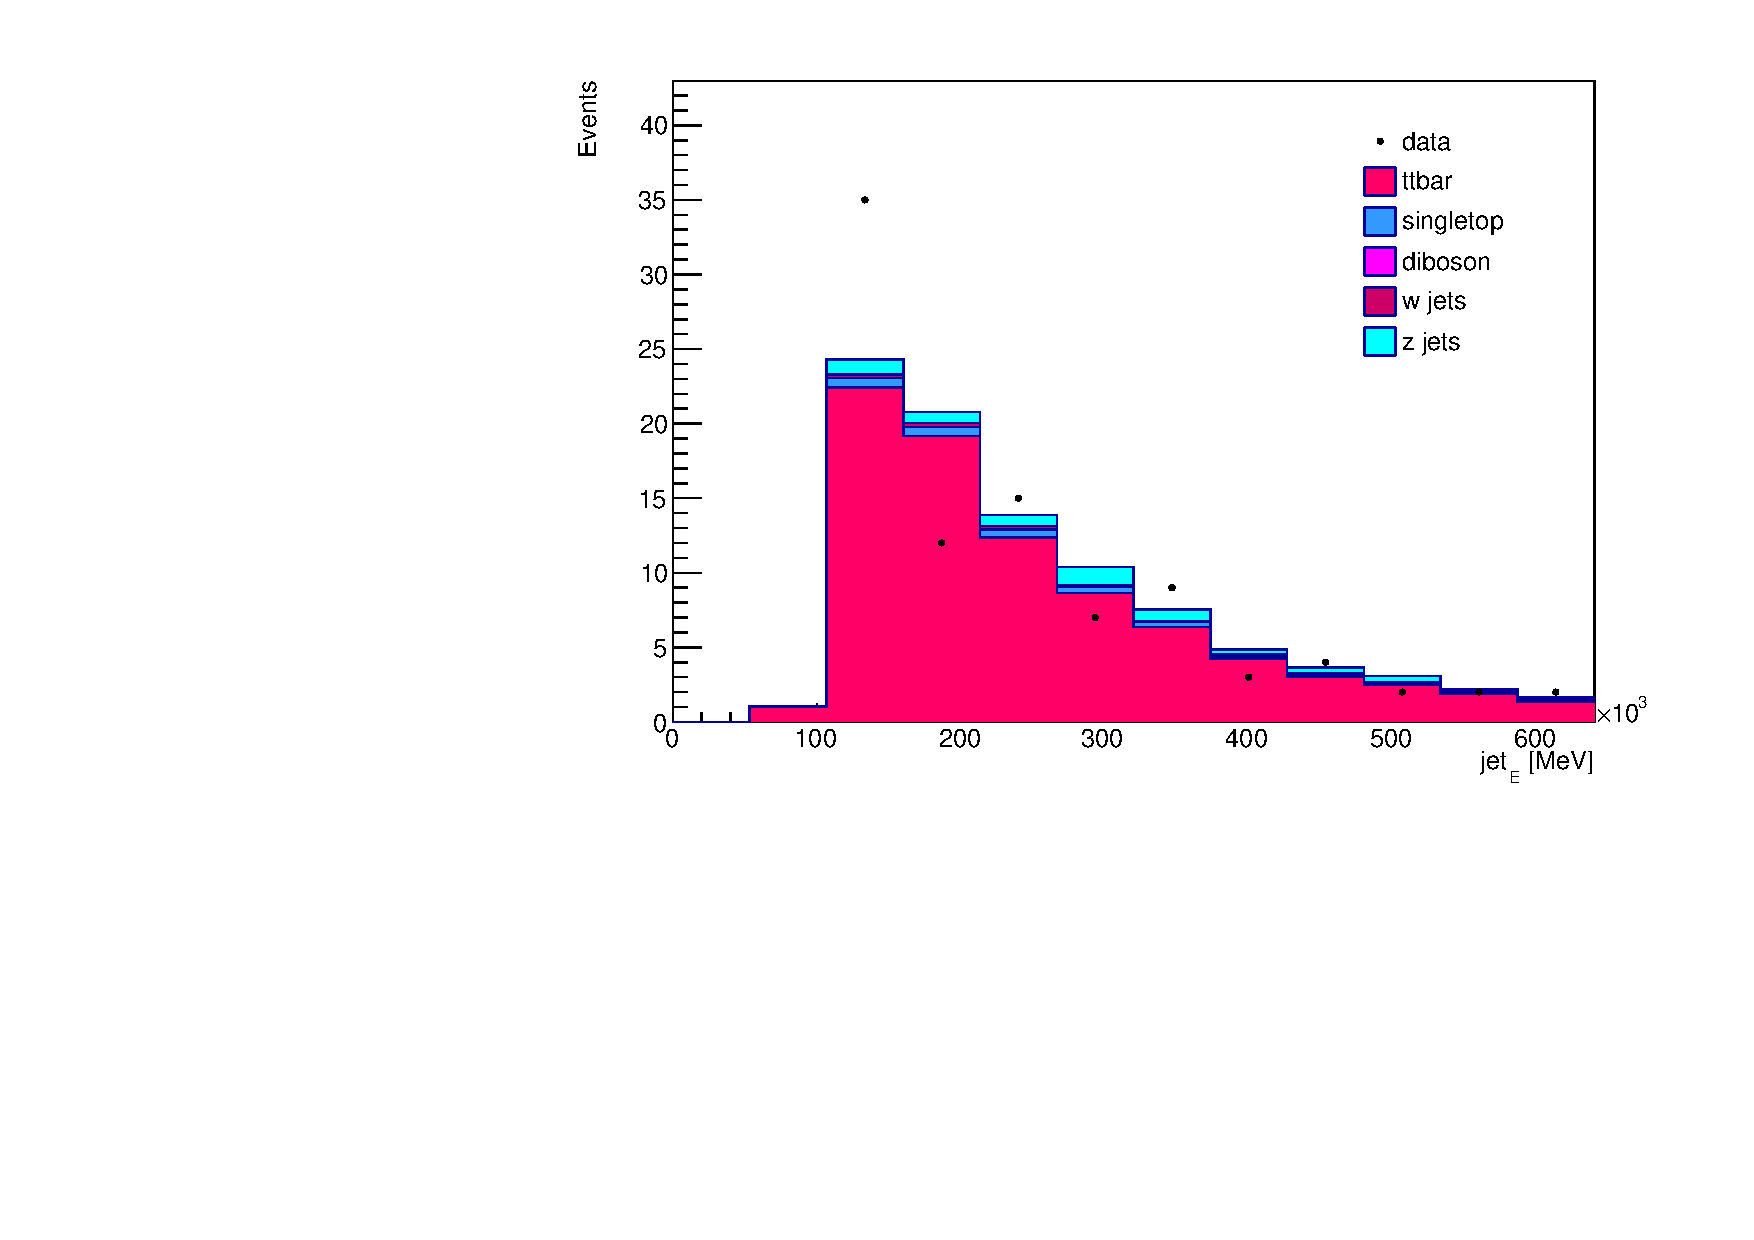
\includegraphics[width=\linewidth]{plots_and_txt/stacked_plots/stacked_jet_E.pdf}
    \caption{}
    \label{fig:stacked_jet_pt_good4}
  \end{subfigure}%
  \caption{Darstellung verschiedener Stacked Plots als Überprüfung der Übereinstimmung von Simulation und Daten.
  Zusehen sind die Pseudorapidität des Jets mit dem höchsten $p_T$ (\subref{fig:stacked_lep_pt4}),  
  der Azimuthalwinkel des Jets mit dem höchsten $p_T$ (\subref{fig:stacked_btagged4}) und die Energie des Jets mit dem höchsten $p_T$ (\subref{fig:stacked_jet_pt_good4}).
  }
  \label{fig:stacked_Distributions4}
\end{figure}

\begin{figure}[H]
  \begin{subfigure}{0.5\textwidth}
    \centering
    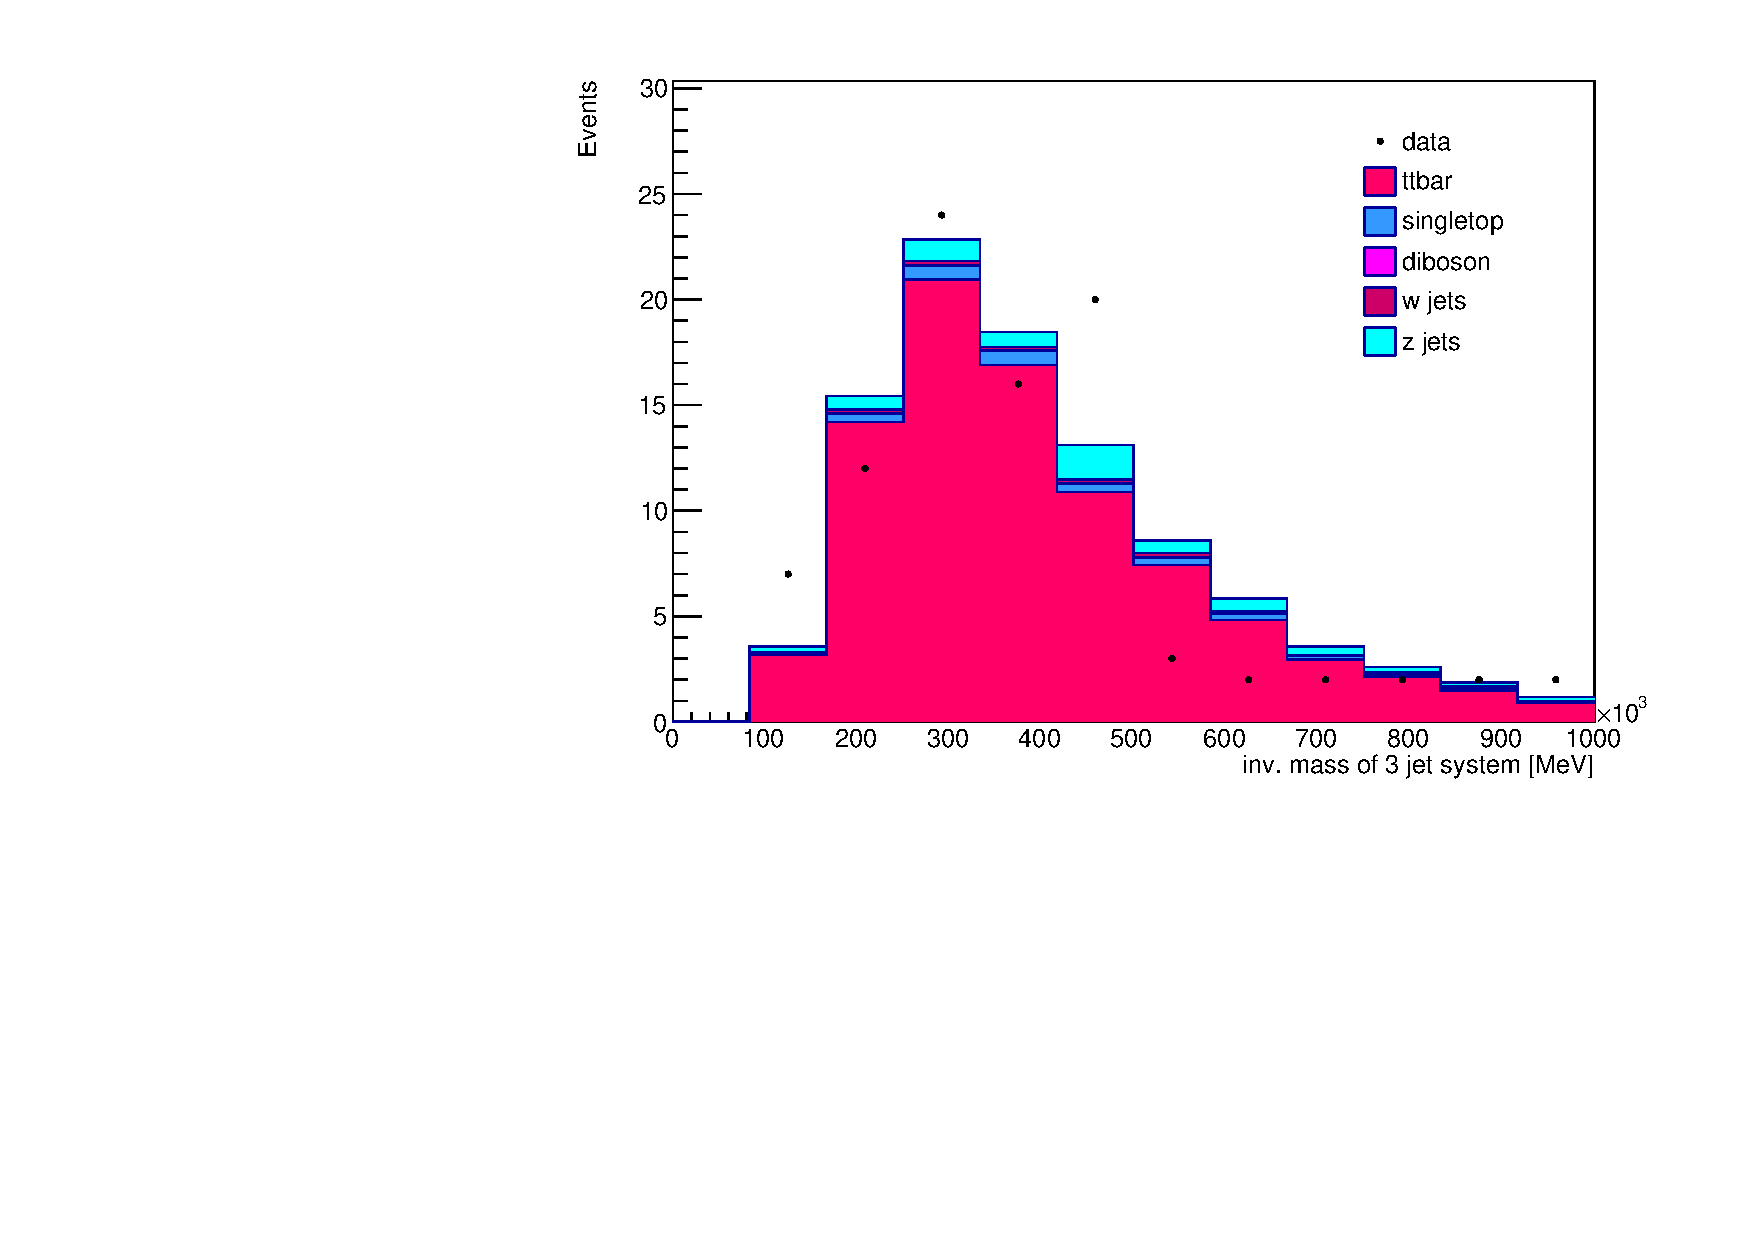
\includegraphics[width=\linewidth]{plots_and_txt/stacked_plots/stacked_3JetSys.pdf}
    \caption{}
    \label{fig:stacked_3jetsys}
  \end{subfigure}%
  \begin{subfigure}{0.5\textwidth}
    \centering
    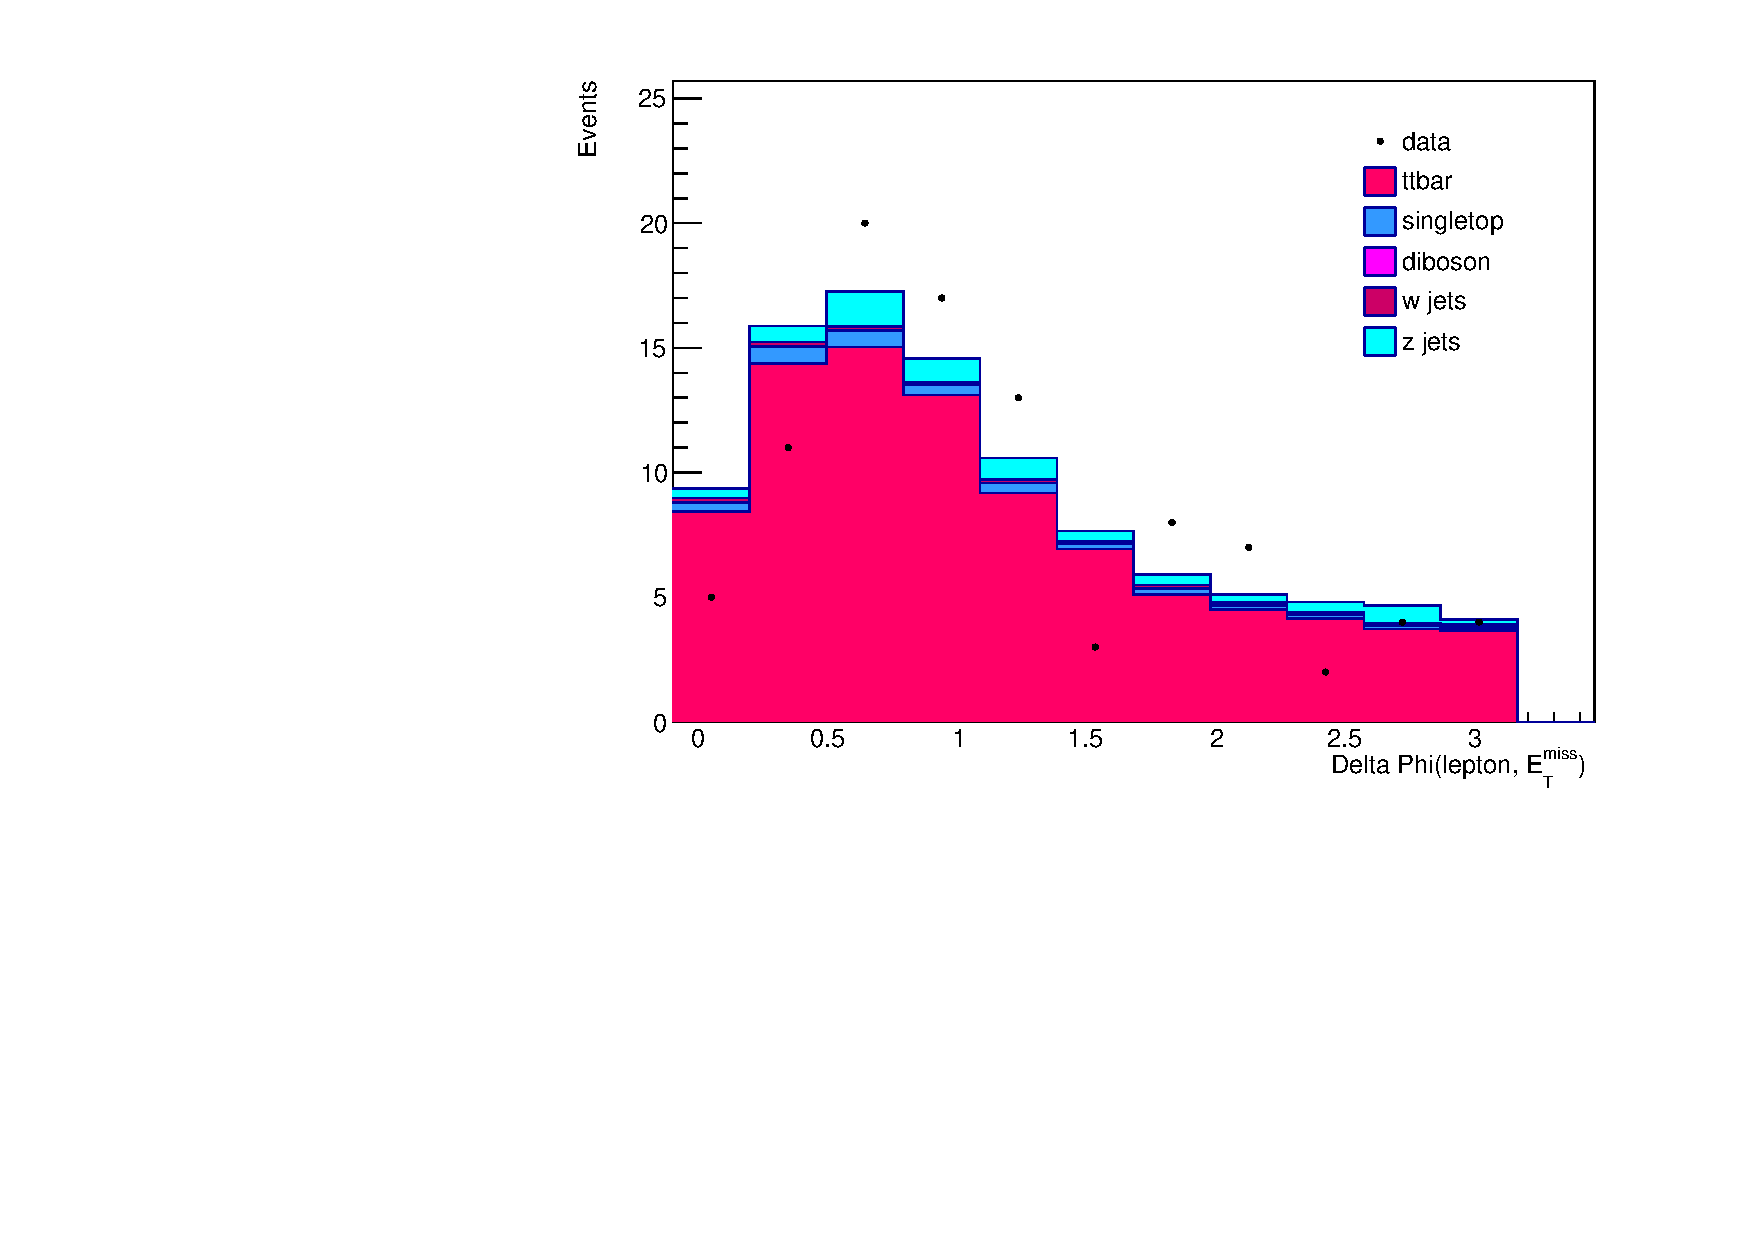
\includegraphics[width=\linewidth]{plots_and_txt/stacked_plots/stacked_deltaphi.pdf}
    \caption{}
    \label{fig:stacked_deltaphi}
  \end{subfigure}%
  \newline
  \begin{subfigure}{0.5\textwidth}
    \centering
    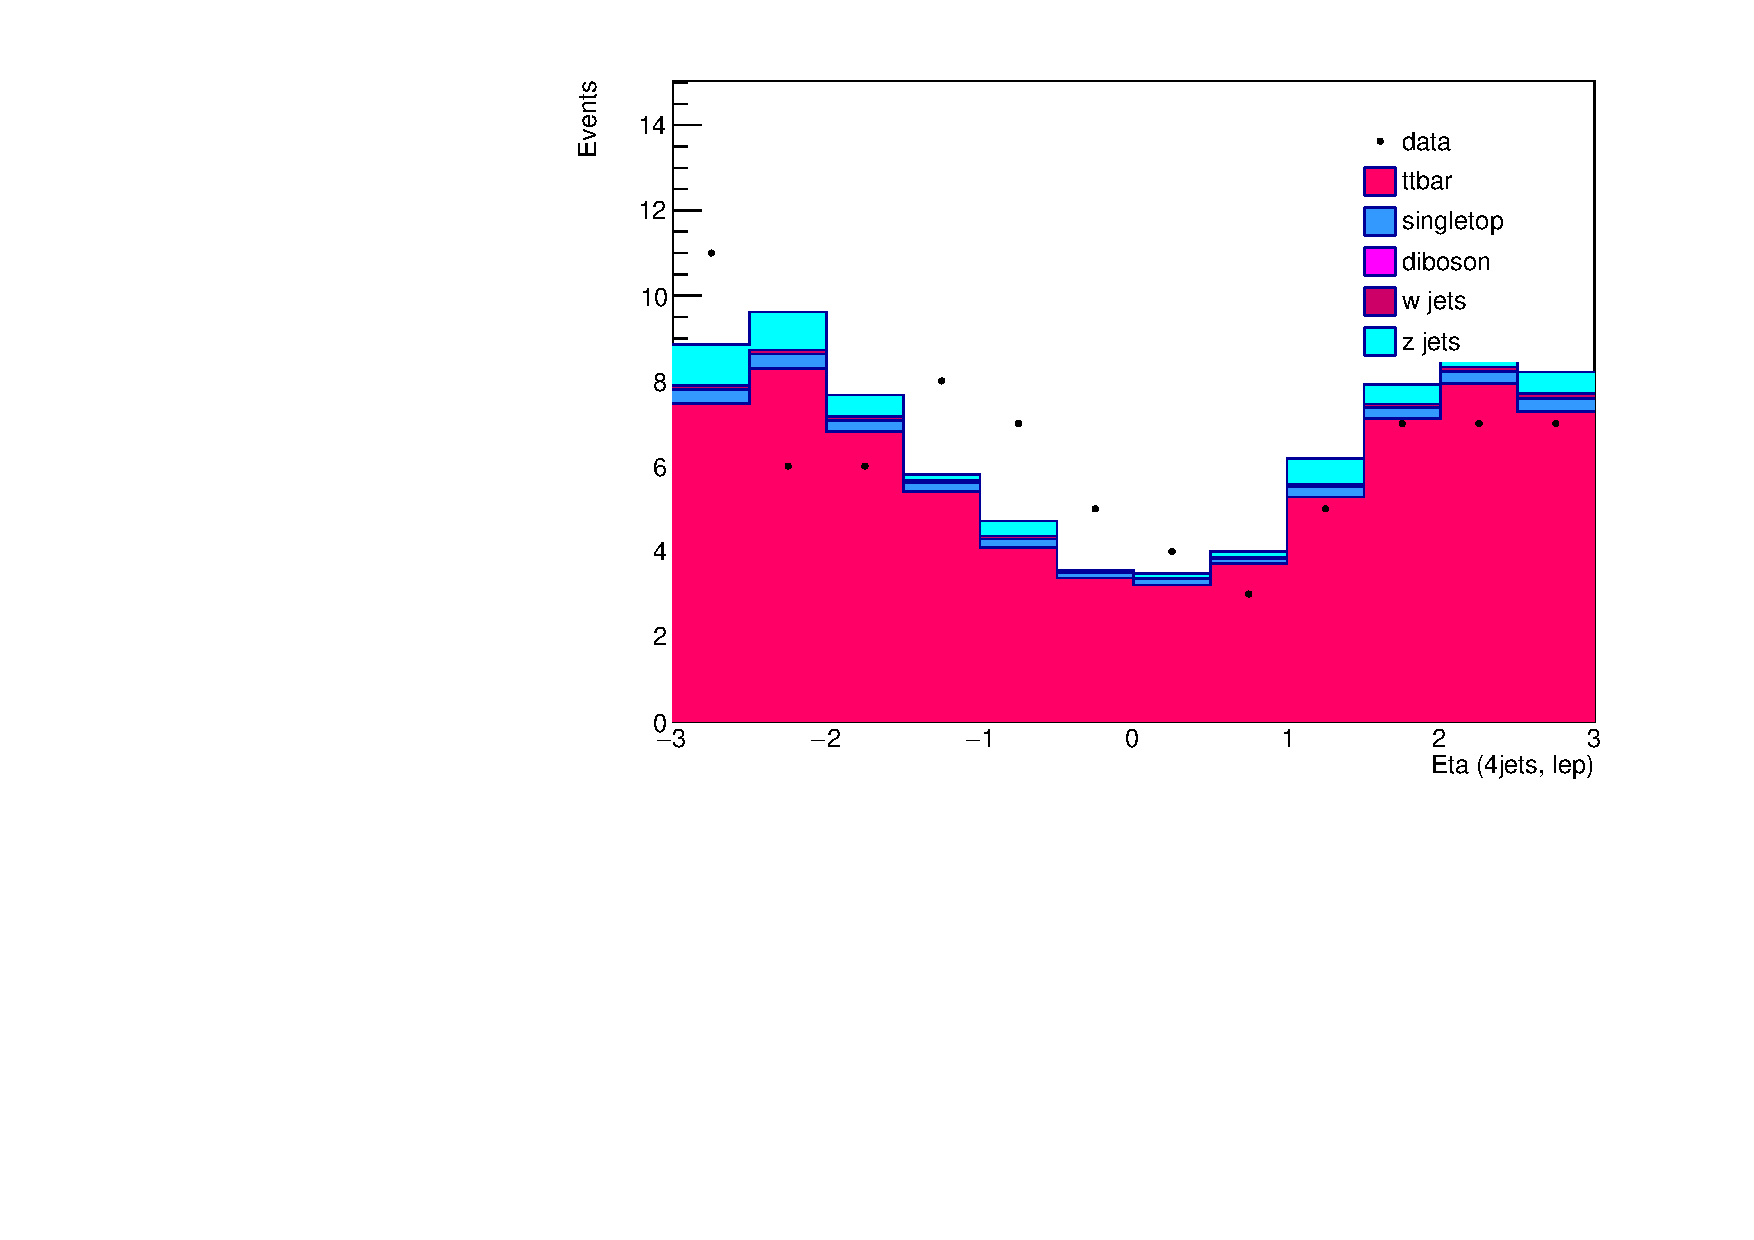
\includegraphics[width=\linewidth]{plots_and_txt/stacked_plots/stacked_fulleta.pdf}
    \caption{}
    \label{fig:stacked_fulleta}
  \end{subfigure}%
  \caption{Darstellung verschiedener Stacked Plots als Überprüfung der Übereinstimmung von Simulation und Daten.
  Zusehen ist die invariante des Dreijetsystems aus den drei Jets mit dem höchsten $p_T$ (\subref{fig:stacked_3jetsys}),  
  der Azimuthwinkel zwischen der fehlenden Transversalenergie und dem geladenen 
  Lepton (\subref{fig:stacked_deltaphi}) und die Pseudorapidität des gesamten Systems (geformt aus den vier Jets mit dem größten $p_T$, dem Lepton und dem 
  Neutrino) (\subref{fig:stacked_fulleta}).
  }
  \label{fig:stacked_Distributions4}
\end{figure}












%_
